\documentclass[]{TimStyle}
%\documentclass[]{uzhpubTim}
%\documentclass[]{scrreprt}


% customize dictum format:
\setkomafont{dictumtext}{\itshape\small}
\setkomafont{dictumauthor}{\normalfont}
\renewcommand*\dictumwidth{\linewidth}
\renewcommand*\dictumauthorformat[1]{--- #1}
\renewcommand*\dictumrule{}

%input
\usepackage[latin1]{inputenc}

\usepackage[autostyle, english = american]{csquotes}

\usepackage[official]{eurosym}%for Euro symbol

%bibliography
\usepackage[backend=biber, doi=false , isbn=false, authordate, noibid,bibencoding=utf8, giveninits=true]{biblatex-chicago}
\urlstyle{sf} % better deals with url breaks
\AtEveryBibitem{\clearfield{month}} % cleaner formatting of volume (issue)

%\addbibresource{BiblioNeutralSimul.bib}
%\addbibresource{BiblioDecPopDyn.bib}
\addbibresource{BiblioTotal.bib}

%Layout
\usepackage[T1]{fontenc}
\usepackage{geometry}
\usepackage{tocloft}
\usepackage{footmisc}
\usepackage{enumitem}

\usepackage{setspace}   %Allows double spacing with the \doublespacing command

\usepackage[normalem]{ulem}%underlining _ normalem option necessary not to interact with biblatex
%\usepackage[round]{natbib}%

%Figures
\usepackage{graphicx}%
\usepackage{float}%
\floatplacement{figure}{ht}

%Tables
\usepackage{multirow}%
\usepackage{booktabs}%
%Maths
\usepackage{mathtools}%
\usepackage{amsmath}%
\usepackage{amsthm}%
\usepackage{amsfonts}%

%Miscellaneous
\usepackage{pifont}%for funny symbols

%Home made commands
\usepackage{xspace}% to avoid annoyance with spaces when using macros
\newcommand{\NSM}{NS\xspace}
\newcommand{\MM}{MM\xspace}
\newcommand{\Cov}{\mathrm{cov}}

\newcommand{\sh}{$s_0h_-$\xspace}
\newcommand{\sH}{$s_0h_+$\xspace}
\newcommand{\Sh}{$s_+h_-$\xspace}
\newcommand{\SH}{$s_+h_+$\xspace}
\newcommand{\Range}[3]{$#1 \; [#2 ; #3 ]$}

\usepackage{hyperref} % Required for adding links	and customizing them
% Always must be last package!!
%%%%%%%%%%%%%%%%%%%

\title{Individual-level causes and population-level\\consequences of variation in fitness in an alpine rodent}
%\subtitle{PhD dissertation}
\author{Timoth\'{e}e Bonnet}

\date{August 2016}

\begin{document}
%\maketitle
\begin{titlepage}
	\thispagestyle{empty}
    \begin{center}
        %{\fontsize{22}{36	pt}\selectfont\upshape\bfseries\textbf{Individual-level causes and population-level consequences of variation in fitness in an alpine rodent}}
				 {\onehalfspacing \LARGE\selectfont\upshape\bfseries{Individual-level causes and population-level\\consequences of variation in fitness in an\\alpine rodent\\}}
				
				\vspace{1cm}
				
				\noindent\makebox[\linewidth]{\rule{0.8\paperwidth}{1pt}}
        
        \vspace{1cm}
				{\fontsize{22}{32pt}
				\doublespacing
        Dissertation
				\\
				zur
				\\
				Erlangung der naturwissenschaftlichen Doktorw\"urde
				\\
        (Dr. sc. nat.)
				\\
				Mathematisch-naturwissenschaftlichen Fakult\"at
				\\
				der
				\\
				Universit\"at Z\"urich
				\\
				von
				\\
        \vspace{1cm}
        \textbf{Timoth\'ee Bonnet}
        \\
				aus
				\\
				Frankreich
				
				\vspace{1cm}
				\textbf{Promotionskomitee}
				\\
				Prof. Dr. Lukas Keller (Vorsitz)
				\\
				Dr. Erik Postma (Leitung der Dissertation)
				\\
				Prof. Dr. Barbara Tschirren
				\\
				Prof. Dr. Arpat Ozgul
				\\
				Dr. Jarrod Hadfield
				\\
				Dr. Marc K\'ery
				\\
				}
        \vfill
        
        \textbf{Z\"urich, 2016}
    \end{center}
	
\end{titlepage}

	\clearpage
\begin{titlepage}
	\thispagestyle{empty}

\null\vfill
\noindent \copyright  Timoth\'ee Bonnet\\
\href{mailto:timotheebonnetc@gmail.com}{timotheebonnetc@gmail.com}\\
Photos: Timoth\'ee Bonnet\\
This is a \LaTeX document using a customized version of the KOMA-Script's class \texttt{scrbook}
\end{titlepage}

\frontmatter
\addcontentsline{toc}{chapter}{Summary}
\begin{summary}
\textbf{
This thesis investigates the stochastic and selective causes of variation in fitness components, and the evolutionary consequences of this variation in a wild rodent population. 
It shows the contemporary genetic evolution of body mass and decouples classic estimates of selection from adaptive evolution. 
}

The heart of evolutionary biology is understanding the variation in organisms. For over 150 years, researchers have documented the causes of within-species variation and how it contributes to speciation and explains the fit between organisms and their environment. 
Recently, increasing concerns regarding rapid anthropogenic changes have driven renewed investigation of how wild populations adapt to environmental change.
This new focus has revealed the difficulties measuring natural selection, disentangling evolution from plastic changes, and predicting evolutionary trajectories. 
For instance, there are few robust examples of contemporary evolution in wild populations, casting doubt on the possibility that evolution can rescue populations from rapid environmental change.
In this thesis, I investigate the causes of natural selection and evolution in a wild population of snow voles (\textit{Chionomys nivalis}). Thanks to 10 years of intensive individual-based monitoring and genotyping, knowledge of this population includes life-history, morphological data, and a high-resolution pedigree. This population is therefore among the best available worldwide to measure selection and evolution in action. 

The population is nevertheless relatively small and recent publications suggest that the evolutionary potential in small populations is effectively cancelled by stochasticity in fitness components. I assess the methods used in those publications and demonstrate that the variation in fitness components is not purely stochastic. Small populations, including these snow voles, show evolutionary potential. 
 
With collaborators, I then compare four common methodological frameworks to disentangle the contributions to phenotypic change of evolution, plasticity, and demography. We identify important discrepancies between the frameworks, partly originating from using different definitions, but also possessing intrinsically different capabilities. Among the considered frameworks only quantitative genetics can measure genetic change.

Applying methods from quantitative genetics to the snow vole population, I demonstrate that body mass evolved adaptively over the study period. I show that phenotypic estimates of selection are not predictive of genetic evolution: neither the mean selection nor its temporal variation are related to the rate of genetic evolution. This demonstrates that the dominant purely-phenotypic method used to measure selection risks measuring variation in nutritional status instead. Nevertheless, I employed quantitative genetics to identify the target of selection and obtain selection estimates in line with the observed genetic change 

This thesis establishes contemporary evolution in a wild population and shows that evolutionary responses to environmental change cannot be reliably estimated nor understood from purely-phenotypic methods; an explicit genetic approach is necessary. 

\end{summary}


\addcontentsline{toc}{chapter}{Zusammenfassung}
\begin{zusammenfassung}
\addcontentsline{toc}{chapter}{Zusammenfassung}
\textbf{Diese Doktorarbeit untersucht die stochastischen und selektiven Ursachen der Variation in Fitnesskomponenten und deren evolution{\"a}ren Konsequenzen in einer freilebenden Nagetierpopulation. Sie zeigt die gegenw{\"a}rtige, genetische Evolution von K{\"o}rpermasse und entkoppelt klassische Selektionssch{\"a}tzungen von adaptiver Evolution.}

Das Herzst{\"u}ck der Evolutionsbiologie liegt im Verst{\"a}ndnis der Vielfalt von Organismen. W{\"a}hrend {\"u}ber 150 Jahren haben Forscher die Ursachen von intraspezifischer Variation dokumentiert, wie sie zur Artbildung beitr{\"a}gt und zum Zusammenpassen von Organismen mit ihrer Umwelt. Zunehmende Bedenken wegen der schnellen anthropogenischen Ver{\"a}nderungen haben in letzter Zeit eine erneute Erforschung, wie sich freilebende Populationen an Umweltver{\"a}nderungen anpassen, vorangetrieben. Dieser neue Fokus offenbart die Schwierigkeiten im Messen von nat{\"u}rlicher Selektion, die Entflechtung von Evolution und plastischen Ver{\"a}nderungen und dem Vorhersagen von evolution{\"a}ren Entwicklungsverl{\"a}ufen. Unter anderem gibt es nur wenige robuste Beispiele von gegenw{\"a}rtiger Evolution in freilebenden Populationen, die, die M{\"o}glichkeit, dass Evolution Populationen bei schnellen Ver{\"a}nderungen der Umweltbedingungen rettet, fraglich erscheinen l{\"a}sst. In dieser Doktorarbeit erforsche ich die Ursachen nat{\"u}rlicher Selektion und Evolution in einer freilebenden Population von Schneem{\"a}usen (\textit{Chionomys nivalis}). Dank 10 Jahren intensivem Individuen-basiertem Monitoring und Genotypisierung, beinhaltet der Erkenntnisstand dieser Population Lebensweise, morphologische Daten und einen hochaufgel{\"o}sten Stammbaum. Deswegen ist diese Population unter den besten weltweit verf{\"u}gbaren um Selektion und Evolution in Aktion zu messen. 

Trotzdem ist die Population ziemlich klein und neuerliche Publikationen legen nahe, dass das evolution{\"a}re Potential in kleinen Populationen effektiv von Stochastik in Fitnesskomponenten aufgehoben wird. Ich beurteile diese Methoden, die in diesen Publikationen benutzt wurden und demonstriere, dass die Variation in Fitnesskomponenten nicht ausschliesslich stochastisch ist. Kleine Populationen, einschliesslich diese Schneem{\"a}use, zeigen evolution{\"a}res Potential. 

Mit Kollaboratoren vergleiche ich dann vier h{\"a}ufig benutzte methodologische Ans{\"a}tze um die Anteile von Evolution, Plastizit{\"a}t und Demographie an der ph{\"a}notypischen Ver{\"a}nderung zu entflechten. Wir identifizieren wichtige Unstimmigkeiten zwischen den Ans{\"a}tzen, die teilweise vom Gebrauch von unterschiedlichen Definitionen, aber auch vom Besitz von intrinsisch unterschiedlichen F{\"a}higkeiten stammen. Unter den in Betracht gezogenen Ans{\"a}tzen kann nur quantitative Genetik genetische Ver{\"a}nderungen messen. 

Durch die Anwendung von quantitativ-genetischen Methoden an der Schneemaus-Population demonstriere ich, dass sich K{\"o}rpermasse {\"u}ber die Studiendauer adaptiv entwickelt. Ich zeige auf, dass ph{\"a}notypische Sch{\"a}tzungen von Selektion nicht genetische Evolution hervorsagen: weder die durchschnittliche Selektion noch die temporale Variation h{\"a}ngen mit der Rate genetischer Evolution zusammen. Das legt dar, dass die dominante, rein ph{\"a}notypische Methode zur Messung von Selektion stattdessen die Messung von Variation im Ern{\"a}hrungszustand riskiert. Dennoch habe ich quantitative Genetik zur Identifikation von Selektion verwendet und Selektionssch{\"a}tzungen erhalten, die  mit der beobachteten genetischen Ver{\"a}nderung {\"u}bereinstimmen. 

Diese Doktorarbeit weist gegenw{\"a}rtige Evolution in einer freilebenden Population nach und zeigt dass evolution{\"a}re Reaktionen auf Umweltver{\"a}nderungen  von rein ph{\"a}notypischen Methoden weder zuverl{\"a}ssig eingesch{\"a}tzt noch verstanden werden k{\"o}nnen; ein expliziter, genetischer Ansatz ist notwendig. 
\end{zusammenfassung}


\setcounter{tocdepth}{0}
\tableofcontents 

%%%%%%%%%%%%%%%%%%%%%%%%%%%%%%%%%% Start Chapters
\mainmatter


\begin{refsection}
\setchapterpreamble[ur][.6\textwidth]{%
\dictum[Fyodor Dostoyevsky, \textit{The Idiot} (1868--9)]{%
One can't understand everything at once, we can't begin with perfection all at once! In order to reach perfection one must begin by being ignorant of a great deal. And if we understand things too quickly, perhaps we shan't understand them thoroughly.}\vskip1em

\dictum[dude]{%
things}\vskip1em}

\chapter[Chapter 1: General introduction]{General introduction}
\chaptermark{General introduction}
%%%%%%%%%%%%%%%%%%%%%%%%%%%%%%%%%%%%%%%%%%%%%%%%%%%%%%%%%%%%%%%%%%%%%%%%%%%%%%%%%%%%%%

%%%%%%%%%%%%%%%%%%%%%%%%%%%%%%%%%%%%%%%%%%%
\section{Variation in fitness}
%variation in evolution
Understanding variation among living things is the heart of evolutionary questioning.


Darwin great discovery was to recognize the variation within species as the fuel generating the astonishing diversity of species themselves.

%fitness
There has been a great deal written about the concept of fitness, and as is common for central scientific concepts REF?, its definition is problematic. Actually, there are many definitions, and sub-definitions. 
In this thesis, what we mean by \emph{fitness} is ...
most adapted to the study framework.
with the difficulty that... 


In this thesis, we will not really deal with the fundamental question of appearance and maintenance of variation in fitness (e.g. lek paradox, see XX), but rather with its proximal sources.

 
%%%%%%%%%%%%%%%%%%%%%%%%%%%%%%%%%%%%%%%%%%%
\section{Quantitative genetics}

How to measure and make sense of genetic variation?
For over a century, there have been two main approaches. 
These can be summarized as ``bottom-up'' and ``top-down''.
The Mendelians and the biometricians



intronic region of the fat metabolism and food intake-related \emph{lepr} gene

We found a recessive allele (let call the recessive allele \emph{a}, and the dominant allele \emph{A}) associated with lighter individuals (Fig. \ref{fig:leprpheno}). Homozygotes \emph{aa} were -2.9 g lighter (95\% credibility interval $[0.6;5.1]$), that is, 8\% lighter than the mean. 


\begin{figure}[ht]
	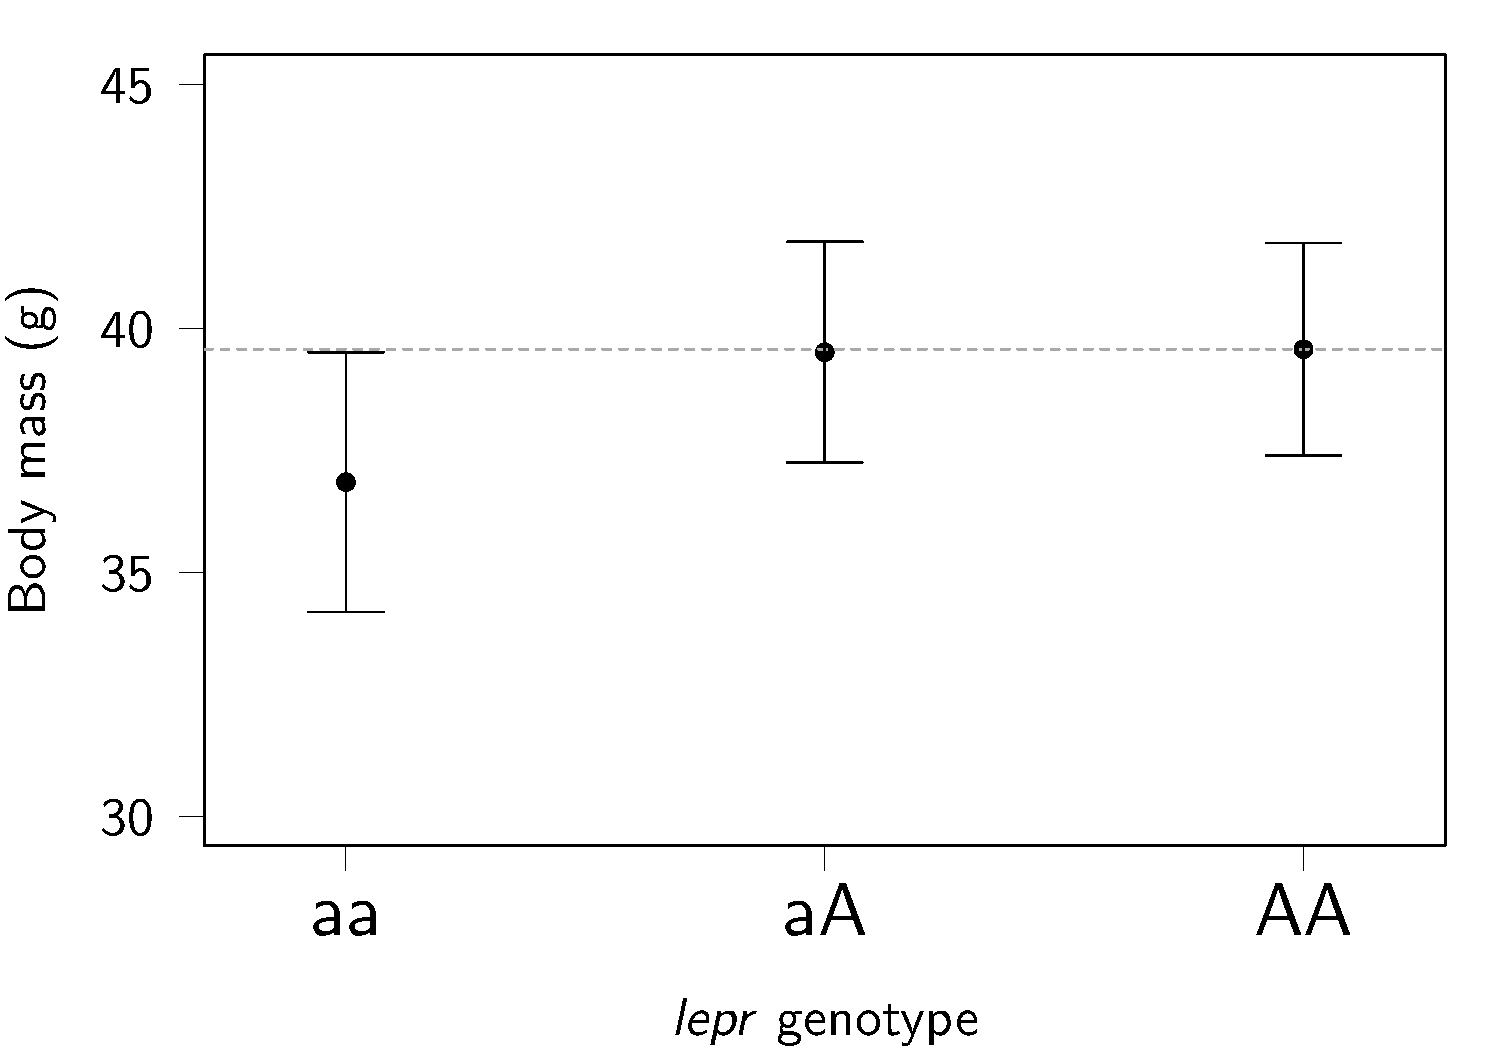
\includegraphics[width=1\textwidth]{FiguresGeneral/PhenoEffect-1}
	\caption{Expected body mass of snow voles bearing the three \emph{lepr} genotypes. The expectations and 95\% confidence intervals were predicted from a linear mixed model fitted to the 2311 mass measurement of 532 snow voles. The model accounted for sex, age, date of capture and their two-ways interactions, as well as year of capture and multiple measurements of the same individual.}
	\label{fig:leprpheno}
\end{figure}

Despite such a dramatic effect, \emph{lepr} genotypic variation explains only 1.3\% of the additive genetic variation estimated from an animal model. This proportion can seem small, but in particular because the homozygotes \emph{aa} are rare (3\% of all individuals genotyped).

Could we not simply sequence many more genes to explain a larger proportion of genetic variation?
The uncertainty in the estimation of the effect of \emph{lepr} translates into a Bayesian p-value of $0.01$. 
If other genetic loci were analysed, 


%%%%%%%%%%%%%%%%%%%%%%%%%%%%%%%%%%%%%%%%%%%
\section{This thesis}

\subsection{Objectives}

\subsection{Churwalden snow voles}

\subsection{Thesis outline}



\end{refsection}

\begin{refsection}
\setchapterpreamble[ur][.6\textwidth]{%
\dictum[Eiji Yoshikawa, \textit{Musashi} (1935)]{%
If the talents I was born with are the right ones, I may someday achieve my goal. If not, I may go through life being as stupid as I am now.}\vskip1em
\dictum[Jean-Paul Sartre, \textit{La naus\'ee} (1938)]{%
Quand on veut comprendre une chose, on se place en face d'elle, tout seul, sans secours; tout le pass\'e du monde ne pourrait servir de rien. Et puis elle dispara\^{i}t et ce qu'on a compris dispara\^{i}t avec elle.}\vskip1em
}

\chapter[Successful by chance?]{Successful by chance? The power of mixed models and neutral simulations for the detection of individual fixed heterogeneity in fitness components}

\textbf{Timoth\'{e}e Bonnet*} and Erik Postma (2016) The American Naturalist 187(1):60-74\\

\section{Abstract}
Heterogeneity in fitness components consists of fixed heterogeneity due to latent differences fixed throughout life (e.g. genetic variation), and dynamic heterogeneity generated by stochastic variation. Their relative magnitude is crucial for evolutionary processes, as only the former may allow for adaptation. 
However, the importance of fixed heterogeneity in small populations has recently been questioned. Using neutral simulations (\NSM), several studies failed to detect fixed heterogeneity, thus challenging previous results from mixed models (\MM).
To understand the causes of this discrepancy, we estimate the statistical power and false positive rate of both methods, and apply them to empirical data from a wild rodent population.
    While \MM show high false positive rates if confounding factors are not accounted for, they have high statistical power to detect real fixed heterogeneity. In contrast, \NSM are also subject to high false positive rates, but always have low power. Indeed, \MM analyses of the rodent population data show significant fixed heterogeneity in reproductive success, whereas \NSM analyses do not.
   We suggest that fixed heterogeneity may be more common than is suggested by \NSM, and that \NSM are useful only if more powerful methods are not applicable and if they are complemented by a power analysis.

\textbf{Keywords: } \textit{Chionomys nivalis}; individual-based model; generalized linear mixed model; simulations; snow vole; statistical power\\
\textbf{Online enhancements: }
Online appendices. Data available from the Dryad Digital Repository: \url{http://dx.doi.org/10.5061/dryad.3cb61}.

\section{Introduction}

Within species, individual variation in lifetime reproductive success (LRS) is plentiful, with most individuals producing few or no offspring and a few individuals producing a large share of the next generation \parencite{Clutton1988,Stearns1992}. Given their skewed and heterogeneous nature, LRS distributions are unlikely to be solely shaped by unstructured environmental stochasticity. Instead, individuals seem to differ in their probability of surviving or reproducing \parencite{Kendall2011}.

Often, this individual heterogeneity in LRS is assumed to originate from latent individual differences which are fixed throughout an individual's life, i.e. that there is individual heterogeneity in frailty, quality or fitness \parencite[e.g.][]{Vaupel1979,Morris1998, Cam2000}. This is commonly referred to as fixed heterogeneity. Genetic variation is one source of fixed heterogeneity \parencite[e.g.][]{Keller2002,Ellegren2008}, but epigenetic, maternal and permanent environmental effects may also be important \parencite{Wolf2009,Turner2009}. This fixed variation is usually measured retrospectively; in some cases it may have arisen at fertilization, but it may also be shaped by the environment an individual experiences throughout its life, for instance through variation in habitat choice or through gene by environment interactions. It is important to distinguish fixed heterogeneity as it is used here\textemdash that is, the repeatability of individual performance\textemdash from other sources of variation that are not due to the properties of individuals (e.g. climatic variations among years). Indeed, only fixed differences among individuals can be the target of selection and allow for adaptation, provided that these fixed differences are passed on to the next generation\textemdash be it through genes \parencite{Keller2002}, philopatry \parencite{Schauber2011} or other processes \parencite{Bonduriansky2012}. 

Recent publications \parencite{Tuljapurkar2009,Steiner2010,Orzack2011,Steiner2012} have argued forcefully that invoking fixed differences among individuals (i.e. fixed heterogeneity) in fitness components is rarely required to explain the observed heterogeneity in LRS. Instead, they emphasize that due to the stochasticity of individual life histories, individual heterogeneity is expected even in populations of identical individuals \parencite{Caswell2011}. Indeed, if individuals take a random trajectory through the various life-history stages, and if these stages are associated with differential reproductive and survival rates, the population-level distribution of LRS may be skewed and heterogeneous. This type of heterogeneity is referred to as dynamic heterogeneity \parencite{Tuljapurkar2009}. Crucially, dynamic heterogeneity originates from differences among life stages, whereas fixed heterogeneity originates from variation in the properties of individuals.

Given that most life-history traits are heritable to some degree \parencite{Mousseau1987, Postma2014}, it is beyond doubt that some fixed heterogeneity is present in most wild populations. At the same time, the cumulative effects of individual histories on their realized lifespan and reproductive success are also unquestionable \parencite{Caswell2011}. What is subject to discussion, however, is the relative importance of fixed, versus dynamic, heterogeneity in shaping variation in LRS. \cite{Steiner2012} suggested that, at least in small populations, the drift generated by large life-history stochasticity is too large for fixed heterogeneity to play a significant role in shaping evolution and demography at the level of a single population. Instead, they have proposed dynamic heterogeneity as the null model to explain any observed heterogeneity. Only if this null model can be rejected should we consider an additional role for fixed heterogeneity in shaping variation in LRS or fitness components. 

\cite{Tuljapurkar2009} have suggested that an appropriate tool to test for fixed heterogeneity is provided by neutral simulations (\NSM hereafter), which generate summary statistics describing the distribution of LRS and the pattern of life-stage transitions expected in the absence of fixed heterogeneity. These expectations can subsequently be compared to their observed counterparts to detect departures from neutrality due to the existence of fixed heterogeneity. 

The application of \NSM to data for two sea bird populations \parencite{Steiner2010,Orzack2011}, as well as to a compilation of 22 vertebrate populations \parencite{Tuljapurkar2009} has been unable to reject the null hypothesis of neutrality, leading to the conclusion that dynamic heterogeneity alone can explain the observed variation in life histories in most populations. Indeed, we are aware of only one study in which \NSM rejected neutrality, for one of three reproductive parameters in a roe deer population \parencite{Plard2012}. 

In contrast to studies relying on \NSM, studies employing linear mixed models (hereafter \MM) commonly report evidence for fixed heterogeneity \parencite[e.g.][] {Cam2000,Royle2008,Chambert2013,Guillemain2013,Chambert2014}. Interestingly, \cite{Cam2013} have provided evidence for fixed heterogeneity in a data set for which the existence of fixed heterogeneity had been dismissed based on \NSM \parencite{Steiner2010}. However, \MM and \NSM differ in how they deal with data: \MM rely on repeated measurements of individuals, while \NSM use summary statistics aggregated at the population level. Compared to \MM, \NSM are thus less data-demanding, but might be less sensitive to statistical signals at the individual level. On the other hand, aggregation might allow \NSM to detect effects that emerge only at the population level and are invisible to \MM.
More formally, the discrepancy between \NSM and \MM suggests that they differ in either their type I (i.e. false positive) error rate, or in their type II error rate (i.e. power). For instance, the opposite conclusions reached by \NSM in \cite{Steiner2010} and \MM in \cite{Cam2013} may be the result of the statistical power of the \NSM being too low, preventing the detection of fixed heterogeneity (i.e. a type II error). Alternatively, \MM may have high rates of type I error, if the individual-level variances estimated by the \MM are spurious, or they are unduly interpreted as the mark of fixed heterogeneity.

Applying both methods to data with known properties allows for the estimation of both types of error rates and thereby provides insight into the ability of both methods to detect fixed heterogeneity. Unfortunately however, fixed heterogeneity is the result of latent, unobservable traits, which cannot be inferred without a modeling step \parencite{Cam2013}, and it is precisely the performance of this modeling step that we investigate here. Computer simulations provide a way around this problem, as they allow one to apply methods to data sets with known underlying properties \parencite[e.g.][]{DeVillemereuil2013,Brooks2013}.

Here, we simulate a series of longitudinal, individual-based, data sets through an algorithm that introduces varying amounts of fixed and dynamic heterogeneity in survival and reproduction. For illustrative purposes, these simulations are parametrized to match a population of snow voles (\textit{Chionomys nivalis}, Martins 1842) located in the Swiss Alps. In order to assess the type I and type II error rates of both \NSM and \MM, we subsequently analyze the simulated data sets using both methods. In a final step, we use these results to interpret the results of the application of both methods to the real snow vole data set. Figure \ref{figure:flow} shows a diagram summarizing our approach. Altogether, our results highlight the lack of statistical power of \NSM, but at the same time emphasize that \MM output should be interpreted with care. We discuss the origin of the discrepancy between \NSM and \MM, and what this tells us about the nature of biological variability.

\section{Material and methods}

\subsection{Data simulation}

The simulation model matches the life cycle of the population of snow voles which we use in the empirical comparison of both methods. The monitoring of this population is discussed in some detail in Appendix \ref{ap:snv}. Only two age classes are modeled (non-reproducing juveniles and reproducing adults), and there are no sex-specific or spatio-temporal effects on fitness components, as the uncertainty with respect to the appropriate specification of these models would introduce an additional layer of complexity \parencite[see e.g.][]{Cam2013}.
All simulated populations are monitored for 10 years. For every individual, we have perfect knowledge of survival and reproduction during the study period, but their fate beyond this period is unknown. Every year, a new cohort of 100 juveniles appears. After one year, these juveniles become adults and start reproducing. Every year, adults can reproduce once; the number of offspring produced by an individual is labeled annual reproductive success (ARS). In the real snow vole population, there is no apparent senescence in survival and the maximum age observed is four years old. Accordingly, in the simulations, adult survival probability does not vary with age until the fourth year, but all individuals still alive at that point die during the next winter. Mortality events occur after birth for juveniles and after reproduction for adults. A single sex is simulated, as the two sexes are generally analyzed separately in \NSM, and in \MM sex differences in the mean are accounted for by fitting sex as a fixed factor.

We define a scenario as a collection of simulation parameters. For each scenario, 1000 data sets were simulated, that is 1000 putative populations with the same underlying properties. In an attempt to detect evidence for fixed heterogeneity, each data set was then analyzed using \MM and \NSM. Note the potential for confusion between the simulation of the data sets on the one hand, and the neutral simulation method on the other. The latter is always referred to as \NSM. Simulations were carried out using a C++ program (available at \verb+https://github.com/timotheenivalis/FixDynHet+), using the pseudo-random number generator \verb+Mersenne Twister+ \parencite{Matsumoto1998} and a command file procedure following that of \verb+IBDsim+ \parencite{Leblois2009}. The analyses of the simulation output were all conducted in \verb+R 3.1.0+ \parencite{R2014}, using the package \verb+lme4+ (version 1.1-7) \parencite{Bates2014a}.

Due to demographic stochasticity \parencite[sensu][]{Fox2002}, all simulated data sets contain a baseline level of dynamic heterogeneity. Indeed, according to \cite{Tuljapurkar2009}, the presence of dynamic heterogeneity results in the ``scaled sequence entropy of the transition matrix between reproductive stages'' (hereafter simply referred to as entropy), being greater than zero, which is always the case here. Entropy measures the rate at which the diversity of life-history trajectories increases with their length, which is due to random transitions between stages with different survival probabilities and reproductive outcomes \parencite{Tuljapurkar2009}.

Beyond this baseline level of dynamic heterogeneity, heterogeneity in fitness components is introduced either as explicit fixed heterogeneity, or through a Markovian process. For the simulation of fixed heterogeneity, at birth, each individual receives a fixed quality as reproducer and survivor. These fixed qualities do not change over the course of its life. Therefore, some individuals intrinsically have a high probability to perform well, and some individuals have a high probability to perform poorly, irrespective of their past performance, as in a classic frailty model \parencite{Vaupel1979}. In contrast, for the simulations using a Markovian process, an individual's probability to survive and to achieve a certain ARS is not fixed, but changes at each time step and depends solely on its ARS the time step before. Therefore, these data contain dynamic heterogeneity only. However, some of this mimics fixed heterogeneity because individual performances can persist over time. Generalized linear mixed models were used to check that the properties of the simulated data sets matched the model and the parameters used to generate them (see Appendix \ref{ap:chpro}).

\paragraph{Simulations with explicit fixed heterogeneity}
At birth, every individual receives a quality as reproducer $q_{\rho,i}$, which is normally distributed with a mean of 0 and a variance equal to $\sigma_{\rho}^2$, i.e. \mbox{$q_{\rho,i}\sim$ {\fontfamily{pzc}\selectfont N }$(0,\sigma_{\rho}^2)$.} Individuals also receive a quality as survivor $q_{\phi,i}$, with \mbox{$q_{\phi,i}\sim$ {\fontfamily{pzc}\selectfont N }$(0,\sigma_{\phi}^2)$.} These qualities are fixed for the lifetime of an individual. Because trade-offs between survival and reproduction are not considered here, the two qualities are drawn independently for each individual. The variances $\sigma_{\rho}^2$ and $\sigma_{\phi}^2$ represent the amount of fixed heterogeneity in reproduction and survival, respectively. 

If individual $i$ is an adult at time $t$, its annual reproductive success, $\rho_{i,t}$, is drawn from a Poisson distribution,

\begin{equation}
\rho_{i,t} \sim \text{{\fontfamily{pzc}\selectfont P }}(\exp(\log(\mu_{\rho})+q_{\rho,i}))\text{,}
\end{equation}
where $\mu_{\rho}$ is the mean annual reproductive success. For an individual with $q_{\rho,i}=0$, i.e. the average individual in a population with fixed heterogeneity, the parameter of the Poisson distribution ($\exp(\mathrm{log}(\mu_{\rho})+q_{\rho,i})$) reduces to the population mean ARS ($\mu_{\rho}$). The qualities for reproduction ($q_{\rho,.}$) are normally distributed on the log-transformed scale of ARS.

The survival outcome of an individual $i$ at time $t$, $\phi_{i,t}$, is zero (death) if the individual is four years old, and otherwise is drawn from a Bernoulli distribution:

\begin{equation}
\phi_{i,t} \sim \text{{\fontfamily{pzc}\selectfont B }}( \mathrm{logit}^{-1}(\mathrm{logit}(\mu_{\phi}+j_{i,t}\beta_{j})+q_{\phi,i})) \text{,}
\end{equation} 
where $\mathrm{logit}(p)= \mathrm{log}(\frac{p}{1-p})$ and its inverse function $\mathrm{logit}^{-1}(x)=\frac{1}{1+\exp(-x)}$, where $j_{i,t}$ is a Boolean variable equal to 0 for adults and 1 for juveniles, and where $\beta_{j}$ is the difference between the mean survival probability of juveniles and adults. For an individual with $q_{\phi,i}=0$, the probability of survival ($\mathrm{logit}^{-1}(\mathrm{logit}(\mu_{\phi}+j_{i,t}\beta_{j})+q_{\phi,i})$) reduces to ($\mu_{\phi}+j_{i,t}\beta_{j}$), the age-specific mean survival probability. The qualities for survival ($q_{\phi,.}$) are normally distributed on the logit-transformed scale.

The mean of a log (or a logit) distribution is in general not equal to the log (or the logit) of the mean of this distribution (i.e. $\overline{\log(x)} \neq \log(\bar{x})$). Hence, Gaussian variance in individual qualities introduces a bias on the log or logit scale in the mean realized ARS and survival. If not corrected for, this bias causes the distributions of ARS and survival to deviate from their neutral expectations, which could be interpreted as evidence for fixed heterogeneity. To this end, the median individual qualities, $\tilde{q_{\rho}}$ and $\tilde{q_{\phi}}$, were iteratively modified so that the realized population means do not depend on the variances in individual qualities.

Because they are fixed for life, the individual qualities are the target of selection. Indeed, selection, i.e. the individual-level covariance between quality and relative LRS, increases with increasing variances ($\sigma_{\rho}^2$ and $\sigma_{\phi}^2$) (Appendix \ref{ap:sel}). It could thus be argued that in response to this selection, mean latent qualities should increase and their variances decrease over time. However, here we chose not to simulate a trans-generational response to selection, as this introduces an unnecessary layer of complexity: First, a phenotypic response to selection on components of fitness is not necessarily expected. For example, environmental deterioration, which may be the result of an increase in mean competitiveness \parencite{Fisher1958,Hadfield2011}, may mask a genetic change. Second, only the additive genetic part of the variation can respond to selection, and genetic variation may be renewed through migration, mutations and balancing selection \parencite{Fisher1958,Charlesworth2014}.
Therefore, simulating a response to selection would require much more complicated simulations and many more assumptions (e.g. an explicit genetic architecture for fitness, mechanisms to maintain genetic variation, competitive interactions). 
Finally, both \MM and \NSM are blind to temporal variation, as they compute statistics averaged over the whole data set, and even if a response to selection were apparent, it would have little effect on their performance.

The simulation framework outlined above closely matches the structure of the \MM later used to analyze the simulated data. Although we believe this simulation framework to be closest to biological reality, it could be argued that this may result in an overestimation of the ability of \MM to deal with real data. Therefore, two alternative simulation structures not exactly matching the structure of \MM were used. In the first, fixed heterogeneity was introduced on the original, rather than transformed, scale of survival probability and expected reproductive success. The results from this first alternative simulation structure did not differ qualitatively from the results obtained with the standard simulation structure, so they are presented in Appendix \ref{app:orsc}. The second alternative structure considers identical individuals, that is there is no explicit fixed heterogeneity, and a Markovian process with structured transition probabilities between reproductive stages and survival probabilities (see below).

\paragraph{Simulations with a Markovian process}
Simulations were carried out as previously described, except that ARS and survival probabilities depended on their previous state and not on fixed individual qualities. This matches the structure of the \NSM as proposed by \cite{Tuljapurkar2009} and is referred to as the ``full dynamic model'' in \cite{Plard2012}. Note that in this model, as shown in \cite{Plard2012}, the non-random transition probabilities of the Markovian process can be interpreted either as the result of fixed heterogeneity (if successful animals have a higher than average probability of remaining successful because of their individual properties, such as genetic quality) or of dynamic heterogeneity (if the persistence of success comes from the properties of reproductive stages rather than individuals, e.g. only individuals that have a territory can reproduce and these individuals are more likely than non-reproducers to have a territory next year). Indeed, for short lived species, a Markovian process produces among-individual variance because there are only a few observations per individual, and the first outcome of a Markov chain can have a big influence on the mean individual outcome. In long-lived species, on the other hand, mean individual performances will asymptotically approach the population mean. 

In these simulations, the ARS of individual $i$ at time $t$, $\rho_{i,t}$, follows:
\begin{align*}
&\rho_{i,t} \sim \text{{\fontfamily{pzc}\selectfont P }}(\mu_{\rho}) \text{; for second year individuals,}\\ 
&\rho_{i,t} \sim \text{{\fontfamily{pzc}\selectfont P }}(\mu_{\rho}+m(\rho_{i,t-1}-\mu_{\rho}))\text{; for older individuals,}
\end{align*}
where $\rho_{i,t-1}$ is the ARS of the focal individual the year before, $\mu_{\rho}$ is the mean ARS of the population and $m$ controls the strength of the  Markovian process, i.e. the degree to which current reproductive success depends on the previous reproductive success. Only positive values of $m$ were used in order to produce an individual persistence of ARS, which may mimic latent fitness (see below).\\
Similarly, the survival outcome of individual $i$ at time $t$, $\phi_{i,t}$, follows:
\begin{align*}
&\phi_{i,t} \sim \text{{\fontfamily{pzc}\selectfont B }}(\mu_{\phi}+\beta_{j}) \text{; for juveniles}\\
&\phi_{i,t} \sim \text{{\fontfamily{pzc}\selectfont B }}(\mathrm{logit}^{-1}(\mathrm{logit}(\mu_{\phi})+c(\rho_{i,t-1}-\mu_{\rho}) ))\text{; for adults,}
\end{align*}
where $\mu_{\phi}$ is the mean adult survival, $\beta_{j}$ is the difference between the mean survival of juveniles and adults, and $c$ controls the correlation between reproduction and survival. Survival probability at time $t$ depends on ARS at time $t-1$ rather than on previous survival, as the latter is always 1 for surviving individuals. Again, only positive values of $c$ were used to simulate persistence of the individual propensity to survive. The positive correlation between successive survival probabilities arises indirectly through the positive correlation between successive ARS, combined with the positive correlation between ARS and survival.

In the presence of allocation trade-offs between different life-history traits, or between successive expressions of the same life-history trait, negative correlations (i.e. $m < 0$) and autocorrelations (i.e. $c < 0$) could be expected. However, phenotypic correlations between life-history traits are often positive \parencite[][chapter 4]{Stearns1992}. This discrepancy is the result of the variance in resource acquisition, which is related to variance in latent fitness, being larger than the variance in resource allocation \parencite{vanNoordwijk1986}. Based on this, positive values of $c$ and $m$ are in line with the presence of variation in latent fitness. Indeed, a positive correlation between survival and reproduction is observed in the snow vole data (correlation between observed variation in survival and reproduction: Pearson's correlation, 0.097, 95\%CI $[-0.007;0.198]$. For the correlation between the latent propensities to survive and to reproduce, see Appendix \ref{ap:cor}

\paragraph{Simulation parameters}
The simulated mean survival probability from  year $t$ to year $t+1$ was 0.4 for juveniles and 0.2 for adults (observed means in snow voles: 0.403 and 0.219, respectively). ARS, averaged over adults, was set to 3, 10 or 50 offspring. For the real snow vole population, mean ARS values of 3 (resulting in a decreasing population size) and 10 (i.e. increasing population size) are within the range observed among years (noting that we include offspring of both sexes in ARS, while we analyze vital rates for only one sex), while the value 50 aimed at confirming the direction of the trend in test performance with respect to mean ARS. The variance in individual quality, either on the original scale or on a transformed scale, $\sigma_{\phi}^2$ and $\sigma_{\rho}^2$, took the values 0, 0.1, 0.5, 1 or 2. In simulations without fixed heterogeneity, the $m$ parameters took the values 0, 0.1, 0.2, 0.3, 0.4, 0.5, 0.6, 0.7, 0.8, 0.9 or 1, while the $c$ parameters took the values 0, 0.5 or 1. We had no a priori expectations for the heterogeneity parameters ($\sigma_{\phi}^2$, $\sigma_{\rho}^2$, $m$ and $c$) in the real snow vole population and thus selected the non-null values in a range from small to large relative to the mean survival and ARS.


%%%%%%%%%%%%%%%%%%%%%%%%%%%%%%%%%%%%%%%%%%%%%%%%%%%%%%%%%%%%%%%%%%%%%%%%%%%%%%%%%%%%%%%%%%%%%%%%%%%%
\subsection{Testing for fixed individual heterogeneity}
\paragraph{Neutral Simulations (\NSM)}
\NSM were carried out following \cite{Tuljapurkar2009}, but we used the ``full stochastic model'' proposed by \cite{Plard2012}. Compared to the original formulation of \NSM, the ``full stochastic model'' better isolates dynamic heterogeneity by making future states independent of the current state. Thereby it removes the non-stochastic component of transition probabilities and allows testing whether ``a given lifetime reproductive metric distribution is generated only by dynamic heterogeneity'' \parencite{Plard2012}. 

Briefly, individual life histories, starting as juveniles, are simulated by producing a sequence of ARS values, with the probability of each value of ARS corresponding to its frequency in the focal data set. Mortality events, with an age-specific probability estimated from the data set, are mapped to these individual trajectories. Subsequently, properties of the resulting LRS distribution, as well as of the transition matrix between life stages, are compared between the focal data set and that obtained using \NSM.

Here it is crucial to highlight some differences between the \NSM and the way in which we simulated the data sets to which they are applied. First and foremost, in \NSM the propensity to reproduce and to survive is identical for all individuals and never depends on the previous reproductive success. Second, in our simulations, ARS follows a Poisson distribution\textemdash all positive integers are possible values\textemdash whereas in \NSM, ARS are drawn from the ARS values observed in the focal data set, which can follow any distribution, and for instance may have gaps, multiple modes or extreme skewness. Third, in our simulations, mean survival probability is always 0.4 for juveniles and 0.2 for adults, while in \NSM these age-specific probabilities are the age-specific frequencies of survival that are realized in the focal data set. To sum up, our simulations are parametric and follow well defined distributions, while \NSM use empirical distributions and thereby stick to the data.

To test for a deviation from the neutral expectation, LRS distributions were compared using both Kolmogorov-Smirnov tests \parencite[used in][]{Steiner2010} and $\chi^2$ tests \parencite[used in][]{Plard2012}. Additionally, we calculated mean LRS, the variance in LRS, as well as the persistence of the reproductive stage transition matrix and its entropy following \cite{Plard2012}. Observed values greater than the 95\% quantile\textemdash or smaller than the 5\% quantile in the case of entropy, because more fixed heterogeneity should decrease entropy \parencite{Tuljapurkar2009}\textemdash of the neutral distribution were considered significantly different. 
The proportion of data sets for which a test is significant in the absence of simulated fixed heterogeneity gives the type I error rate, whereas the proportion of data sets for which a given test is not significant in the presence of simulated fixed heterogeneity gives the type II error rate. The \NSM method is computationally intensive, so to minimize computational time, we used the minimal number of \NSM per simulated data set beyond which statistical power did not change (Appendix \ref{ap:opnum}).

\paragraph{Mixed Models (\MM)}
Generalized linear mixed models (GLMMs) were used to estimate the variance in reproduction and survival attributable to fixed individual heterogeneity, as well as to test for its statistical significance. Significance of the variance components was assessed using Likelihood Ratio Tests (LRT) \parencite[see e.g.][]{Pinheiro2000,Crainiceanu2004}, assuming that the statistic follows an even mixture of $\chi_{1}^2$ and $\chi_{0}^2$ \parencite{Self1987}.
For survival, first a logistic model not allowing for individual-level heterogeneity was fitted:

\begin{equation}\label{firstsurv}
\mathrm{logit}(\phi_{i,t}) = \mu_{\phi}+\mathrm{Age}_{i,t}\text{ ,}
\end{equation}

where $\mu_{\phi}$ denotes the intercept and $\mathrm{Age}_{i,t}$ denotes the effect of age (juvenile or adult) of individual $i$ at time $t$.
In order to model individual-level heterogeneity, this model was subsequently expanded with an individual random intercept:

\begin{equation}\label{secondsurv}
\mathrm{logit}(\phi_{i,t}) = \mu_{\phi}+\mathrm{Age}_{i,t}+z_{\phi,i}\text{ ; with } z_{\phi}\sim \text{\fontfamily{pzc}\selectfont N }(0,\hat{\sigma_{\phi}}^2) \text{ .}
\end{equation}

Model \eqref{secondsurv} estimated the individual-level heterogeneity in survival probability, $\hat{\sigma_{\phi}}^2$. Moreover, a LRT comparing model \eqref{secondsurv} to model \eqref{firstsurv} tested for the significance of $\hat{\sigma_{\phi}}^2$.

Similarly, for ARS a first Poisson model without individual-level heterogeneity was fitted:
\begin{equation}\label{firstrepro}
\mathrm{log}(\rho_{i,t}) = \mu_{\rho}+ \mathrm{Age}_{i,t} \text{ ,}
\end{equation}
where $\mu_{\rho}$ denotes the intercept and $\mathrm{Age}_{i,t}$ denotes the effect of age. Subsequently, an individual random intercept was included to model individual-level heterogeneity:

\begin{equation}\label{secondrepro}
\mathrm{log}(\rho_{i,t}) = \mu_{\rho}+\mathrm{Age}_{i,t}+z_{\rho,i}\text{ ; with } z_{\rho}\sim \text{\fontfamily{pzc}\selectfont N }(0,\hat{\sigma_{\rho}}^2) \text{ .}
\end{equation}

Model \eqref{secondrepro} estimated the individual-level heterogeneity in reproductive ability, $\hat{\sigma_{\rho}}^2$. Moreover, a LRT comparing model \eqref{firstrepro} to model \eqref{secondrepro} tested for the significance of $\hat{\sigma_{\rho}}^2$. 

In addition, for the analyses of data simulated by means of a Markovian process not including any explicit fixed heterogeneity, the models \eqref{firstrepro} and \eqref{secondrepro} were refitted while adding past reproductive success $\rho_{i,t-1}$ as a covariate. The estimated variance $\hat{\sigma_{\rho}}^2$ and the LRT comparing these two new models tests the significance of fixed heterogeneity while accounting for a Markovian process.


%%%%%%%%%%%%%%%%%%%%%%%%%%%%%%%%%%%%%%%%%%%%%%%%%%%%%%%%%%%%%%%%%%%%%%%%%%%%%%%%%%%%%%%%%%%%%%%%%%%%
\subsection{Analysis of the snow vole data set}

A snow vole population, located in the Swiss Alps near Churwalden, at 2000m above sea level, has been monitored continuously since 2006. Analyses presented here are based on data collected until 2013. Individual recapture probability is virtually equal to 1.0, which facilitates the modeling of survival. For more information on the study site and data collection, see Appendix \ref{ap:snv}. \NSM were applied to the real snow vole data set exactly in the same way as to the simulated data sets, separately for males and females.
For \MM, starting from the models for ARS and survival used for the simulated data sets, we added sex and the sex by age interaction as additional fixed factors, as well as a random effect accounting for variation among years and an observation-level random effect. The latter accounts for overdispersion \parencite[see e.g.][]{Atkins2013} and quantifies the overdispersion due to sources of heterogeneity not included in the model.
In a second step, models also including ARS in the previous year were fitted in order to test for the presence of fixed heterogeneity after accounting for variation introduced by Markovian processes. Confidence intervals for all parameters were computed through 1000 parametric bootstraps, using the \verb+confint+ function in \verb+lme4+. In a final step, the correlation between the propensity to survive and to reproduce was estimated using a bivariate GLMM in \verb+MCMCglmm+ (version 2.21) \parencite{Hadfield2010}. This model is detailed in Appendix \ref{ap:cor}.

\begin{figure}[H]
	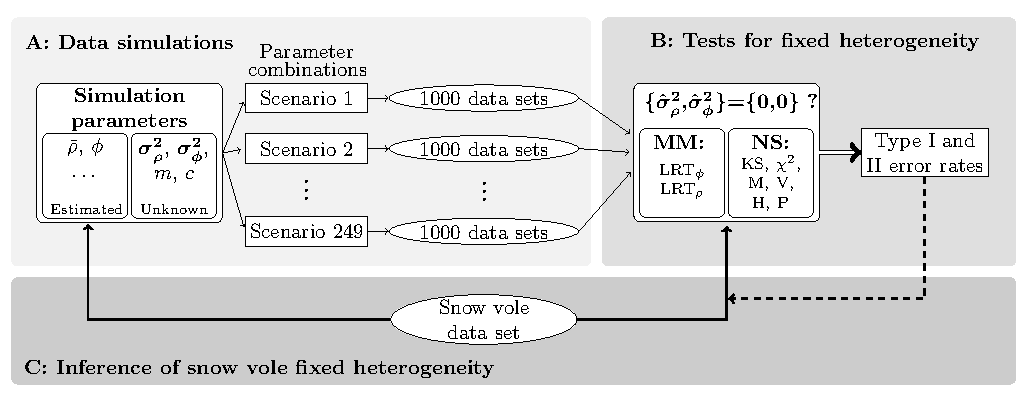
\includegraphics[width= \textwidth]{FiguresDynHet/Figure1}
		\caption{\footnotesize Illustration of the simulation and testing process. (A) Data simulation: The simulation model is parametrized using the life cycle and vital rates of a snow vole population, along with additional, unknown, parameters introducing fixed heterogeneity ($\sigma_{\phi}^2$ and $\sigma_{\rho}^2$) and dynamic heterogeneity ($m$ and $c$). Different combinations of these simulation parameters define 249 scenarios. For each scenario, 1000 data sets are simulated. (B) Tests for fixed heterogeneity: Each simulated data set is tested for the presence of fixed heterogeneity with both mixed models (\MM) using likelihood ratio tests (LRT) on survival ($\phi$) and reproduction ($\rho$), and neutral simulations (\NSM), using six different tests (see main text). Because $\sigma_{\phi}^2$ and $\sigma_{\rho}^2$ are known for each simulated data set, we can estimate the type I and type II error rates under each scenario. (C) Analysis of the snow vole data: Both \MM and \NSM are applied to the real snow vole data set, and the outcome is interpreted in the light of the estimated error rates of each test.}
	\label{figure:flow}
\end{figure}
%%%%%%%%%%%%%%%%%%%%%%%%%%%%%%%%%%%%%%%%%%%%%%%%%%%%%%%%%%%%%%%%%%%%%%%%%%%%%%%%%%%%%%%%%%%%%%%%%%%%
%%%%%%%%%%%%%%%%%%%%%%%%%%%%%%%%%%%%%%%%%%%%%%%%%%%%%%%%%%%%%%%%%%%%%%%%%%%%%%%%%%%%%%%%%%%%%%%%%%%%
%%%%%%%%%%%%%%%%%%%%%%%%%%%%%%%%%%%%%%%%%%%%%%%%%%%%%%%%%%%%%%%%%%%%%%%%%%%%%%%%%%%%%%%%%%%%%%%%%%%%
\section{Results}
Mean ARS had no effect on the error rates of any test, so we merged together the the scenarios differing only by mean ARS. Therefore, all error rates are estimated based on 3000 tests (1000 data sets per scenario, times three mean ARS values).

\subsection{Type I error rates}
In the absence of simulated individual fixed heterogeneity and non-random transition probabilities between successive stages, all tests have a low rate of null-hypothesis rejection (table \ref{table:t1error}). This means that any discrepancy between \NSM and \MM must come from a difference in type II rather than type I error rates.
\begin{table}[H]
\caption{Type I error of tests used in the \MM and \NSM approaches, when applied to data sets without underlying fixed heterogeneity and with fully random transition probabilities}
\begin{center}\scriptsize
\begin{tabular}{c c c c c c c c c c}
\toprule
& \multicolumn{2}{c}{Mixed models} & & \multicolumn{6}{c}{Neutral simulations}\\
\cmidrule{2-3} \cmidrule{5-10}%\cmidrule(r) would trim the line
& LRT$_\rho$ & LRT$_\phi$ & & KS & $\chi^2$ & H & P & M & V\\
\midrule
estimate & 0.042 			& 0.000 		& & 			0.000 & 0.021				& 0.018 			& 0.039 			& 0.000 		& 0.000\\
95\% CI & 0.039;0.054 &	0;0.001		& & 	0;0.001		& 0.016;0.027	& 0.014;0.023	& 0.033;0.047	& 0;0.001		&	0;0.001	\\
\bottomrule
\end{tabular}
\end{center}
{\scriptsize Note: Type I error rates are estimated as the proportion of simulated data sets, generated without fixed heterogeneity nor Markovian process, for which a test provides a $p$-value below 0.05. Hence, each proportion is estimated from 3,000 tests. The 95\% CI (confidence intervals) are Wilson score intervals. $\mathrm{LRT}_\rho$ and $\mathrm{LRT}_\phi$ refer to the Likelihood Ratio Tests of the variance associated with the individual random intercept in reproductive success and survival, respectively. KS refers to a Kolmogorov-Smirnov test, and $\chi^2$ to a $\chi^2$ test, both of which compare the Lifetime Reproductive Success (LRS) distribution in a focal data set to the distribution of LRS distributions obtained through neutral simulations (\NSM). The four other tests are based on the distribution of values obtained by \NSM compared to the value in the focal data set (mean (M) and variance (V) of the LRS distribution; and entropy (H) and persistence (P) of the transition matrix between successive annual reproductive successes.}
\label{table:t1error}
\end{table}

\subsection{Type II error rates}
\subsubsection{Simulations with explicit fixed heterogeneity}
\paragraph{Neutral simulations (\NSM)}
The Kolmogorov-Smirnov test comparing LRS distributions is significant for only one simulated data set (pertaining to the scenario \{$\sigma_{\rho}^2=1, \sigma_{\phi}^2=2, \bar{\rho}=50\}$) out of the 72,000 data sets with explicit fixed heterogeneity on the transformed scale. For the parameter range simulated, this test has thus effectively null power. Nevertheless, $p$-values decrease with increasing $\sigma_{\rho}^2$ and $\sigma_{\phi}^2$ (for \{$\sigma_{\rho}^2=0, \sigma_{\phi}^2=0, \bar{\rho}.\}$ $\overline{p\textrm{-value}}=0.998$, $\mathrm{SE}=0.001$; for \{$\sigma_{\rho}^2=2, \sigma_{\phi}^2=2, \bar{\rho}. $ \} $\overline{p\textrm{-value}}=0.776$, $\mathrm{SE}=0.032$), showing that the extremely low power is not the result of a complete calculation failure. Similar to the results of \cite{Plard2012}, the $\chi^2$ test is more powerful than the Kolmogorov-Smirnov test. Nevertheless, statistical power remains below 0.8 for moderately sized simulated variances, and its maximal value is 0.89 for the highest simulated variances (figure \ref{figure:VarIn}(A)).

Tests based on mean LRS are non-significant for all data sets and every scenario. The power of tests based on the variance in LRS increases with increasing $\sigma_{\phi}^2$, while the power peaks at intermediate values of simulated $\sigma_{\rho}^2$ and decreases again for higher $\sigma_{\rho}^2$ (figure \ref{figure:VarIn}(B)). The non-monotonic shape might be the result of the simultaneous increase in both the real observed-expected difference and the sampling variance: As the simulated variances go up, the LRS distribution becomes wider and flatter. Keeping the number of \NSM constant, this results in a less extensive sampling of the LRS distribution and a reduced power.

Tests based on the entropy of transition matrices display a pattern that is similar to that for $\chi^2$ tests, albeit with lower statistical power, this time peaking at 0.57 (figure \ref{figure:VarIn}(C)).
Tests based on the persistence of transition matrices have high statistical power ($\approx  0.8$) for $\sigma_{\rho}^2 \geq 1$, while increases in $\sigma_{\phi}^2$ result only in a slight increase in statistical power (figure \ref{figure:VarIn}(D)). While they reach higher statistical power than the $\chi^2$ tests, they have lower power than the $\chi^2$ at intermediate $\sigma_{\rho}^2$ values.

\paragraph{Mixed models (\MM)}
In contrast to \NSM, the power of the likelihood ratio test for ARS ($LRT_{\rho}$) is almost perfect for $\sigma_{\rho}^2 \geq 0.1$. Even though fixed heterogeneity in reproduction and survival are simulated independently, the power to detect fixed heterogeneity in reproduction is marginally influenced by the value of $\sigma_{\phi}^2$ (figure \ref{figure:VarIn}(E) and, more clearly, Appendix \ref{app:orsc} figure \ref{app:orsc}\ref{figure:VarOut}(E)). This is because a higher variance in latent survival probability increases the proportion of individuals that reach the maximal age, which provides more successive observations of reproduction and thereby increases the power to detect variance in reproductive quality. Overall, $\sigma_{\rho}^2$ is slightly underestimated ($\hat{\sigma_{\rho}^2} = 0.972 \sigma_{\rho}^2$; adjusted R$^2$=0.9997).

The $LRT_\phi$ is never significant, even for $\sigma_{\phi}^2=2$. Moreover the estimation of $\sigma_{\phi}^2$ is always close to zero (average of the median values 0.029) and does not increase with increasing $\sigma_{\phi}^2$ (slope and SE: $-0.0016 \pm 0.0006$). The failure of this model illustrates the intrinsic difficulty in estimating random effects for binary traits, especially when there are few repeated measurements per individual \parencite[e.g.][chapter 9]{Albert1984,Hosmer2013}, as is the case in our short-lived simulated animals.

\begin{figure}[H]
	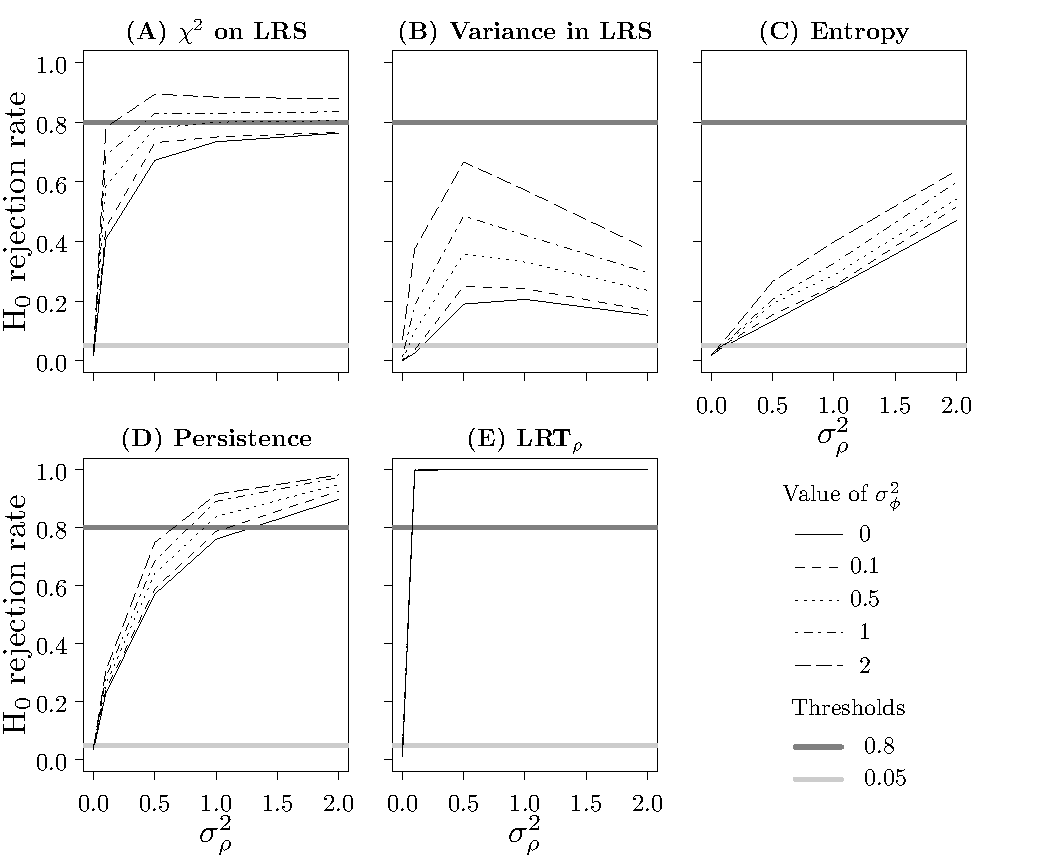
\includegraphics[width=\textwidth]{FiguresDynHet/Figure2}
		\caption{ \footnotesize Null-hypothesis rejection rates for various methods testing for the presence of fixed heterogeneity, as a function of the variance in reproductive propensity, $\sigma_{\rho}^2$, and survival propensity, $\sigma_{\phi}^2$, when these variances are introduced on the transformed scales. The methods are: (A) a $\chi^2$ test comparing the LRS distribution in a focal data set to the distribution of LRS distributions obtained through the neutral simulation approach (\NSM); tests based on proportion of values obtained by \NSM greater or equal to the value in the focal data set for (B) the variance in LRS, (C) the entropy of the transition matrix between successive annual reproductive success and (D) the persistence of this matrix; (E) a LRT for the significance of the individual random intercept in reproductive success. When $\sigma_{\rho}^2 = \sigma_{\phi}^2 = 0$, the null-hypothesis rejection rates are equal to the type I error rates, which is expected to be 0.05 (light gray line). When $\sigma_{\rho}^2 \neq 0$ or $\sigma_{\phi}^2 \neq 0$, the null-hypothesis rejection rates give (1-type II error rate), i.e. statistical power. The dark gray line indicates the 0.8 threshold. (A)-(D) are related to \NSM, (E) is related to \MM.}
	\label{figure:VarIn}
\end{figure} 	

\subsection{Simulations with a Markovian process}
Although data sets simulated using a Markovian process do not contain explicit fixed heterogeneity, both \MM and \NSM reject the null hypothesis of an absence of fixed heterogeneity in most of the cases (figure \ref{figure:Markov}).\\
The LRT$_\rho$, testing for fixed heterogeneity in ARS (based on \MM), rejects the null hypothesis with a high probability, except for the lowest values of $c$ and $m$ (figure \ref{figure:Markov}(E)). When $m > 0$, current ARS is influenced by past ARS, which in turn introduces variance in the propensity to reproduce. When $c > 0$, current survival probability is positively influenced by current ARS. As a consequence, successful reproducers live longer, resulting in more ARS values for these individuals, which improves the ability of the \MM to detect individual-level variance.
The LRT$_\phi$ is never significant for $c=0$, but rejects the null hypothesis at a high rate for $c \geq 0.5$, and this increases as $m$ increases (figure \ref{figure:Markov}(G)). This pattern was expected as $c$ controls the correlation between survival and reproduction, and indirectly makes the probability to survive in the current time step dependent on the probability to survive in the previous time step. Increasing values of $m$ further strengthen this correlation.

Both the Kolmogorov-Smirnov test on the LRS distribution, and the test based on mean LRS, are non-significant for any data set with Markovian process. Furthermore, the $\chi^2$ test rejects the null hypothesis with near certainty when $c>0$, and, when $c=0$, with probabilities going from low to moderate with increasing $m$ (figure \ref{figure:Markov}(A)). Given the absence of explicit fixed heterogeneity in these data, the $\chi^2$ test can therefore be considered to have very high type I error rates (but see the discussion).
The tests based on the variance in LRS, entropy and persistence follow a similar pattern of increasing probability of null-hypothesis rejection when $m$ and $c$ increase, but the test based on entropy does not reach a probability higher than 0.65, while the two other tests are close to 1 for the highest values of the parameters (figures \ref{figure:Markov}(B)-(D)). 

Based on these findings, it could be argued that both \MM and Plard's version of \NSM \parencite{Plard2012} have a very high type I error rate when the transitions between stages are structured. We examine this interpretation in more detail in the discussion. 
However, the rejection rate of the LRT$_\rho$ for fixed heterogeneity in ARS is drastically reduced by the inclusion of the past ARS ($\rho_{i,t-1}$) in the two mixed models that are being compared, i.e. with and without the individual random effect (compare figure \ref{figure:Markov}(E) and figure \ref{figure:Markov}(F)). The type I error rate is greater than the alpha threshold of 5\% only when both $m > 0.8$ and $c > 0$ (figure \ref{figure:Markov}(F)). Moreover, the estimates of the variance in reproductive propensity are reduced by the inclusion of $\rho_{i,t-1}$ in the models: over all the scenarios, the mean is $\hat{\sigma_{\rho}^2}=0.004$, SE=0.002, with a maximal estimate of 0.144, whereas without including $\rho_{i,t-1}$, the mean is 0.050, SE=0.008, and the maximum 0.459. The former estimate is closer to zero, i.e. the individual-level variance that is explicitly simulated.

\begin{figure}[H]
	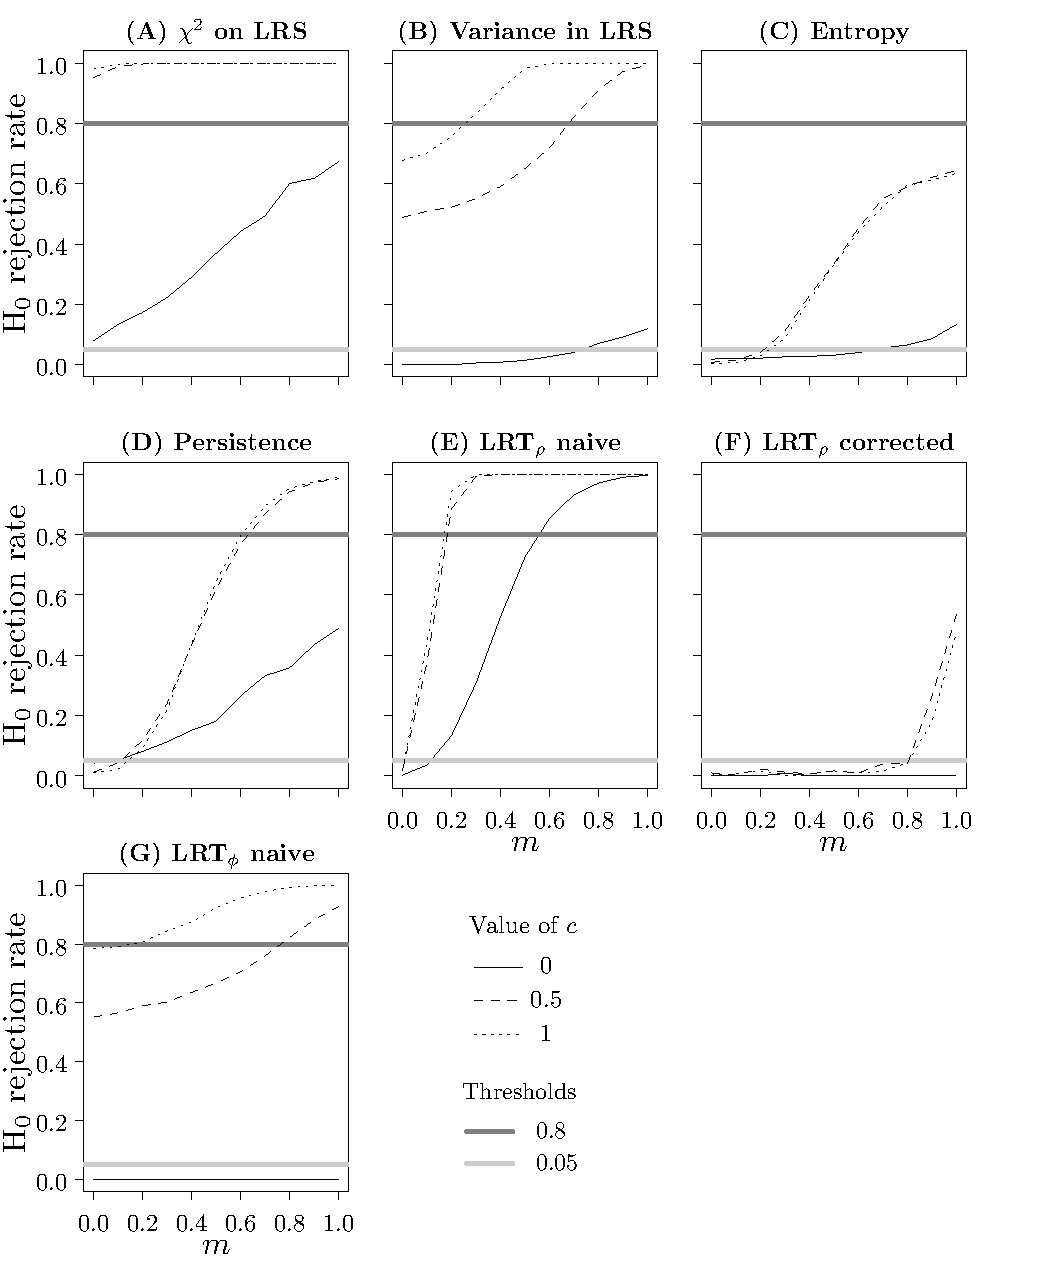
\includegraphics[width=\textwidth]{FiguresDynHet/Figure3}
	\caption{ \footnotesize Null-hypothesis rejection rates for various methods testing for the presence of fixed heterogeneity, when none is explicitly simulated, depending on the parameter $m$, controlling the structure of transitions between successive annual reproductive successes, and on the parameter $c$, controlling the dependency between survival probability and reproductive success (see the method section ``Simulations of a Markovian process'' for details). The methods are: (A) a $\chi^2$ test comparing the LRS distribution in a focal data set to the distribution of LRS distributions obtained through \NSM; tests based on proportion of values obtained by \NSM greater or equal to the value in the focal data set for (B) the variance in LRS, (C) the entropy of the transition matrix between successive annual reproductive success and (D) the persistence of this matrix; (E) a LRT for the significance of the individual random intercept in reproductive success, using models that do not account for a Markovian process, or (F) that do account for a Markovian process; (G) a LRT for the significance of the individual random intercept in survival. For survival we did not try to account for the Markovian process. Assuming that the simulated Markovian process cannot be related to fixed heterogeneity, the null-hypothesis rejection rates represent type I error rates for all values of the $c$ and the $m$ parameters. (A)-(D) are related to the \NSM framework. (E)-(G) are related to the \MM framework}
	\label{figure:Markov}
\end{figure}

%%%%%%%%%%%%%%%%%%%%%%%%%%%%%%%%%%%%%%%%%%%%%%%%%%%%%%%%%%%%%%%%%%%%%%%%%%%%%%%%%%%%%%%%%%%%%%%%%%%%
\subsection{Application to the snow vole data set}
\subsubsection{Neutral simulations (\NSM)}
For males, none of the six tests carried out within the \NSM framework are significant. Neither the LRS distribution, nor the transition matrix between successive values of ARS, are distinguishable from those generated using \NSM (table \ref{NS_table}).
For females, out of the six tests, two are significant: there is more persistence and more variance than expected under neutrality; and the test on mean LRS is close to being significant. However, the tests on the complete LRS distribution (Kolmogorov-Smirnov and $\chi^2$) are far from significant (table \ref{NS_table}). The latter is unsurprising as a graphical examination of the observed and the simulated neutral LRS distribution shows that the two distributions are almost indistinguishable (figure \ref{figure:LRS}).
According to the authors of the \NSM framework, the comparison of LRS distributions, either through a Kolmogorov-Smirnov test \parencite[in][]{Steiner2012} or a $\chi^2$ test \parencite[in][]{Plard2012}, is the gold standard when testing for the presence of fixed heterogeneity with \NSM (Steiner 2013, pers. comm. November 25th). Based on these \NSM results, there is thus no evidence for fixed heterogeneity in either of the sexes, although the results are more equivocal in females.

\begin{figure}[ht]
		%\subfigure[Females]
				{
					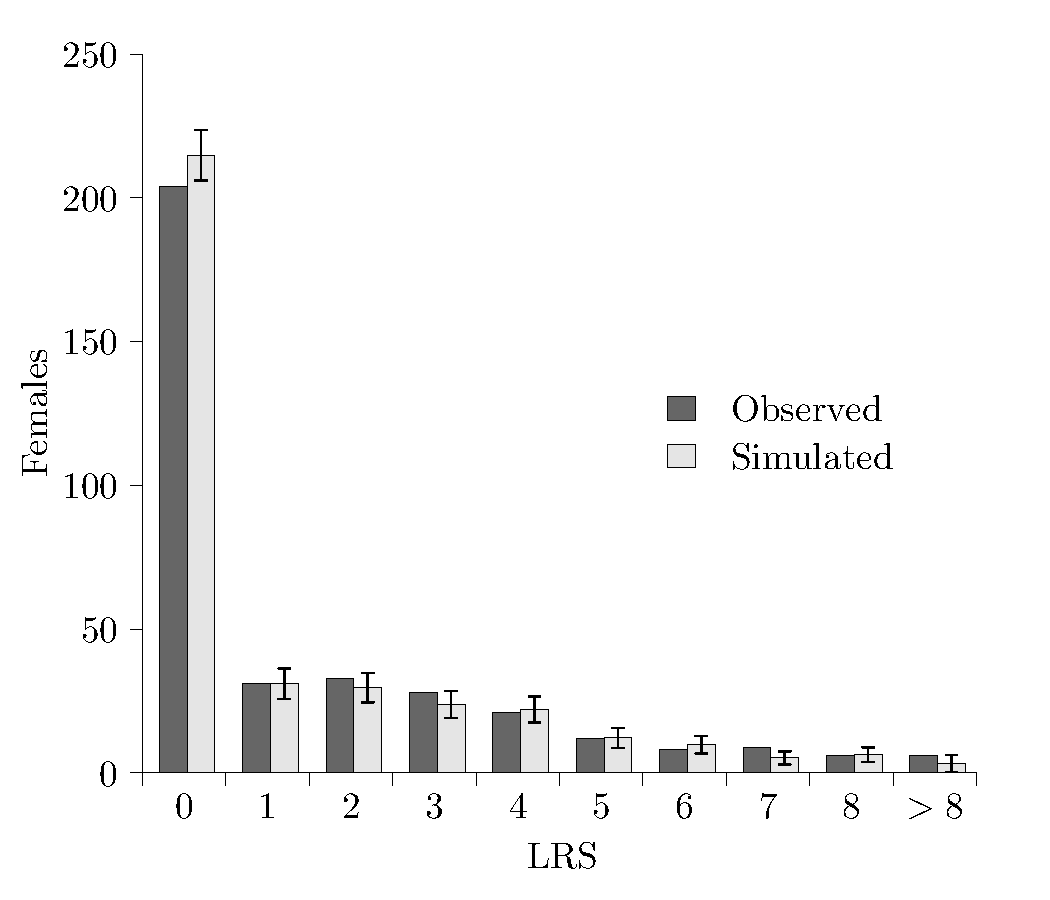
\includegraphics[width=0.5\textwidth]{FiguresDynHet/Figure4a}
					\label{figure:LRSF}
				}
		%\subfigure[Males]
				{
					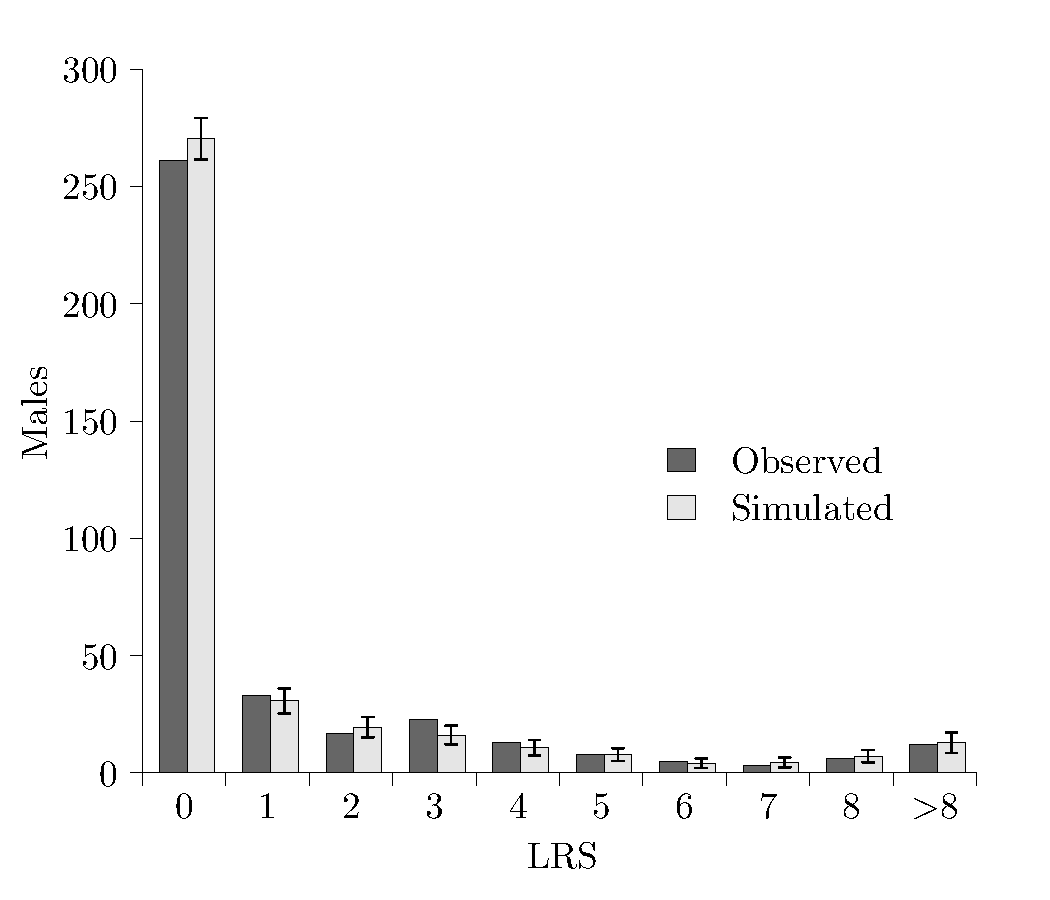
\includegraphics[width=0.5\textwidth]{FiguresDynHet/Figure4b}
					\label{figure:LRSM}
				}
\caption{ \footnotesize Distribution of lifetime reproductive success in the real snow vole data set, observed (dark bars) and simulated through 1000 neutral simulations (light bars with black error bars showing $\pm$ standard deviation), for \ref{figure:LRSF} females and \ref{figure:LRSM} males.WRONG}
				\label{figure:LRS}
\end{figure}

\begin{table}[ht]
\begin{center}
\caption{Outcomes of the various tests within the \NSM framework when applied to the real snow vole data set, for males and females separately} 
\label{NS_table}
\footnotesize
\begin{tabular}{cccccccccccc}
\toprule
\multirow{2}*{test} & \multicolumn{2}{c}{KS} & & \multicolumn{3}{c}{$\chi^2$} & & \multicolumn{1}{c}{H} & \multicolumn{1}{c}{P} & \multicolumn{1}{c}{V} & \multicolumn{1}{c}{M}\\
\cmidrule(r){2-3} \cmidrule(r){5-7} \cmidrule(r){9-12}
 & $D$ & $p$-value & & $\chi^2$ & df & $p$-value & & $p$-value & $p$-value &$p$-value &$p$-value \\
\midrule
Males  & 0.025 & 0.969 & & 8.33 & 15 & 0.909 & & 0.629 & 0.646 &0.395 & 0.378\\
Females  & 0.030 & 0.902 & & 5.50 & 8 & 0.70 & & 0.624 & \textbf{0.035} & \textbf{0.031} & 0.057 \\
\bottomrule
\end{tabular}
\end{center}
{\scriptsize Note: KS refers to the Kolmogorov-Smirnov test, and $\chi^2$ to the $\chi^2$ test, comparing the Lifetime Reproductive Success (LRS) distribution in a focal data set to the distribution of LRS distributions obtained through \NSM. The four other tests are based on the proportion of values obtained by \NSM greater than the value in the focal data set for the mean (M) and variance (V) of the LRS distribution, and for the entropy (H) and persistence (P) of the transition matrix between successive annual reproductive success. The $p$-values $ \leq $5\% are shown in bold.}
\label{table:NSCN}
\end{table}

\subsubsection*{Mixed models (\MM)} \label{sec:MMsv}
The GLMM for survival identifies significant between-years variance (5.622; 95\% CI $[1.133;13.158]$), but estimates a latent individual-level variance of 0 (95\% CI $[0;0.248]$) (see supplementary table \ref{Phi_table} for all the estimates of this model).

The GLMM for ARS estimates variances among individuals (0.371; 95\%CI $[0.151 ; 0.475]$) as well as among years (0.101; 95\%CI $[0.026 ; 0.452]$) that are different from zero, and LRTs for both variances are highly significant. The random effect accounting for overdispersion does not significantly differ from zero, although its bootstrapped confidence interval includes positive values (table \ref{Rho_table} for all the estimates of this model). When the individual random effect is not included, this overdispersion variance is highly significant, and the sum of squared Pearson residuals divided by the estimated residual degrees of freedom is approximately 2, while it falls to 1 with individual as a random effect. The estimation of residual degrees of freedom in GLMMs is a complex issue \parencite{Pinheiro2000}, but this approach seems to indicate that the overdispersion in the distribution is largely due to differences between individuals.

Excluding individuals reproducing for the first time, we fitted a GLMM that includes the previous reproductive success $\mathrm{ARS}_{t-1}$ and sex as fixed effects, and year as the only random effect. This model indicates a significant positive relationship between successive values of ARS (slope=0.0949; $\mathrm{SE}=0.0213$; $p$-value=$8 \times 10^{-06}$). Nevertheless, adding individual as a random effect greatly improved the fit of the model ($\Delta \mathrm{AIC}=87$; LRT: $p$-value $<10^{-16}$), providing evidence for the existence of significant individual-level variance ($\hat{\sigma_{id}^2}=0.341$, bootstrapped 95\% CI $[0.189;0.453]$). Including $\mathrm{ARS}_{t-1}$ had little effect on the estimate of $\hat{\sigma_{id}^2}$ (see table \ref{Rho_table}), but now $\mathrm{ARS}_{t-1}$ no longer reached significance (slope=0.0210; $\mathrm{SE}=0.0275$; $p$-value=0.445).

Finally, the latent correlation between the propensities to survive and to reproduce was estimated as 0.32 (95\% CI [-0.68;0.97]) and appears in the best model selected by DIC (see Appendix \ref{ap:cor}).

%%%%%%%%%%%%%%%%%%%%%%%%%%%%%%%%%%%%%%%%%%%%%%%%%%%%%%%%%%%%%%%%%%%%%%%%%%%%%%%%%%%%%%%%%%%%%%%%%%%%
%%%%%%%%%%%%%%%%%%%%%%%%%%%%%%%%%%%%%%%%%%%%%%%%%%%%%%%%%%%%%%%%%%%%%%%%%%%%%%%%%%%%%%%%%%%%%%%%%%%%
%%%%%%%%%%%%%%%%%%%%%%%%%%%%%%%%%%%%%%%%%%%%%%%%%%%%%%%%%%%%%%%%%%%%%%%%%%%%%%%%%%%%%%%%%%%%%%%%%%%%

%%%%%%%%%%%%%%%%%%%%%%%%%%%%%%%%%%%%%%%%%%%%%%%%%%%%%%%%%%%%%%%%%%%%%%%%%%%%%%%%%%%%%%%%%%%%%%%%%%%%
%%%%%%%%%%%%%%%%%%%%%%%%%%%%%%%%%%%%%%%%%%%%%%%%%%%%%%%%%%%%%%%%%%%%%%%%%%%%%%%%%%%%%%%%%%%%%%%%%%%%
%%%%%%%%%%%%%%%%%%%%%%%%%%%%%%%%%%%%%%%%%%%%%%%%%%%%%%%%%%%%%%%%%%%%%%%%%%%%%%%%%%%%%%%%%%%%%%%%%%%%
\section{Discussion}
\subsection{Overview}
Based on extensive simulations, we have shown that in the presence of fixed heterogeneity, \NSM have much less statistical power than \MM, even when the model simulating the data does not match the structure assumed by the \MM. In particular the Kolmogorov-Smirnov test, advocated in the earlier version of \NSM, has virtually no statistical power. In contrast, \MM have low type I error rates and are not misled by the presence of dynamic heterogeneity, which in all data sets is non-zero if it is measured as entropy \parencite{Tuljapurkar2009}. This finding directly contradicts the claim ``[\dots] that random effect models will always detect unobservable fixed effects'' \cite{Steiner2010}.
Second, in the absence of fixed heterogeneity, Markovian transitions between successive reproductive success and survival probabilities can induce high type I error rates, both in \MM and \NSM sensu \cite{Plard2012}. However, inclusion of previous reproductive success in the \MM for reproduction substantially reduces these errors.
Third, when applied to a real data set for a wild population of snow voles, \NSM only detect ambiguous deviations from neutrality and only for females. Moreover, the main tests of the framework, based on the total distribution of LRS, fail to reject the null hypothesis in both sexes. In striking contrast, \MM show strong evidence for individual latent variance in reproductive success, even when a Markovian process is accounted for. In addition, \MM give some indication of the presence of individual latent variance in survival, and of a positive correlation between survival and reproduction. However, the latter two parameters are estimated with substantial uncertainty.

\subsection{Use of simulations}
Testing methods on simulated data can be difficult because the specific simulation process used can differently match the assumptions and structures of the different methods. We tried to overcome this issue by using three different simulation models. 
Moreover, the rejection rates of \MM and \NSM observed in our simulations are similar to those observed when the methods are applied to real data. Indeed, in the present work we applied both methods to a snow vole data set and found that the \MM approach detected individual fixed heterogeneity, while the \NSM approach did not detect a significant deviation from the neutral expectation. This was also the case for the other data sets to which both methods were applied (\MM by \cite{Cam2013}; \NSM by \cite{Steiner2010}). On the whole we are aware of only a single case in which \NSM led to the rejection of neutrality  \parencite{Plard2012}, whereas \MM commonly find evidence for significant individual fixed heterogeneity, either by estimation of positive variance components, model selection \parencite{Cam2013} or posterior predictive checks \parencite{Chambert2014}. Although there is some possibility of publication bias, this pattern is consistent with our power analysis.

\subsection{Low power of Neutral Simulations}
The low power of \NSM probably stems from the fact that they aggregate data on vital rates, and that they do so twice: first over the lifetime of individuals, and then they aggregate individuals into population-level statistics. Thereby they first discard the repeatability of individuals, which has been shown to blur heritable differences among individuals \parencite{Vaupel1988}. Second, population-level statistics can be produced by an infinite number of different mixtures of individual types (for instance, a mean probability of 0.5 can be the result of a population consisting only of individuals with a latent probability of 0.5, or from a uniform distribution of individual probabilities between 0 and 1). Therefore, some patterns of among-individual differences are indistinguishable at the population level. Individual-level data are naturally better at identifying the causes of variation at that level \parencite{Cluttonbrock2010}, and the ability to use non-aggregated data, for instance longitudinal information on marked individuals, further increases this power \parencite{Brooks2013}. While a method such as Plard's \NSM could be valuable in the absence of such data, alternative methods making use of non-aggregated information, such as \MM, should be preferred whenever possible.

Importantly, within a strict null-hypothesis testing framework, the failure to reject a null hypothesis cannot be interpreted as a proof of the null hypothesis. The absence of significance in most implementations of the \NSM \parencite{Steiner2010,Orzack2011,Tuljapurkar2009,Plard2012} is therefore not informative with respect to the presence and the biological significance of fixed heterogeneity. The null-hypothesis testing framework can partially be relaxed by an a priori power analysis. Although comparisons of simulated data sets with and without heterogeneity were indeed presented in \cite{Steiner2012}, there fixed heterogeneity (assumed to be genetic) was modeled as two groups of homogeneous individuals, which except for clonal organisms is biologically unrealistic. In addition, the absence of significant differences between the data sets with and without fixed heterogeneity was not interpreted as a sign of a lack of statistical power, but as evidence that fixed heterogeneity has little effect on LRS distributions. 

\subsection{Effect of Markovian transitions}
When no fixed heterogeneity was explicitly simulated, both \MM and \NSM rejected the null hypothesis that fixed heterogeneity is absent. This was to be expected for \MM, given that Markovian transitions mimic individual-level variance, and \MM do not model population-level transition probabilities. It is more surprising that also \NSM had a high rate of false positives. However, we here used the ``full random model'' re-formulation of \NSM \parencite{Plard2012}, and not the ``full dynamic model'' \parencite{Tuljapurkar2009}. The latter simulates individual trajectories using a Markovian process, similar to the way data sets were simulated here, while the former simulates individual trajectories without taking into account the previous state.
Hence, ``full dynamic \NSM'' would not reject the null hypothesis, and one could consider this in this case to be correct. However, as latent individual quality will necessarily produce a pattern that is consistent with a Markovian process, this formulation does not allow for a complete separation of fixed and dynamic heterogeneity \parencite{Plard2012}.
Observing a Markovian process is therefore in itself not informative with respect to the mechanisms shaping life histories. Hence, although they have a low type I error rate, ``full dynamic \NSM'' always have low statistical power. 

We acknowledge that a Markovian process that is not due to fixed differences between individuals does mimic fixed heterogeneity, and thereby can bias estimates of between-individual variance based on full random \NSM and on \MM. Therefore, a naive \MM detects individual-level heterogeneity, irrespective of whether it is due to a population-level Markovian process or to individual-level differences. However, the type I error of \MM can be substantially reduced by including previous reproductive success in the model \parencite{Rotella2008, Cam2013}. Although this is not a universal solution that accounts for all confounding factors, it highlights the flexibility of the \MM framework, which allows for the incorporation of any factor that is perceived as potentially confounding based on knowledge of the study system. 

\subsection{Genetic variation as a source of fixed heterogeneity}
In cases where the evidence for the presence of fixed heterogeneity is equivocal, for instance because the effects of Markovian processes and individual-level fixed differences are confounded, the use of genetic information and quantitative genetic methods has the potential to tease apart latent genetic quality from other sources of performance persistence, including stochastic transitions.
Indeed, although other sources of variation may also generate fixed heterogeneity, the existence of significant additive genetic variation implies significant fixed heterogeneity, by definition determined at fertilization.
Interestingly, estimates of additive genetic variation for fitness components are often large, even in small populations \parencite[for reviews see][]{Mousseau1987, Postma2014}. As a matter of fact, when standardized by the mean (i.e. evolvability) rather than the variance (i.e. heritability), fitness components appear to have higher additive genetic variation than other types of traits \parencite{Hansen2011,Postma2014}. In addition to our findings, this provides further support for fixed heterogeneity being more common than suggested by \NSM.

\subsection{Interpretation of the snow vole results}
Because they are similar in structure, our simulated data sets can shed light on the results from the analysis of the real snow vole data set. For example, it is  unsurprising that the \MM fails to detect individual heterogeneity in snow vole survival probabilities. The LRT$_\phi$ has no statistical power for simulated data sets with simulated $\sigma_{\phi}^2 \leq 2$, while confidence and credibility intervals indicate that the possible values of $\sigma_{\phi}^2$ lay between 0 and 1 at most (supplementary tables \ref{Phi_table} and \ref{MCMCtable}).  
Unlike heterogeneity in individual survival probability, heterogeneity in individual reproductive success is easily detected and quantified by \MM applied to simulated data sets (figure \ref{figure:VarIn}(E)). Accordingly, the analysis of the real data set identifies an individual variance in the propensity to reproduce that is significantly different from zero, and is estimated to be more than three time larger than the variance among years. Finally, given the estimate of the variance $\sigma_{\rho}^2$, we can get an estimate of the statistical power of the other tests to detect fixed heterogeneity in the real snow vole data set: a significant test seems possible for the $\chi^2$ test (figure \ref{figure:VarIn}(A)), but quite unlikely for the test based on entropy (figure \ref{figure:VarIn}(C)).

A positive correlation between individual-level variation in reproduction and survival would provide further support for fixed heterogeneity. However, as mentioned above, the estimation of individual-level variance in survival is difficult because this is a binary trait, and because due to their short lifespan there are few observations per individual. Hence there is a lot of uncertainty in the estimation of this correlation parameter. Nevertheless, the most likely values are positive (Appendix \ref{ap:cor}).

\subsection{Fixed heterogeneity and the concept of fitness}
The debate surrounding the biological significance of fixed heterogeneity appears to stem at least partly from different concepts of fitness. On the one hand, proponents of the neutral theory of life histories consider fitness to be a property of a category of individuals, and consider variation in reproductive success among individuals to be mostly due to dynamic heterogeneity, rather than due to variation in latent individual properties \parencite{Steiner2012}. On the other hand, researchers in the field of evolutionary ecology often see fitness as a latent property of individuals \parencite{Cam2000}, that is, an expected value defined at the individual level that cannot be measured directly \parencite{Brandon1984,Price1996,Krimbas2004}. 
As the mean value of a group is also the expected value of an individual belonging to this group, the two views are not fundamentally different. In sexual organisms however, each individual is unique, which makes it difficult to assign it to a hypothetical group made of identical individuals. If stochastic variation underlies most of the realized reproductive success and there are no fitness differences between individuals, as adherents of the neutral theory of life histories advocate, then it is useless to define fitness at the individual level. However, if there exists significant fixed heterogeneity, individual performances carry some information about their latent properties, for example due to their genetic makeup. In the presence of fixed heterogeneity it therefore seems useful to use an individual-level definition of fitness, differing from both group-level fitness and realized reproductive success.

\section{Conclusions}
Using extensive simulations, we have demonstrated that \NSM are uninformative with respect to the biological significance of fixed heterogeneity.
Based on the work of \cite{Plard2012} and our power analysis, we conclude that the observation of a Markovian process in stage-transition probabilities does in itself not provide any biological insights. Within the \NSM framework, the full random model \parencite{Plard2012} should be preferred over the full dynamic model \parencite{Tuljapurkar2009}, and the $\chi^2$ test should be preferred over the Kolmogorov-Smirnov test. In addition, any use of \NSM should be complemented by an a priori power analysis, or otherwise be restricted to a strict null-hypothesis testing framework, where failure to reject the null hypothesis does not allow any conclusions regarding the null hypothesis being true, and/or the alternative hypothesis false. 
However, even when these improvements are included in the \NSM framework, we recommend that its use is restricted to data sets where individuals are not identified. 

Instead, we show that \MM are more powerful, but not more susceptible to type I error. Although \MM can be mislead by confounding factors, given a good knowledge of the biological system, it is possible to account for these confounding factors, in which case \MM have a very low type I error rate. 

Finally, the confrontation of our power analysis with the analysis of the real snow vole data set supports the presence of fixed heterogeneity in fitness components in this population. Further research is being carried out to identify what traits can be related to this latent heterogeneity, and how genetic and maternal effects shape these differences.

On the whole, this work supports the idea that fixed heterogeneity is more common than suggested by the studies based on \NSM. 

\section{Acknowledgments}
We thank Arpat Ozgul, Yannis Michalakis, Benjamin M. Bolker, Gordon A. Fox and an anonymous reviewer for helpful comments on this manuscript. Thanks to Ulrich K. Steiner for discussions on an earlier version of this work and for help with the implementation of neutral simulations. Thanks also to Lukas Keller, Josh Van Buskirk and Pirmin Nietlisbach for inspiring discussions on this topic. The snow vole monitoring was authorized by the \textit{Amt f\"{u}r Lebensmittelsicherheit und Tiergesundheit}, Chur, Switzerland. Funding was provided by the Swiss National Science Foundation project grant (\verb|31003A_141110|). 

%%%%%%%%%%%%%%%%%%%%%%%%%%%%%%%%%%%%%%%%%%%%%%%%%%%%%%%%%%%%%%%%%%%%%%%%%%%%%%%
%%%%%%%%%%%%%%%%%%%%%%%%%%%%%%%%%%%%%%%%%%%%%%%%%%%%%%%%%%%%%%%%%%%%%%%%%%%%%%%
\printbibliography[heading=subbibliography]

%%%%%%%%%%%%%%%%%%%%%%%%%%%%%%%%%%%%%%%%%%%%%%%%%%%%%%%%%%%%%%%%%%%%%%%%%%%%%%%
%%%%%%%%%%%%%%%%%%%%%%%%%%%%%%%%%%%%%%%%%%%%%%%%%%%%%%%%%%%%%%%%%%%%%%%%%%%%%%%
\newpage
\textbf{\LARGE{Supplementary information}}

\section{Checking the properties of the data sets}\label{ap:chpro}
The following Generalized Linear Models were fitted to the simulated data sets in order to test whether the data set properties matched the parameters used to generate them:

\begin{subequations}\label{eq:check}
\begin{align}
&\mathrm{logit}(\phi_{i,t})=\mu_{\phi}+\mathrm{Age}_{i,t}\label{eq:checkPA}\text{ ; using a binomial error structure}\\
&\mathrm{logit}(\phi_{i,t})=\mu_{\phi}+\rho_{i,t}\label{eq:checkPR}\text{ ; using a binomial error structure}\\
&\mathrm{log}(\rho_{i,t}) =\mu_{\rho}+ \rho_{i,t-1}\label{eq:checkRR}\text{ ; using a quasi-Poisson error structure}\\
&\mathrm{log}(\rho_{i,t}) =\mu_{\rho}+ \mathrm{Age}_{i,t}\label{eq:checkRA}\text{ ; using a quasi-Poisson error structure}
\end{align}
\end{subequations}

These were used to check that survival depended on age \eqref{eq:checkPA}, that survival depended on annual reproductive success only when that was required \eqref{eq:checkPR}, that ARS depended on previous reproductive attempts only when fixed heterogeneity for reproductive success or Markovian reproduction was simulated \eqref{eq:checkRR} and that ARS of adults was not age-dependent \eqref{eq:checkRA}. The simulated data had all the expected properties. Furthermore, we never found a significant association between reproduction and survival. This goes against the claim made in \cite{Steiner2010} that dynamic heterogeneity alone can generate a positive association between reproduction and survival.

Instead, we argue here that the findings on which they base their claim reflects their use of reproductive stage-specific survival in their \NSM, and reproduction and survival being positively correlated in the source data \parencite{Cam2002}. Hence, it is not the random transitions themselves that are responsible for the positive association, but the positively associated stage-specific probabilities of survival and reproduction. The origin of the latter remains unexplained, but is consistent with variation in latent fitness among individuals.

\section{Optimal number of neutral simulations per data set.}\label{ap:opnum}
The neutral simulation approach (\NSM) is computationally intensive: as the focal population consists of 10 cohorts of 100 individuals, performing 1000 neutral simulations (i.e. simulating 1000 hypothetical populations), requires 1,000,000 individual trajectories to be simulated for every simulated data set (and 75,000,000,000 individual trajectories for the complete study). To minimize computational time, we determined the number of neutral simulations per simulated data set beyond which statistical power did not change. Out of the six tests mentioned above, only $\chi^2$ tests on LRS distributions are sensitive to the number of neutral simulations; while $\chi^2$ tests based on 1000 neutral simulations differ from those based on 100 neutral simulations ($\Delta \mathrm{power}_{1000-100}$=-0.067, se=0.033), the tests based on 100,000 neutral simulations do not have more statistical power than those based on 1000 neutral simulations ($\Delta \mathrm{power}_{100,000-1000}$=-0.031, se=0.033), and the correlation of the statistical power across scenarios is high ($R^2=0.92$).
Accordingly, each simulated data set was analyzed using 1000 neutral simulations. Note that the fact that in this case statistical power plateaus already above 1000 neutral simulations is the result of the relatively short lifespan of the simulated animals, which allows for a quick exploration of all the possible individual trajectories. 

\section{Selection for latent quality}\label{ap:sel}

As outlined in the main document, we simulated fixed heterogeneity by attributing to each individual $i$ a fixed quality for annual reproductive success ($q_{\rho, i}$) and a fixed quality as survivor ($q_{\phi,i}$). These two kind of individual qualities are normally distributed, with mean zero and variance $\sigma_{\rho}^2$ and $\sigma_{\phi}^2$, respectively. The selection acting on, or due to, this variation in latent individual qualities for reproduction and for survival was measured as the individual-level covariance between the qualities and a proxy for fitness ($\omega$): relative lifetime reproductive success \parencite{Robertson1966}.

The selection coefficients increase with increasing variance in individual latent qualities, both for reproduction (figure \ref{ap:sel}\ref{figure:qua:rho}) and for survival (figure \ref{ap:sel}\ref{figure:qua:phi}). This confirms that the heterogeneity simulated is non-neutral. 

\begin{figure}[H]

%	\subfigure[Reproduction quality]
		{
			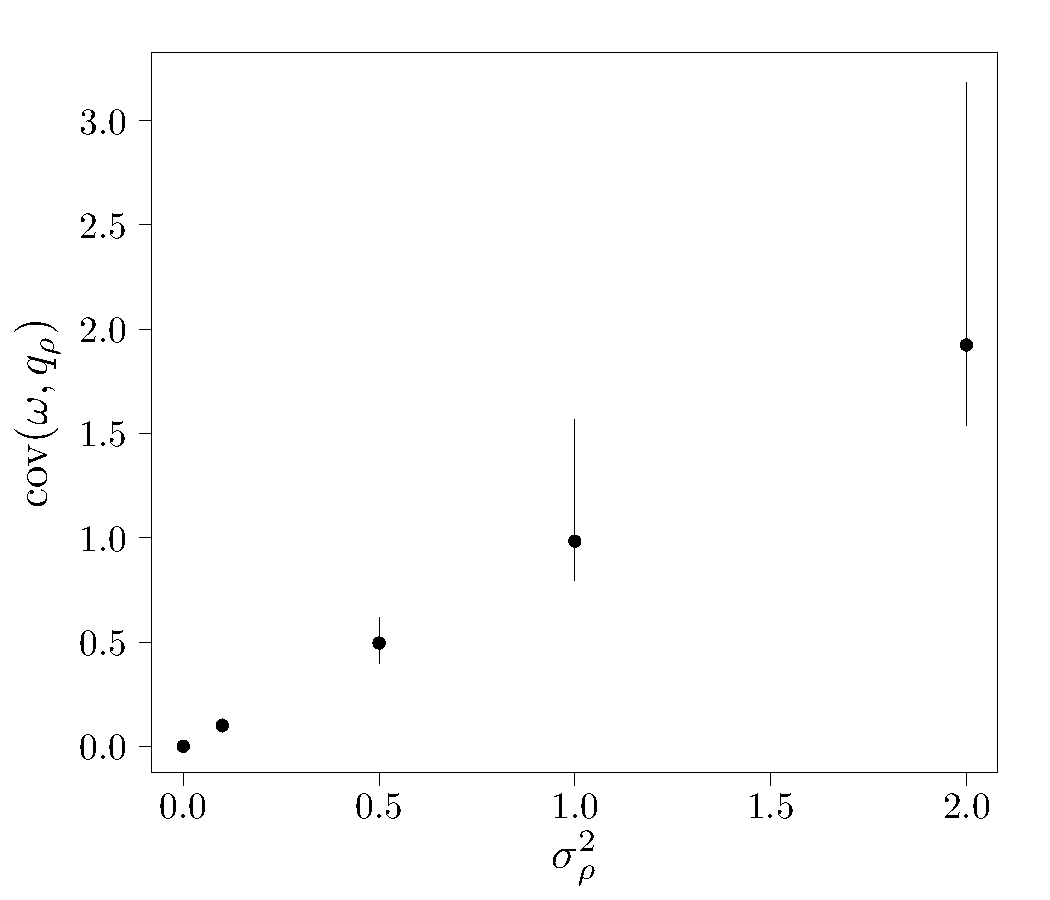
\includegraphics[width=0.5\textwidth]{FiguresDynHet/Figure5a}
			\label{figure:qua:rho}
		}
	%\subfigure[Survival quality]
		{
			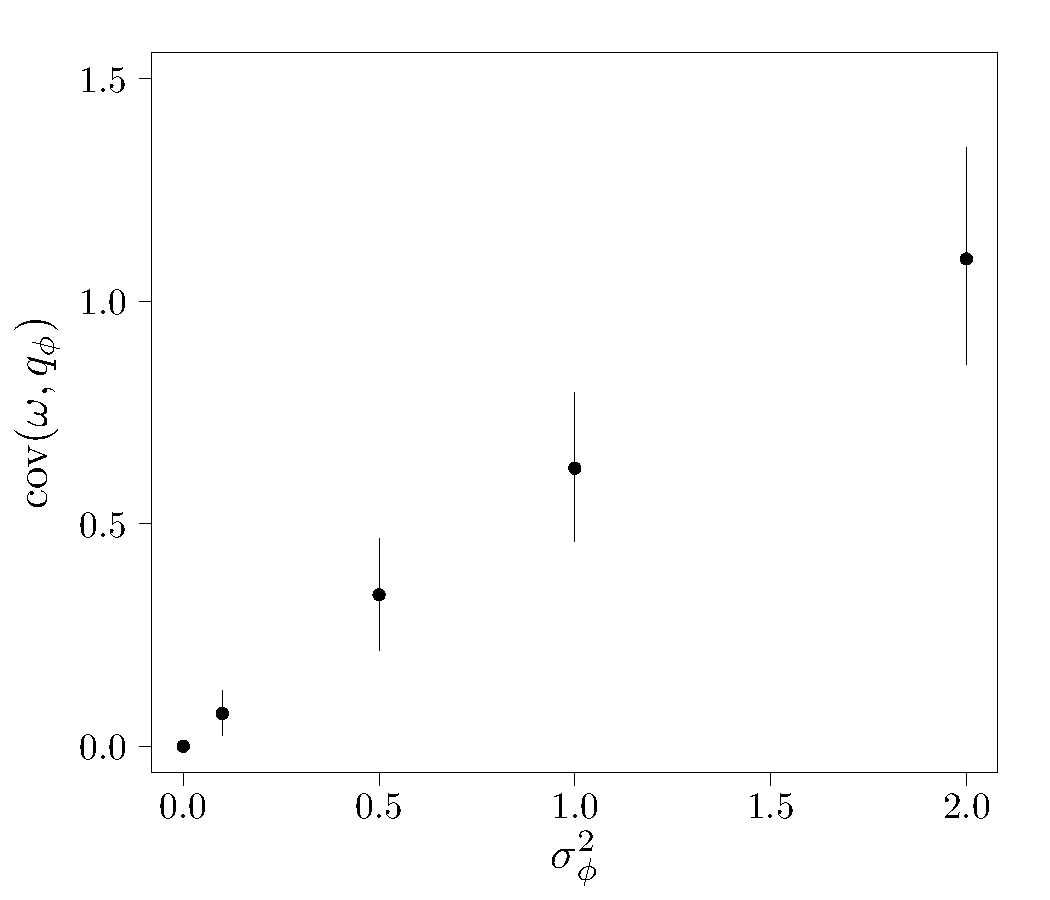
\includegraphics[width=0.5\textwidth]{FiguresDynHet/Figure5b}
			\label{figure:qua:phi}
		}
	\caption{ Appendix C \footnotesize Strength of selection on individual fixed qualities for survival and reproduction, as a function of the expected variance in these qualities. Strength of selection was measured as the individual-level covariance between the qualities and a proxy for fitness ($\omega$): relative lifetime reproductive success;  %\subref{figure:qua:rho} 
	for reproduction quality and %\subref{figure:qua:phi} 
	for survival quality. Vertical bars show the 95\% interval of the estimate distributions.}
	\label{figure:qua}
\end{figure}

\section{Simulating fixed heterogeneity on the original scale}\label{app:orsc}
It could be argued that the superior statistical power of the  $\mathrm{LRT}_{\rho}$ is the result of the simulation process used to introduce fixed heterogeneity has the same structure as the \MM estimating it. To address this, additional simulations were performed in which individual reproductive success and survival probability depended on their qualities on the original scale rather than on a transformed scale. Otherwise simulations were similar to those where fixed heterogeneity was introduced on the transformed scale. To this end, the reproductive success and survival of an individual $i$, at time $t$, are drawn from

\begin{subequations}\label{eq:varout}
\begin{align}
\rho_{i,t} &\sim \text{{\fontfamily{pzc}\selectfont P }}(\mu_{\rho}+q_{\rho,i})\\
\text{and } \phi_{i,t} &\sim \text{{\fontfamily{pzc}\selectfont B }}(\mu_{\phi}+\beta_{age}+q_{\phi,i}).
\end{align}
\end{subequations}


Although when the variance in quality for reproduction is included on the original, non-transformed, scale, mean reproductive success ($\overline{\mathrm{ARS}}$) has a dramatic negative influence on the power of the different tests, the hierarchy in the performance of the different tests does not change across the values of mean reproductive success. Therefore, we chose to present the results with pooled $\overline{\mathrm{ARS}}$ only (figure \ref{figure:VarOut})
Furthermore, it should be noted that although the $\sigma_{\rho}^2$ parameter values are the same in this section as in the previous one (0,0.1,0.5,1 and 2), they correspond to much smaller realized variances, as the variance is introduced on the original scale and not on a log-scale as previously. For correspondence between the variances on the two scales, see table \ref{table:Vlink}. 

\begin{table}[h]
\caption{Realized variance on the log scale as a function of variance introduced on the original scale ($\sigma_{\rho}^2$) and  mean reproductive success ($\overline{\rho}$)}
\begin{center}
\footnotesize
\begin{tabular}{c c c c c c}
\toprule
\multirow{2}{*}{$\overline{\mathrm{ARS}}$} &\multicolumn{5}{c}{$\sigma_{\rho}^2$ on original scale}\\
\cmidrule(r){2-6}
 & 0 & 0.1 & 0.5 & 1 & 2\\
\midrule
3 & 0 & 0.01143 & 0.06649 & 0.16947 & 0.39091 \\
10 & 0 & 0.00100 & 0.00506 & 0.01027 & 0.02108 \\
50 & 0 & 0.00004 & 0.00020 & 0.00040 & 0.00079 \\
\bottomrule
\end{tabular}
\end{center}
\label{table:Vlink}

{\scriptsize Note: Each realized variance was estimated from the variance of the log of 1,000,000 draws from a normal distribution of mean $\overline{\rho}$ and variance $\sigma_{\rho}^2$.}
\end{table}

\begin{figure}[H]
		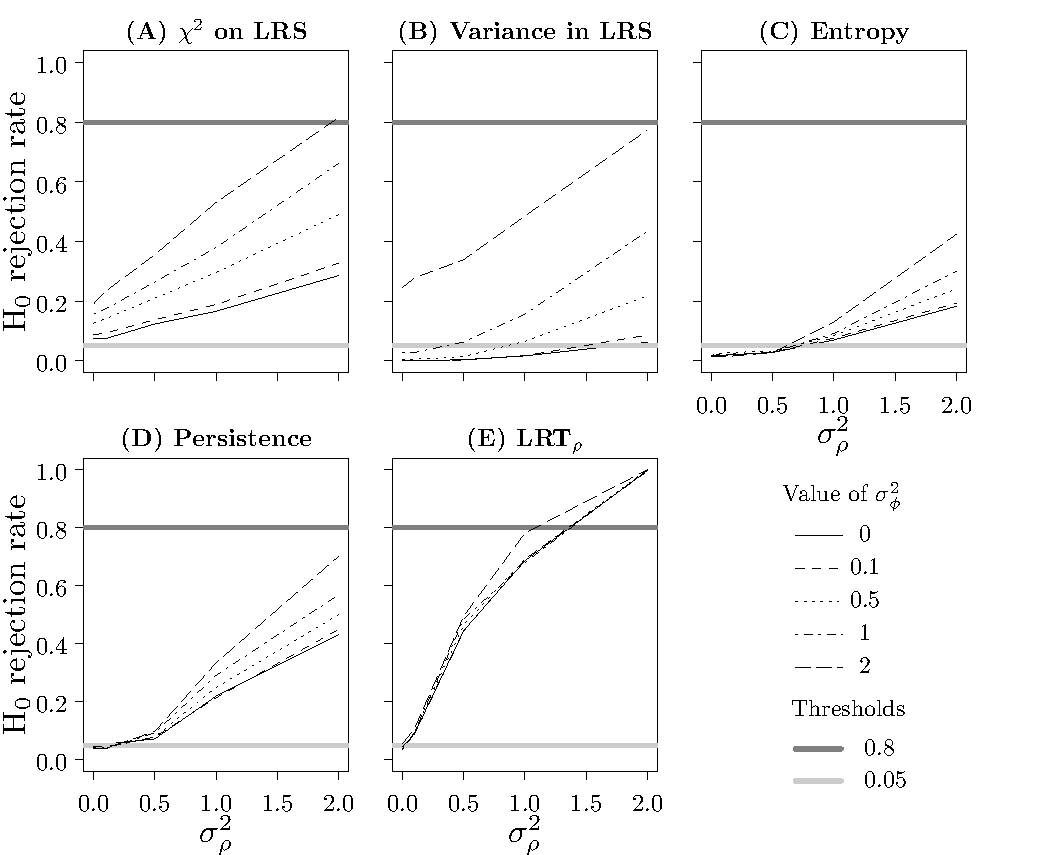
\includegraphics[width=\textwidth]{FiguresDynHet/Figure6}
	\caption{Appendix D \footnotesize Null-hypothesis rejection rates for various methods testing for the presence of fixed heterogeneity, depending on the variance in reproductive propensity, $\sigma_{\rho}^2$, and on the variance in survival propensity, $\sigma_{\phi}^2$, when these variances are introduced on the original scales. The methods are: (A) a $\chi^2$ test comparing the Lifetime Reproductive Success (LRS) distribution in a focal data set to the distribution of LRS distributions obtained through the neutral simulation approach (\NSM); tests based on proportion of values obtained by \NSM greater or equal to the value in the focal data set for (B) the variance in LRS, (C) the entropy of the transition matrix between successive annual reproductive success and (D) the persistence of this matrix; (E) a Likelihood Ratio Test for the significance of the individual random intercept in reproductive success. When $\sigma_{\rho}^2 = \sigma_{\phi}^2 = 0$, the null-hypothesis rejection rates are equal to the type I error rates, which is expected to be 0.05 (light gray line). When $\sigma_{\rho}^2 \neq 0$ or $\sigma_{\phi}^2 \neq 0$, the null-hypothesis rejection rates give (1-type II error rate), i.e. statistical power, which should be above 0.8 (dark gray line). (A)-(D) are related to \NSM, (E) is related to \MM.}	
	\label{figure:VarOut}
\end{figure}

\section{The snow vole population}\label{ap:snv}
\setcounter{table}{0}
\setcounter{equation}{0}
\setcounter{figure}{0}
A snow vole population, located in the central eastern Alps near Churwalden, Switzerland ($46^{\circ}$48' N, $9^{\circ}$34' E) at 2000m above sea level, has been monitored continuously since 2006. Analyses presented here are based on data collected until 2013. The study site consists of scree, which is the favourite habitat of the species, interspersed by patches of alpine meadows and surrounded by forest and larger meadows, which are not suitable habitats \parencite{Janeau1997}. Four trapping nights are necessary for sampling the complete area. Trapping throughout the whole study area took place two (in one year), three (in three years) or five times (in four years), between late May and mid-October. 

Unknown individuals were marked with a subcutaneous passive transponder (PIT, ISO transponder, Tierchip Dasmann, Tecklenburg) and an ear tissue sample was taken (maximum 2mm diameter, Thumb Type Punch, Harvard Apparatus) and stored in 90\% ethanol at $-20^{\circ}\mathrm{C}$. DNA extracted from the tissue samples was genotyped for 18 specific autosomal microsatellites developed for this population \parencite{Wandeler2008}, and the \textit{Sry} locus was genotyped in order to confirm the sex of all individuals. To identify cases of PIT loss as well as recaptures of juveniles initially too light for PIT injection, an identity analysis in CERVUS v.3.0 \parencite{Marshall1998} was carried out to detect resampled individuals.
Parentage was assigned to all juveniles and all first-time captured adults by simultaneously reconstructing parentage and sibship using the R package MasterBayes \parencite{Hadfield2006}. Analyses were performed for each year separately assuming polygamy for males and females and a uniform genotyping error rate of 0.5\% for all 18 loci. Parentage was assigned using a parental pool of all adults present in the examined year and the previous year. Because some rare first year individuals reproduce at the end of the season, as evidenced by the observation of pregnant and lactating first year individuals, the ``juveniles'' were also included in the parental pool of a second analysis excluding parent-offspring mating. Thereby eight additional parentage links could be identified. There were no inconsistencies between the reconstructed pedigree and the transmission of two sex-specific markers: a polymorphic Y-chromosome locus developed for this population \parencite{Wandeler2011} and a fragment of the mitochondrial DNA control region, amplified using vole specific primers \parencite{Haring2000}. This pedigree was used to measure annual and lifetime reproductive success.

Apparent year-to-year survival could be obtained without mark-recapture modeling as the recapture probability on a given year was virtually 1: no animal was not captured in a year but captured later, and no animal was ever found to be a parent of a juvenile in a year when it had not been captured. This is not surprising since mark-recapture modeling within years estimated a between-occasion recapture probability of 0.924 (SE 0.012) for adults and of 0.814 (SE 0.030) for juveniles.


\section{Univariate models of survival and reproduction in the snow vole population}\label{ap:Uni}

The following two tables (\ref{Phi_table} and \ref{Rho_table}) present all the estimates from the univariate models used to estimate the individual-level variance in survival and reproductive propensities for the snow vole population.
% latex table generated in R 3.1.2 by xtable 1.7-4 package
% Wed Nov 12 18:14:03 2014
\begin{table}[H]
\begin{center}
\caption{Estimates of coefficient of the mixed model for survival in the real snow vole data set}\label{Phi_table}
\footnotesize
\begin{tabular}{ccccc}
  \toprule
 & Estimate & SE & $p$-value & Bootstrap 95\% CI  \\ 
  \midrule
	Random effects:\\
$\sigma_{id}^2$ & 0.000 & - & 0.500 & [0;0.248] \\ 
  $\sigma_{year}^2$ & 5.622 & - & $<10^{-16}$ & [1.133;13.158] \\ 
	\\
   Fixed effects:\\
intercept & -1.754 & 0.830 & 0.035 & [-3.393;-0.111] \\ 
  age (Juvenile) & 1.841 & 0.230 & 0.000 & [1.369;2.411] \\ 
  sex (Male) & 0.306 & 0.295 & 0.300 & [-0.389;0.93] \\ 
  age:sex & -0.705 & 0.333 & 0.034 & [-1.449;0.091] \\ 
   \bottomrule
\end{tabular}
\end{center}
{\scriptsize Note: $\sigma_{id}^2$ and $\sigma_{year}^2$ refer to the variance between individuals and between years, respectively. All estimates are shown on the latent scale. The $p$-values for the significance of the two random effects are computed through a one-sided LRT. No standard errors (SEs) are provided for random effects. Instead, confidence intervals are computed using 1000 parametric bootstraps. The significance of the fixed effects is computed through the default Gaussian approximation provided by the package \texttt{lme4}.}
\end{table}

\begin{table}[H]
\caption{Estimates of coefficients of the mixed model for annual reproductive success in the real snow vole data set} 
\label{Rho_table}
\begin{center}
\footnotesize
\begin{tabular}{ccccc}
  \toprule
 & Estimate & SE & $p$-value & Bootstrap 95\% CI  \\ 
  \midrule
	Random effects:\\
$\sigma_{obs}^2$ & $3.3 \times 10^{-10}$ & - & 0.499 & [ 0 ; 0.194 ] \\ 
  $\sigma_{id}^2$ & 0.371 & - & $<10^{-16}$ & [ 0.151 ; 0.475 ] \\ 
  $\sigma_{year}^2$ & 0.101 & - & $<10^{-16}$ & [ 0.026 ; 0.452 ] \\ 
	\\
   Fixed effects:\\
intercept & 0.724 & 0.131 & 0.000 & [ -0.254 ; 0.266 ] \\ 
  age (Juvenile) & -5.703 & 0.369 & $<10^{-16}$ & [ -7.425 ; -5.125 ] \\ 
  sex (Male) & 0.046 & 0.101 & 0.645 & [ -0.118 ; 0.200 ] \\ 
	\bottomrule
\end{tabular}
\end{center}
{\scriptsize Note: $\sigma_{id}^2$ and $\sigma_{year}^2$ refers to the variance between individuals and between years, respectively. $\sigma_{obs}^2$ is a dummy random effect having one level per observation and used to account for potential over-dispersion in Poisson GLMMs. The $p$-value testing for the significance of these three random effects is computed through a one-sided likelihood ratio test. The significance of the fixed-effects is computed through the default normal approximation provided by the package lme4. Confidence intervals are computed using 1000 parametric bootstraps. The interaction between sex and age was not estimable by lme4: its inclusion produced convergence warnings and its SE was above $10^4$, without affecting other parameter estimates, and therefore it was removed from the model.}
\end{table}
\clearpage

%%%%%%%%%%%%%%%%%%%%%%%%%%%%%%%%%%%%%%%%%%%%
\section{Estimation of the latent correlation between survival and reproduction}\label{ap:cor}
Here we provide additional details on the bivariate models to test for the latent correlation between the propensity to reproduce and the propensity to survive. See main text for more details on the univariate analyses.

In univariate models for reproduction fitted using \verb+lme4+, neither the sex by age interaction, nor the dummy random effect controlling for overdispersion was significant. With \verb+MCMCglmm+, the non-significance was confirmed by bivariate models using the deviance information criterion (DIC) and Bayesian credibility intervals for these two parameters. Moreover, by default \verb+MCMCglmm+ takes into account any overdispersion in a distribution assumed to be Poisson. Therefore we did not include these two explanatory variables in the final model. Posterior predictive checks revealed that the bivariate model correctly predicted the number of zeros for ARS (observed 820, predicted 807 $\pm$ 23). Moreover, the year-level covariance between survival and reproduction was estimated close to zero, and fixing it to zero improved DIC, so it was fixed to zero in the final model. Finally, the package \verb+MCMCglmm+ always includes a residual variance component for binary variables, although this variance is not estimable. We fixed this residual variance to 1, as suggested in the package course notes ({\footnotesize\verb+http://www.cran.r-project.org/web/packages/MCMCglmm/vignettes/CourseNotes.pdf+}).
This model can be written as:

\begin{equation*}
	\begin{pmatrix}
	\rho_{i,t}\\
	\phi_{i,t}
		\end{pmatrix}
		\sim	
	\begin{pmatrix}
	f_{\rho}\\
	f_{\phi}
	\end{pmatrix}	
	+
	\begin{pmatrix}
	\sigma_{\rho (year)}^2 & 0\\
	0 & \sigma_{\phi (year)}^2
	\end{pmatrix}	
	+
	\begin{pmatrix}
	\sigma_{\rho (ind)}^2 & \sigma_{\rho \phi (ind)}\\
	\sigma_{\rho \phi (ind)} & \sigma_{\phi (ind)}^2
	\end{pmatrix}	
	+
	\begin{pmatrix}
	\sigma_{\rho (res)}^2 & \sigma_{\rho \phi (res)}\\
	\sigma_{\rho \phi (res)} & \sigma_{\phi (res)}^2
	\end{pmatrix}	
\end{equation*}
where $f_{\rho}$ and $f_{\phi}$ denote the fixed part of the model and both include an intercept, sex, age and their interaction. The $\sigma^2$ terms refer to variances and the $\sigma_{\rho \phi}$ terms refer to the covariances between ARS and survival, either at the level of years $_{(year)}$, of individuals $_{(ind)}$ or of the residuals $_{(res)}$.

The correlation between the individual propensity to survive and to reproduce was then calculated as $\sigma_{\rho \phi (ind)} /	\sigma_{\rho (ind)} \sigma_{\phi (ind)} $.
We used 1000 MCMC samples from 1,100,000 iterations with a thinning of 1000 and a burn-in of 100000. We used a non-informative parameter expanded prior. The residual variance of survival was fixed to 1, as this variance is not identifiable in binomial models.
We then refitted the same model while fixing $\sigma_{\rho \phi (ind)}$, $\sigma_{\rho (ind)}^2$ or $\sigma_{\phi (ind)}^2$ to zero, in order to compare the DIC of the two models. Although model selection on the variance-covariance random components is an active area of research \parencite[e.g.][chapter 6]{Burnham2002}, the use of DIC has been shown to be robust, at least under some conditions \parencite{Wilberg2008,Barnett2010}.
All models were checked by graphically assessing convergence and good mixing, and using Heidelberg stationarity tests. Moreover, thinning was sufficient to keep all auto-correlations between successive samples below 0.05. 

The Bayesian bivariate model identifies variance in the ability to reproduce, $\sigma_{\rho (id)}^2$. Although it is smaller than in the univariate model (table \ref{MCMCtable}), it was still different from zero, as 97\% of the posterior sample is above 0.01 and removing the random effect from the model substantially increases the DIC (table \ref{DICtable}).
Similar to the univariate model, the estimate of the variance in the ability to survive is small, with a large uncertainty. Including this effect in a model improves (i.e. decreases) DIC in one instance (model 4 versus model 5) but not in another instance (model 2 versus model 3), see table \ref{DICtable}. However, this effect appears in the best model. There is thus a large uncertainty in the estimation of variance in the ability to survive and mixed evidence for its existence.
Similarly, the correlation between the two individual random effects is estimated with a large credibility interval overlapping 0 (table \ref{MCMCtable}), and the inclusion of this parameter improves only marginally the DIC of the models (table \ref{DICtable}). Nevertheless, the mode of the posterior distribution is positive and the effect is present in the best model. Altogether, these results provide limited support for the biological significance of the latent correlation between survival and reproduction.

\begin{table}[ht]
\caption{Deviance information criterion (DIC) and difference to the best model ($\Delta$DIC), for five bivariate models of ARS and survival with different individual random effect structures}
\label{DICtable}
\begin{center}
\footnotesize
\begin{tabular}{cccccc}
	\toprule
	model & $\sigma_{\rho (ind)}^2$ & $\sigma_{\phi (ind)}^2$ & $\sigma_{\rho,\phi (ind)}$& DIC & $\Delta \mathrm{DIC}$ \\
	\midrule
	1 & Yes & Yes & Yes & 2554.587 & 0.000\\
	2 & Yes & Yes & No & 2556.793 & 2.206\\
	3 & Yes & No & No & 2556.100 & 1.513\\
	4 & No & Yes & No & 2560.945 & 6.358\\
	5 & No & No & No & 2564.187 & 9.600\\
	\bottomrule
	\end{tabular}
	\end{center}
{\scriptsize	Note: A ``Yes'' indicates that the parameter was included in the model, a ``No'', that it was not. The parameters are $\sigma_{\rho (ind)}^2$, the individual-level variance in ARS; $\sigma_{\phi (ind)}^2$ the individual-level variance in survival; $\sigma_{\rho,\phi (ind)}$ the individual-level covariance between reproduction and survival. Note that it is possible to include $\sigma_{\rho,\phi}$ only when both $\sigma_{\rho (ind)}^2$ and $\sigma_{\phi (ind)}^2$ are also included in the model.}
\end{table}
	
\begin{table}[ht]

\caption{Variance and correlation components for a bivariate model of survival and reproduction} 
\label{MCMCtable}
\begin{center}
\footnotesize
\begin{tabular}{ccccc}
  \toprule
 & Posterior mode & 95\% CI \\ 
  \midrule
$\sigma_{\rho (ind)}^2$ & 0.167 &$[1.4\times 10^{-4};0.342]$ \\ 
  $\sigma_{\phi (ind)}^2$ &$8.9\times 10^{-3}$&$[9.4 \times 10^{-7};1.048]$ \\ 
  $\sigma_{\rho \phi (ind)}$ & 0.322 &$[-0.682;0.974]$ \\ 
   \\
$\sigma_{\rho (year)}^2$ & 0.122&$[0.030;0.917]$ \\ 
  $\sigma_{\phi (year)}^2$ & 7.585 &$[2.074;73.123]$ \\ 
   \\
	$\sigma_{\rho (res)}^2$ & 0.230 &$[1.4\times 10^{-4};0.342]$ \\ 
  $\sigma_{\phi (res)}^2$ & 1 & fixed \\ 
  $\sigma_{\rho \phi (res)}$ & 0.180 &$[-0.313;0.576]$ \\ 
	\bottomrule
\end{tabular}
\end{center}
{\scriptsize Note: 95\% CI shows 95\% highest posterior density intervals.}
\end{table}

\end{refsection}

%\begin{refsection}
%
\setchapterpreamble[ur][.6\textwidth]{%
\dictum[Umberto Eco, \textit{The Name of the Rose} (1954)]{%
``Then why do you want to know?''\\
``Because learning does not consist only of knowing what we must or we can do, but also of knowing what we could do and perhaps should not do.''
}\vskip1em
} 


\chapter[Chapter 3: Disentangling evolutionary, plastic and demographic processes underlying trait dynamics: A review of four frameworks]{Disentangling evolutionary, plastic and demographic processes underlying trait dynamics: A review of four frameworks}
\chaptermark{Evolution or plasticity?}
\label{chap:decpop}

Koen J. van Benthem*, Marjolein Bruijning*, \textbf{Timoth\'ee Bonnet}*, Eelke Jongejans$^\dagger$,
Erik Postma$^\dagger$, Arpat Ozgul$^\dagger$ Accepted in Methods in Ecology and Evolution
\begin{itemize}
\item[*] co-first authors
\item[$\dagger$] co-last authors
\end{itemize}

\section{abstract}
\noindent\begin{enumerate}
\item Biologists are increasingly interested in decomposing trait dynamics into underlying processes, such as evolution, plasticity and demography. Four important frameworks that allow for such a decomposition are the quantitative genetic animal model (AM), the `Geber' method (GM), the age-structured Price equation (APE), and the integral projection model (IPM). However, as these frameworks have largely been developed independently, they differ in the assumptions they make, the data they require, as well as their outcomes and interpretation. 
\item Here we evaluate how each framework decomposes trait dynamics into underlying processes. To do so, we apply them to simulated data for a hypothetical animal population. Individual body size was affected by, among others, genes, maternal effects and food intake. We simulated scenarios with and without selection on body size, and with high and low heritability. 
\item The APE and IPM provided similar results, as did the AM and GM, with important differences between the former and the latter. All frameworks detected positive contributions of selection in the high but not in the low selection scenarios. However, only the AM and GM distinguished between the high and low heritability scenarios. Furthermore, the AM and GM revealed a high contribution of plasticity. The APE and IPM attributed most of the change in body size to ontogenetic growth and inheritance, where the latter captures the combined effects of plasticity, maternal effects and heritability. We show how these apparent discrepancies are mostly due to differences in aims and definitions. For example, the APE and IPM capture selection, whereas the AM and GM focus on the response to selection. Furthermore, the frameworks differ in the processes that are ascribed to plasticity and in how they take into account demography.
\item We conclude that no single framework provides the `true' contributions of evolution, plasticity and demography. Instead, different research questions require different frameworks. A thorough understanding of the different definitions of their components is necessary for selecting the most appropriate framework for the question at hand, and for making biologically meaningful inferences. This work thus supports both future analysis as well as the careful interpretation of existing work.

\end{enumerate}

\section{Introduction}

Understanding trait and population dynamics and how the two are intertwined is crucial for predicting population resilience and viability \parencite[e.g.][]{Merila2014}. Hence, which processes shape population-level trait dynamics (i.e. changes in trait distributions over time) is a fundamental question in ecology and evolution, and one which is gaining in urgency given mounting concern regarding the consequences of anthropogenic environmental change for natural populations \parencite[e.g.][]{parmesan2006}.

Phenotypic trait distributions may be altered across generations by genetic (i.e. evolutionary) processes, as well as by non-genetic processes, such as phenotypic plasticity. Since the realisation that evolutionary and ecological processes may act on the same time scale, distinguishing between the role of evolution and plasticity has been the subject of a substantial body of research \parencite{Hairston2005,Gienapp2008,Post2009}. To complicate matters further, changes in the demographic structure of a population may additionally shape trait distributions \parencite{Coulson2008}. Hence, understanding and predicting trait dynamics ideally requires simultaneously taking into account all three processes \parencite{Pelletier2007,Schoener2011}. 

To date, four major frameworks aiming at distinguishing between the role of evolution, phenotypic plasticity and demography have been developed: 1) The quantitative genetic framework, particularly the animal model \parencite[AM; e.g.][]{Henderson1950}, 2) the `Geber method' \parencite[GM;][]{Hairston2005}, 3) the age-structured Price equation \parencite[APE;][]{Coulson2008}, and 4) the application of the APE in conjunction with an integral projection model \parencite[IPM;][]{easterling2000,Ellner2006,Coulson2010}. Several studies have tried to explicitly estimate the relative importance of evolution, plasticity and/or demography using one of these approaches \parencite[e.g.][]{Reale2003, Ezard2009, Ozgul2009, Rebke2010, Becks2012, Morrissey2012sts}. Nevertheless, fully disentangling and quantifying evolutionary, ecological and demographic processes and ultimately predicting the consequential trait dynamics has proven to be problematic \parencite{Gienapp2008,Schoener2011,Merila2014}. At least some of these difficulties can be attributed to the large amounts of (individual-based) long-term data required, which are often unavailable for natural populations \parencite{Clutton-brock2010}. However, even if sufficient data are available, synthesis of the results from the four frameworks is hampered by the fact that they have been developed largely independently of each other. As a consequence, they differ in their focus and aims, and as we show here, they define biological processes in non-equivalent ways.  

Here we provide an overview of the differences, similarities and complementarity of each of these four decomposition frameworks by applying them to the same simulated datasets and comparing their outcomes. Thereby, we evaluate how they quantify the role of different ecological and evolutionary mechanisms in shaping trait dynamics under a range of biological scenarios. Together with a critical review of the theory underlying each of the frameworks, we provide comprehensive insight into their underlying assumptions, as well as the conceptual differences and similarities. This provides a much needed overview of the suitability of each framework with respect to research questions and data availability.


\section{Applying the four frameworks}

%%%%%%%%%%%%%%%%%%%%%%%%%%%%%%%%%%%%%%%%%%%%%%%%%%%%%%%%%%%%%%%%%%%%%%%%%%%%%%

\subsection{Data simulation}

Although it comes with the loss of some biological realism, using simulated rather than empirical data enables us to evaluate the frameworks under different scenarios and allows for replication. Furthermore, simulated data do not suffer from the complications introduced by missing data. Finally, it provides a reference that aids the comparison between the results of each framework. Importantly, it is not possible to calculate ``true'' contributions of for example evolution without first adopting one of the frameworks and their corresponding definitions, therefore, our simulations allow only for a qualitative assessment. 

Data were simulated using a two-sex individual-based model of a closed population of a hypothetical animal species, implemented in R \parencite{R2014}. Here, we provide a brief overview, while a more complete description can be found in supporting information S1. We also provide the R code on \newline \verb|https://github.com/koenvanbenthem/Disentangling_Dynamics_IBM|. We simulated a single trait, body size $z$. Size at birth is determined by an individual's genotype (10 loci, with 10 alleles each and mendelian inheritance, more details in S1.1), the body size of its mother (i.e. a maternal effect as in \cite{Falconer1965}), and a stochastic component (drawn from a Gaussian distribution; S1.2). Ontogenetic growth results in an increase of body size with age. Growth rate, the proportional increase in body size,  decreases with age, and is further influenced by per-capita food availability (S1.3). Males were randomly assigned to females, who have a $50\%$ chance of becoming reproductive after one year and whose reproductive probability increases with age. The litter size that a female produces depends on per-capita food availability, a stochastic component, and body size (S1.4). Survival probability first increases with age, but starts decreasing after year five, reflecting senescence, and is further influenced by per-capita food availability and body size. Maximum age is 30 years. Furthermore, a trade-off exists between female reproduction and survival, i.e. reproducing at time $t$ decreases survival probability to time $t+1$ (S1.5). 

We simulated fifty time steps (years). After ten years, total food availability started to decline. Every year the available food is divided over all individuals, with some individuals randomly obtaining more than others. Individual food intake affects survival, growth and (female) reproductive success (S1.6). The first ten years were discarded from further analyses to allow the age structure to stabilize (Fig. \ref{simdata:6}) The remaining data spanned 40 years (i.e. approximately 13 generations), which is comparable to the length of some of the field studies these frameworks have been applied to \parencite{Clutton-brock2010}. 

To evaluate the behaviour of the frameworks under different circumstances, we simulated four different scenarios. First, survival and fertility selection on body size was either present ($s_+$) or absent ($s_0$). Under the $s_+$ scenarios, there was a positive effect of body mass on survival and on litter size for mothers. Second, the relative importance of genetic variation in shaping body size, commonly measured as heritability, was either high ($h_+$) or low ($h_-$). This was done by using either of two pre-defined genotype-phenotype maps: one with big and one with small variation in the effects of alleles. Furthermore, to keep the phenotypic variance comparable, we decreased the plastic component in birth size in the $h_+$ scenarios. The parameter values for each of the four scenarios (\sh, \sH, \Sh and \SH) can be found in S1.7. To evaluate the effect of stochasticity, each scenario was replicated 100 times.

Fig. \ref{simdata} provides an illustration of some of the key characteristics of the datasets simulated under each scenario. Despite a substantial amount of stochastic variation across replicates within each scenario, clear differences in trait and population dynamics are apparent. As expected, the $s_+$ scenarios show a positive relation between body size and annual fitness, calculated as the sum of survival and litter size to $t+1$, whereas the $s_0$ scenarios do not (Fig. \ref{simdata:4}). Furthermore, the proportion of the phenotypic variance attributable to variance in the simulated genotypic values (i.e. broad-sense heritability) was ca. 0.50 in the $h_+$ and 0.08 in the $h_-$ scenario.

Although in all scenarios population size first increased (until year 20) and then decreased (Fig. \ref{simdata:1}), the  population size averaged across replicates reached up to 322 and 334 individuals in scenarios \Sh and \SH, whereas in \sh and \sH the maximum average population size was 245 and 252 individuals, respectively. Mean body size first increased rapidly, but decreased in all scenarios between the eleventh and fiftieth year (Fig. \ref{simdata:2}): in \sh with (mean $\pm$ SE) \Range{-0.47}{-1.45}{0.63 \; 95\% \; \text{interval}}{0.058}, in \sH with \Range{-0.46}{-1.59}{0.0.68}{0.061}, in \Sh with \Range{-0.75}{-1.87}{0.08}{0.051}, and in \SH with \Range{-0.16}{-1.12}{0.83}{0.057}. Note that the $95\%$ intervals, here and in the rest of the manuscript, are ranges of point estimates across replicates. They reflect the stochasticity of the simulations rather than the precision of the estimates. The standard errors for each average were calculated by dividing the standard deviation of the values of the replicates by 10 (the square root of the number of replicates). A full power analysis of the methods is beyond the scope of this manuscript.

Contrary to average body size, genotypic values for birth size continued to increase only in scenario \SH. Here, the change in average genotypic value (across the entire population) between year 11 and year 50 was \Range{0.62}{0.23}{1.04}{0.022} (Fig. \ref{simdata:3}). In \Sh a smaller increase was observed \Range{0.08}{-0.074}{0.24}{0.0083}, whereas \sh and \sH show on average no change in genotypic values. Correspondingly, average birth size increased only in the \SH scenario, with \Range{0.58}{0.092}{1.11}{0.027}, between year 11 and year 50 (Fig. \ref{simdata:5}). 


%%%%%%%%%%%%%%%%%%%%%%%%%%%%%%%%%%%%%%%%%%%%%%%%%%%%%%%%%%%%%%%%%%%%%%%%%%%%%%%%%%%%
%%%%% OVERVIEW OF THE FRAMEWORKS AND THEIR APPLICATION
%%%%%%%%%%%%%%%%%%%%%%%%%%%%%%%%%%%%%%%%%%%%%%%%%%%%%%%%%%%%%%%%%%%%%%%%%%%%%%%%%%%%
%%%%%%%%%%%%%%%%%%%%%%%%%%%%%%%%%%%%%%%%%%%%%%%%%%%%%%%%%%%%%%%%%%%%%%%%%%%%%%

\subsection{Decomposing simulated trait dynamics}
%%%%%%%%%%%%%%%%%%%%%%%%%%%%%%%%%%%%%%%%%%%%%%%%%%%%%%%%%%%%%%%%%%%%%%%%%%%%%%
Rather than providing an exhaustive overview of all methods allowing for the decomposition of trait dynamics, we have chosen to focus on four, commonly-used, frameworks. The four frameworks have different data requirements and do not yield identical results. This is illustrated in the following section, in which we analyse the simulated data using each framework.

\paragraph{Animal Model} 
%%% GENERAL ABOUT THE AM
The animal model (AM) is a quantitative genetic method that was developed for commercial breeding \parencite{Henderson1950,Henderson1976}, where it has been used successfully for several decades \parencite[e.g.][]{Lynch1998}. Only recently has it been applied to wild animal \parencite[e.g.][]{Reale2003,Postma2014} and plant \parencite{Stinchcombe2014} populations. For extensive explanations of the AM as applied to natural populations, see \cite{Kruuk2004} and \cite{Wilson2009}. 

The AM is a linear mixed effects model that is fitted to individual-level data and assumes a quantitative genetic model, where a phenotypic trait ($z$) is influenced by a large number of genes with small effects \parencite{Roff2007}. The variance in $z$ is partitioned into genetic and non-genetic sources of variation. Under the assumption that this partitioning is additive (i.e. in the absence of genotype-environment correlations and interactions), $z$ can be written as the sum of a population mean ($\mu$), an additive genetic effect (the breeding value, $a$) and a residual (environmental) value capturing plasticity ($e$), thus $z=\mu+a+e$. Information on the relatedness between individuals (estimated from a pedigree or genetic markers) is used as a constraint in the fit, allowing for the estimation of $a$. If the data allow for it, other components contributing to variation in $z$, such as maternal, common, and permanent environmental effects can be accounted for explicitly. This variance decomposition can be used to estimate genetic change over time\textemdash resulting from, for example, selection or genetic drift. 

There are several ways to estimate evolution within the AM framework (see discussion), but here we illustrate only one. We fitted a univariate AM and quantified the change in the best linear unbiased predictors (BLUPs) for the breeding values over time \parencite[][]{Postma2006,Hadfield2010b}. We used body size as the sole response variable, and intercepts for breeding values, maternal effects, permanent environment, and year were included as random effects. Maternal and permanent environment effects were modelled by fitting maternal and individual identity, respectively. An alternative specification of the maternal effects, more in line with the simulation process, is briefly discussed further below. Age was included as a continuous fixed effect (both as linear and quadratic terms). All fits were performed using the R-package \texttt{MCMCglmm} \parencite{Hadfield2010a} using inverse-Wishart priors with variance and degree of belief both set to 1. The posterior distributions were estimated based on 1,000 MCMC samples, from 50,000 iterations with a thinning interval of 40 and a burn-in of 10,000, thus ensuring that the correlation between successive samples of all parameters is below 10\%. 

We estimated the temporal trend in the BLUPs for all random effects. We accounted for their uncertainty following \cite{Hadfield2010b} by performing a regression of the BLUPs on time for each MCMC sample of the model. This provided a posterior distribution of linear slope coefficients, estimating the change in additive genetic, maternal, and permanent environment effects per time step. More details on the fitted models are given in S2.1.

As depicted in Fig. \ref{frameworkresults:2}, in all scenarios the contributions of evolution and individual plasticity were largest, while the contributions of permanent environment and maternal effects were very small. On average, the per year change in breeding values was positive in both scenario \Sh (\Range{0.0013}{-0.0038}{0.0095}{0.0003}) and scenario \SH (\Range{0.014}{0.00021}{0.029}{0.0007}). Note that the large error bars in Fig. \ref{frameworkresults:2}) mostly reflect a substantial amount of variation in the rate of evolutionary change among replicates due to genetic drift, rather than the uncertainty in the point estimates. Negative contributions of individual plasticity were found, particularly in the scenarios with selection \Range{-0.02}{-0.049}{0.0018}{0.0013} and \Range{-0.019}{-0.045}{0.0029}{0.0013} for $h_{-}$ and $h_+$, respectively.

Despite substantial drift, we would expect the contribution of evolution averaged over replicates to be 0 in the $s_0$ scenarios. Instead, our model inferred a genetic decline for $h_{-}$ and $h_+$  of \Range{-0.0057}{-0.016}{0.0040}{0.0005} and \Range{-0.0073}{-0.024}{0.0087}{0.0009}, respectively. The AM therefore estimates evolution with a negative bias. The reason is a mismatch between the model structure and the simulation process. As mean size decreases with time, the maternal contributions to birth size decreases. Because we modelled maternal effects as maternal identity rather than maternal current size, this change is mistaken for evolution. We performed an additional analysis using maternal size instead of maternal identity, which strongly reduced this artefact (details and results in S2.2).

\paragraph{Geber method}
%%% GENERAL DESCRIPTION GM
The `Geber method' (GM) \parencite{Hairston2005} is a very general method that quantifies how temporal changes in various factors influence the response variable of interest. Because of this generality, the biological assumptions depend on the specific implementation. The GM may for example estimate how temporal changes in mean breeding value $\overline{a}$ and in an environmental factor $k$ such as food availability propagate to a population-level response variable $X$, such as mean trait value. Examples of its application can be found in \cite{Ellner2011} and \cite{Becks2012}.

%%% OUR APPLICATION OF THE GM
Our implementation of the GM follows the analysis of fledgling mass in \cite{Ellner2011}. We took the average body size ($\overline z$) as the population-level response variable, and decomposed the change in $\overline z$ into a contribution of the environment ($\overline k$) and a contribution of a phenotypic change in size at birth. The latter was decomposed further into an evolutionary ($\overline a$) and a plastic component ($\overline p$):

\begin{equation}
\frac{d \overline{z}}{dt} = \frac{\partial \overline{z}}{\partial \overline{k}} \frac{d\overline{k}}{dt} + \frac{\partial \overline{z}}{\partial \overline{a}}\frac{d \overline{a}}{dt} + \frac{\partial \overline{z}}{\partial \overline{p}}\frac{d\overline{p}}{dt} 
\end{equation}

For each year between years 11 and 50, we calculated the mean body size ($\overline z$), mean size at birth of newborns, the average food availability that alive individuals had access to during their life up to that moment ($\overline k$), and the mean breeding value as estimated by the AM ($\overline a$) (see above). As breeding values can not be observed directly, the application of the GM to empirical data relies on other methods such as the AM for their estimation. Finally, we calculated a plasticity term ($\overline p$), equal to the difference between the average size at birth and the average breeding value for size at birth. Thereby this term only captured plasticity in mass at birth. 
We fitted a linear model to estimate the effects of $\overline a$, $\overline p$ and $\overline k$ on $\overline z$. Using this model, together with separate linear models that describe how each of the three underlying factors changes over time, we evaluated their respective influence on $\overline z$. This procedure is described in more detail in S3.1.

The results of the GM are shown in Fig. \ref{frameworkresults:3}. The results for the evolutionary component are, as expected, nearly identical to the results of the AM. This evolutionary component is counter-acted by a decrease in food availability, as is shown by the negative `environmental' contributions. The latter is largest for the $s_+$ scenarios, under which population size is higher (Fig. \ref{simdata:1}) and per capita food availability therefore lower. 

The average contributions of plasticity are more equivocal. Whereas we expected the slight reduction in maternal body size, and hence in the maternal effect, to result in a minor negative contribution of plasticity, we instead see mainly positive contributions. This is the result of the downwardly biased trend in the breeding values (as discussed above). When the analysis was repeated with the `true' genotypic values from the simulations instead of the estimated breeding values, all scenarios showed negative contributions of plasticity (S3.2).

\paragraph{Age-structured Price Equation}
%%% GENERAL DESCRIPTION APE
The age-structured Price equation (APE) \parencite{Coulson2008} is an extension of the Price equation \parencite{Price1970}. The APE does not explicitly consider genetic variation. It decomposes the change in mean trait value into seven additive components. All these contributions are either averages of, or covariances between, observable individual properties (e.g. individual survival and body size). 

The two selection terms describe how selective disappearance (viability selection, VS) and selective reproduction (fertility selection, FS) alter the mean trait value. Here, VS is the covariance between $z$ and survival, which scales with the difference in the average trait value of the whole population and the part of the population that survives to the next time step \parencite[e.g.][]{rebke2012}. This is referred to as the selection differential in the evolutionary literature \parencite{Robertson1966,Lande1983}. The contribution to the change in mean trait value due to ontogenetic development of surviving individuals is captured by the growth term. The two inheritance-related contributions were combined into one (S4.3). This combined term measures the contribution to changes in average body size due to the difference between the mother's body size (at time of giving birth) and her offspring's body size at birth (i.e. between generations). Because offspring are generally smaller than mothers, the inheritance contribution will typically be negative. This stresses that the inheritance term should not be confused with heritability, which can not be negative.
Finally, the two demography contributions, here also combined into one, describe change resulting from the age structure (S4.2). The demography term arises because the other contributions are calculated per age class. This takes into account that their values depend not only on the trait value of an individual, but also on its age. The total contribution is obtained by a weighted sum of the age specific contributions. 

The APE thus allows for an exact decomposition of $\Delta \overline z$ in discrete time into components of viability selection, fertility selection, ontogenetic growth, inheritance, and demography in populations with overlapping generations.  It has been applied to a range of mammals species \parencite{Coulson2008,Ozgul2009,Ozgul2010,Canale2016}. See S4.1 for the full equation and an explanation of the terms. Note that a  stage-structured version of the Price equation has also been developed \parencite{Barfield2011}.

%%% OUR APPLICATION OF THE APE AND RESULTS
As is commonly done in demographic analyses, we applied the APE to the female part of the population only. Under the $s_0$ scenarios, we find that the average VS and FS are both indistinguishable from zero (Fig. \ref{frameworkresults:1}). For the $s_+$ scenarios, the contribution of selection is positive, and there is no difference between the $s_+ h_+$ and $s_+h_-$ scenarios (VS: \Range{0.081}{0.060}{0.10}{0.0012} and \Range{0.090}{0.063}{0.11}{0.0013} respectively, FS: \Range{0.054}{0.027}{0.079}{0.0015} and \Range{0.055}{0.029}{0.082}{0.0015} respectively). Finally, the demographic contribution differs between the $s_0$ and $s_+$ scenarios, but does not differ between $h_+$ and $h_-$. This combined demography term scales with the between-age class covariance between fitness and body size (S4.2). In agreement with our simulation processes, this covariance is strong and positive, as older age classes have larger average body size, and larger individuals have higher fitness in the $s_+$ scenarios. The negative contribution in the $s_0$ scenarios is the result of a negative effect of age on survival, which in the absence of positive selection will dominate the between-age class covariance. The biggest contribution to changes in average body size comes from ontogenetic growth. This component is slightly lower in the $s_+$ scenarios, due to smaller per capita food availability.

The inheritance term is more negative in the $s_+$ than in the $s_0$ scenarios. This is because in the $s_+$ scenarios larger mothers produce more offspring, which on average results in a larger difference between mother and offspring size: although the maternal trait value when giving birth is higher, their offspring's trait value at birth does not increase by the same amount. This leads to the average contribution of inheritance becoming more negative. Furthermore, we see that contributions from inheritance are slightly smaller (less negative) under the $h_+$ scenarios than under the $h_-$ scenarios. This is because with increasing heritability, the mother-offspring difference decreases, leading to a less negative inheritance term.

\paragraph{Integral Projection Model}
%%% GENERAL DESCRIPTION OF IPM
The integral projection model (IPM) is a general model for projecting continuous distributions in discrete time. When describing a population, it often considers four life history processes: survival, reproduction, growth and inheritance \parencite{Ellner2006}. The dependencies of these processes on a continuous phenotypic trait $z$ are estimated using regression models. No assumptions concerning the underlying genetics are made. Based on these regressions, the trait distribution at time $t+1$ can be predicted from the trait distribution at time $t$ \parencite[as well as demographic properties, such as population growth rates, e.g.][]{Adler2010,merow2014}.  Over the past years, IPMs have been used to address a range of eco-evolutionary questions \parencite[e.g.][]{metcalf2008evolution,Smallegange2013,traill2014demography}. While the specific decomposition we use involves applying the APE to a fitted IPM, as proposed by \cite{Coulson2010}, approaches using a sensitivity analysis also exist \parencite[e.g.][]{Coulson2011modeling,traill2014demography}.

%%% OUR APPLICATION
An IPM was parametrized for each simulated dataset, and as we did for the APE, we only considered females. Models describing individual growth, survival and reproduction (both the probability of reproducing and the number of offspring) were fitted using generalized linear mixed models with appropriate link functions (logit for survival and reproduction probability, log for number of offspring). The contribution of inheritance was estimated as a linear regression of offspring size at birth on the size of the mother at the time of giving birth, as done in \cite{traill2014demography}. This differs fundamentally from heritability ($h^2$), where offspring size is related to the mother's size, both at the same fixed developmental stage (e.g. birth) \parencite{Chevin2015a}. For all life history processes, we tested five different models: a full model containing age, size and their interaction, as well as all models nested within this full model. Furthermore, each model included a random effect for year. The model with the lowest AIC was selected and used for the IPM.

Using the selected models, a $3100\times3100$ matrix was parametrized (i.e. 31 age classes, 100 size classes per age class, ranging between 1 and 50) for each replicate. See S5 for more details on model fitting and the construction of the IPMs. For each IPM, we used the observed population vector at each time step (excluding the first ten years) to project the population vector to the next time step ($t+1$). Changes in population structure, and thereby changes in $\overline z$, are decomposed into contributions from different life history processes. 

%%% OUR RESULTS
We found very similar patterns as in the APE (Fig. \ref{frameworkresults:4}). Both viability and fertility selection were detected in the $s_+$ scenarios (VS was \Range{0.045}{0.026}{0.063}{0.00096} and \Range{0.041}{0.024}{0.060}{0.00098}; FS was \Range{0.012}{0.00}{0.026}{0.00074} and \Range{0.012}{-0.0044}{0.028}{0.00076}, for $h_{-}$ and $h_+$). In contrast, in the $s_0 h_-$ and $s_0 h_+$ scenarios, average viability selection was \Range{-0.024}{-0.045}{-0.0024}{0.0011} and \Range{-0.019}{-0.039}{-0.00024}{0.0010}, respectively, and fertility selection was \Range{-0.00069}{-0.014}{0.012}{0.00069} and \Range{0.00068}{-0.011}{0.014}{0.00059}.  As in the APE, the contribution of inheritance to $\Delta \overline z$ was large and negative in all scenarios, and was more negative in the $s_+$ scenarios. Furthermore, there was a consistently positive contribution of ontogenetic growth, with weaker effects in the $s_+$ scenarios, again due to lower per capita food availability. As in the APE, we considered both demographic terms together. This term showed positive contributions in all scenarios.

To allow for a better comparison with the other three frameworks, here we focus on the average value of $\Delta \overline z$, and how much various processes contribute to this. When quantifying how much of the \emph{year-to-year variation} in $\Delta \overline z$ is explained by each process \parencite[as for example in][]{Ozgul2009}, the IPM and APE provide more divergent results (S6).

%%%%%%%%%%%%%%%%%%%%%%%%%%%%%%%%%%%%%%%%%%%%%%%%%%%%%%%%%%%%%%%%%%%%%%%%%%%%%%
%%%%% Discussion
%%%%%%%%%%%%%%%%%%%%%%%%%%%%%%%%%%%%%%%%%%%%%%%%%%%%%%%%%%%%%%%%%%%%%%%%%%%%%%

\section{Discussion}
We have decomposed changes in mean body size into underlying processes by applying four major  frameworks to simulated data. Thereby we have shown that these frameworks differ substantially in their data requirements, which processes they consider, how these are defined, and how changes in the mean trait value are assigned to them. In the following sections we will discuss and compare the theory underlying the four frameworks, illustrated by our simulations. We will discuss the inherent differences among frameworks regarding evolution, plasticity, demography, and measures of uncertainty. These are summarised in Table \ref{table:questions}. We finish by discussing each framework with respect to data availability and the research question at hand.


\begin{table}[ht] 
\caption{A selection of research questions and to what extent frameworks may be used to answer them, ranging from impossible without major modifications ($--$) to being answered by the standard formulation of the framework already ($++$). AM = animal model, GM = Geber method, APE = age-structured Price equation and IPM = integral projection model. Note that scores are based on the specific application of the frameworks as we reviewed here; this involves the univariate AM, and the application of the APE to the IPM, in case of the IPM. Alternative approaches of the frameworks are mentioned in the discussion.} 
\label{table:questions}
\begin{center}
\begin{tabular}{p{9cm}|p{1cm} p{1cm} p{1cm} p{1cm}}
\hline
Question & AM & GM & APE & IPM\\
\hline
Does the change in trait value have a genetic basis? & $++$ & $+$ & $--$ & $--$ \\

Is selection acting on the trait? & $+$ & $+$ & $++$ & $++$ \\

Is the trait heritable? & $++$ & $\pm$ & $-$ & $-$ \\

Is the age structure responsible for the change in mean trait value? & $+$ & $\pm$ & $++$ & $++$ \\

How does individual heterogeneity affect trait value $z$? & $+$ & $\pm$ & $--$ & $-$ \\

How do trait dynamics affect population dynamics? & $-$ & $+$ & $-$ & $++$ \\

Is an environmental change responsible for the change in mean trait value? & $+$ & $++$ & $--$ & $-$\\

\end{tabular}
\end{center}
\end{table}

We have simulated scenarios with and without selection on body size, and with low and high heritability. As multiple processes influence and interact with body size, these scenarios resulted in divergent and relatively complex population and trait dynamics (Fig. \ref{simdata}). For example, in addition to genetic effects, size at birth was influenced by maternal effects and stochasticity. Moreover, ontogenetic growth was subject to both stochastic variation and a decrease in per-capita food availability. We also included a trade-off between viability and fertility. It is exactly this complexity that highlights the need for a robust framework that allows disentangling the underlying processes and quantifying their importance.

\subsection*{Selection and evolution}
All four frameworks infer positive selection on body size in the $s_+$ scenarios, but not in the $s_0$ scenarios (Fig. \ref{frameworkresults}). The APE and IPM detect positive viability and fertility selection in both the \SH and the \Sh scenarios. The AM and GM detect a strong increase in mean breeding values in the \SH scenario and a small yet positive contribution in the \Sh scenario. Importantly, the AM and GM estimate a genetic change (due to selection and/or drift) whereas the IPM and GPE estimate selection. This is highlighted by the fact that the AM and GM estimate a much larger contribution of evolution in the \SH compared to the \Sh scenario. This contrasts with the IPM and APE, where the contribution of selection is independent of the heritability. 

Due to a misspecification of the maternal effects in the AM, we find a negative contribution of evolution in the $s_0$ scenarios. This mismatch highlights the need to adapt the model structure to the study system. Only then reliable conclusions can be drawn from the AM \parencite[see also][]{Hadfield2011}. Indeed, we show that contributions are closer to the simulation process when we use a more appropriate specification of the maternal effects (S2.2). 

Here we have chosen to quantify the contribution of evolutionary change to trait dynamics by measuring the temporal change in BLUPs for breeding value in a univariate animal model. Within a quantitative genetic framework, we could also have used the heritability estimated by the AM to apply the breeder's equation and estimate the expected response to selection. This approach has proven its effectiveness under breeding conditions, although nonlinearities in the parent-offspring regression or the trait value-fitness relationship may bias predictions \parencite{Heywood2005}. More serious difficulties arise in natural populations, where the prediction of evolution can be biased when selection acts on genetically correlated traits or when an environmental variable dominates the covariation between traits and fitness \parencite{Rausher1992,Morrissey2010}.

A third approach relies on a bivariate AM that estimates genetic and environmental (co)variances between a trait and a proxy for relative fitness \parencite{Lande1979,Lynch2014}. The additive genetic covariance is of particular interest, as following the Robertson-Price identity it provides a direct estimate of the evolutionary change \parencite{Robertson1966,Price1970,Lynch2014}. Although more data demanding, this approach does not require the assumptions of the breeder's equation to be fulfilled \parencite{Morrissey2012}, and avoids potentially biased trends in breeding values \parencite{Postma2006}.

Unlike the AM and GM, which quantify the change in breeding values, the APE and IPM estimate the contribution of selection, irrespective of whether this yields a genetic response. The overall contribution of selection is obtained by summing over all age-specific selection contributions. This is an attempt to remove the between-age covariation between traits and fitness \parencite{engen2014b}, which is instead captured by the demography term. However, the age correction is not continuous, and therefore the choice of age classes determines how this total contribution of demography and selection is partitioned (see S4.4 for an example).

Most studies that have applied the APE or IPM framework to natural vertebrate populations have found a relatively small role for selection in shaping trait dynamics \parencite[e.g.][]{Ozgul2009,traill2014demography}. This is in line with our application, as even in the $s_+$ scenarios, the contribution of the other processes was estimated to be many times larger. In the IPM, the interpretation of selection in terms of evolutionary potential critically depends on the heritability. Heritability is, however, not assessed by the IPM. Indeed, the inheritance function relates juvenile to adult (maternal) trait values, and ignores the fact that individual growth trajectories may be heritable \parencite{chevin2015}. Alternatively, trait inheritance can be incorporated in the IPM by implementing size at birth as a fixed trait influencing offspring size \parencite{vindenes2015}, or by explicitly modelling the transmission of additive genetic effects within the IPM \parencite{Coulson2015,Childs2016}.

\subsection*{Plasticity}
Plasticity includes all individual-level phenotypic changes that are not attributable to genetic changes. While all four frameworks estimate a large contribution of plasticity in all scenarios, they attribute them to different biological processes. This makes it difficult to directly compare the importance of plasticity across frameworks and may potentially lead to confusion. In this section we will focus on plasticity in birth size.

We used the AM to separately estimate plasticity due to maternal and permanent environment effects (Fig. \ref{frameworkresults:3}). The contribution of maternal effects was very small. This may seem at odds with the effect of maternal adult size on offspring size at birth in our simulations, but as explained above, this was due to a mismatch between the model structure (which included a random effect of maternal identity) and the data generating process  (which included an effect of maternal body size). The contribution of permanent environment was low, which is in line with the lack of a trend in the stochastic component of birth size in our simulations.

The GM captures plasticity in size at birth due to both maternal effects and stochasticity in one single term (Fig. \ref{frameworkresults:2}). Because plasticity at birth is here defined as the difference between actual birth weight and the breeding value for birth weight of an individual, by construction, the plasticity term has to compensate for the bias in estimated breeding values.

In the APE and IPM frameworks, plasticity at birth and growth are intrinsically entangled. Whereas ontogenetic growth forms the main plastic contribution to $\Delta \overline z$ (Figs. \ref{frameworkresults:1} and \ref{frameworkresults:4}), the body size that is attained through ontogenetic growth is only partially (through maternal effects) transmitted to the offspring. Most of the ontogenetic growth will thus be reset in the offspring: this is reflected in the strong negative contribution from inheritance (for a more detailed explanation of the inheritance terms, see S4.3.1). Also, because we applied the APE only on the female part of the population, changes in offspring body size due to selection on males (and thus fathers) will be attributed to the inheritance term.

\subsection*{The role of the environment}
Whereas the GM defines an explicit environmental factor, in the other frameworks, the environment influences trait dynamics only indirectly through selection, plasticity and/or demography. For example, high food availability may lead to an increase in average body size through plasticity. At the same time, increased food availability may decrease competition, and thereby affect selection.

In our implementation of the GM, we defined the environment as the total food intake of an individual. Hence, the environment mainly acts through within-individual plasticity through its effect on ontogenetic growth. Importantly, the outcome of the GM depends fully on how evolution, plasticity and environment are defined. When applying the GM to field data, where not all processes are known, it is thus crucial to first identify the main drivers and attribute them to evolutionary, plastic or demographic processes.

Although in the APE and IPM effects of the environment are implicitly present in all terms, in our implementation there is no explicit
quantification of this environmental effect. Although an IPM can include an environmental variable, its contribution will not be quantified by the APE when applied to that IPM. However, alternative applications of the IPM that allow exploring the effects of such an environmental variable do exist \parencite[e.g.][]{vindenes2011}. Alternatively, one can parametrize different IPMs for different environments \parencite[e.g.][]{Ozgul2010} and use comparison methods such as life table response experiments to see how population and trait dynamics differ between these environments \parencite{rees2009}.

In our version of the AM, all contributions of changes in the environment, such as decreasing food availability, are captured within the residual individual plasticity term. Although not commonly done, environmental contributions can be estimated more explicitly by including additional fixed or random effects \parencite{Charmantier2014}. One possibility is the inclusion of a fixed effect of food availability. Furthermore, it is possible to model interactions between the environmental variable and the additive genetic effects. 

\subsection*{Demography}
We showed how the combined demography terms in the APE scale with the covariance of age class-specific fitness and age class-specific average body size. The demography terms hence do not reflect the effect of changes in the age structure between time $t$ and $t+1$, but rather differences due to the existing age structure at time $t$. As such it provides a demographic correction of estimates of selection, similar to the one proposed by \cite{engen2014b}.

In the AM we have quantified the demographic contribution by multiplying the slope of body size with respect to age with the predicted change in average age. This contribution is most negative in the $s_+$ scenarios, meaning that here a change (decrease) in the average age in the populations over time led to a decrease in the average body size in these scenarios, in agreement with the observed slight decrease in average age as shown in Fig. \ref{simdata:6}.

\subsection*{Unexplained variation and uncertainty}
Making conclusive statements regarding which factor has the largest influence on $\Delta \overline z$ requires a measure of the uncertainty in the estimates of each contribution. So far we have only considered the range of point estimates over the replicates, generally showing smaller ranges for APE and IPM. However, APE and IPM were estimating processes that were constant throughout replicates (e.g. selection), whereas the AM and GM were estimating quantities subject to stochasticity (e.g. genetic drift). Differences in range are thus due to the stochasticity in the simulations rather than the uncertainty in the point estimates.

While the AM allows the estimation of confidence intervals for each estimated contribution, in our implementation of the IPM, APE and GM there is no direct measure of uncertainty. For the GM, confidence intervals can be obtained using bootstrapping methods \parencite[as in][]{Ellner2011}. As of yet, the lack of uncertainty quantification is a major drawback of the application of the IPM and APE. However, measures of uncertainty accompanying parameter estimates could be propagated to the decomposition, by using bootstrapping, and in the case of the IPM also by MCMC sampling.

Residual variance is explicitly quantified in the AM. The GM does evaluate the residuals of the underlying regressions, but does not include these in the final results \parencite{Ellner2011}. In contrast, the APE is an exact framework and hence the residual variance is zero. However, it is still subject to sampling variance. Although the IPM uses the APE, it is constructed by fitting statistical models to the data, each with their own residual term. 

The AM can also account explicitly for additional sources of variation, by including the corresponding random effects (for example, we incorporated individual identity as a random effect to account for individual heterogeneity that could not be explained by additive genetic variation). IPMs can also include a random individual effect in the underlying fitted functions. This inclusion accounts for individual heterogeneity when estimating vital rates. However, although this individual heterogeneity should explicitly be propagated to the actual IPM \parencite{vindenes2015}, the IPM is often parametrized with the random effect set to zero. Thereby not all individual heterogeneity is accounted for. Setting the random effect to zero might also bias the prediction because of Jensen's inequality \parencite[e.g.][]{Fox2002}. Individual heterogeneity can be incorporated by defining a ``static trait", in addition to the continuous state variable. This static trait does not change during development, and reflects fixed individual heterogeneity caused by e.g. differences in size at birth, genetics or experienced environment \parencite[e.g.][]{Ellner2006,vindenes2015}. The role of individual heterogeneity is not captured in the GM and APE. In case of the GM, the effects of individual heterogeneity, as estimated by the AM, can be propagated to the response variable.

\subsection*{Conclusions and future directions}
The urge for a better understanding of eco-evolutionary dynamics is reflected in the range of frameworks that have been developed over the last few years aiming at quantifying the underlying processes \parencite{Pelletier2009,Schoener2011}, especially within the light of the consequences of climate change \parencite{Gienapp2008,Lavergne2010}. Yet, a general, predictive framework is lacking, and applications to field data remain scarce. We have shown that the animal model (AM), `Geber' method (GM), age-structured Price equation (APE) and integral projection model (IPM) frameworks differ in generality and data requirements. Importantly, key processes are defined and interpreted differently in the different approaches. We emphasize that one should be careful when applying one of the frameworks and interpreting the outcomes as being the ``true" contributions of different processes. Indeed, we have shown that each framework has its own set of components and definitions.

All four frameworks have only recently been proposed in their current form, and are only starting to be applied to conservation-related questions. In this review we have explored the frameworks and their assumptions and limitations. Our findings are summarized in Table \ref{table:questions}, where we provide an overview of which framework seems most suitable for which research question. The AM enables estimation of quantitative genetic parameters, and genetic change in particular, that cannot be estimated by the other frameworks. However, the AM, and the estimation on quantitative genetic parameters in general, is data demanding and it can be difficult to isolate confounding sources of variation when data sets are small. When individual data on reproduction, survival and growth are available, and one is interested in explicitly quantifying the contribution of within-age class selection, IPM and APE are logical choices. The AM can explicitly evaluate the effect of individual heterogeneity. Although the IPM can take this information into account as well by fitting mixed effects models, it does not evaluate its effect on trait dynamics. In contrast to the other frameworks, only the GM focuses on population-level parameters, but knowledge (or assumptions) on processes is required beforehand, i.e. it must be known what processes are shaped by evolution (or plasticity) and which by the environment. 

We conclude that in isolation none of the frameworks provides a full picture. Instead, each framework answers different questions and has different data requirements. By highlighting both the similarities and the differences, we hope to have aided in the interpretation of existing work. Furthermore, we hope this work will help researchers interested in eco-evolutionary questions in making an informed choice regarding the most suitable framework for their particular question.

\subsection*{Acknowledgements}
We are grateful to Luis-Miguel Chevin for providing us with constructive feedback throughout the process. We also thank Robert O'Hara, Jarrod Hadfield, Loeske Kruuk and one anonymous reviewer for their help in considerably improving this manuscript. Finally, we thank Tim Coulson for comments on an earlier version of the manuscript.  This work was funded by the Swiss National Science Foundation project grants (\verb|31003A_141110| and \verb|31003A_159462/1| to EP, \verb|31003A_146445| to AO) and an ERC starting grant (\verb|#337785| to AO).

\subsection*{Data Accessibility}
The code for simulating the data that we used is provided as online supplementary information, and can also be found on  \verb|https://github.com/koenvanbenthem/Disentangling_Dynamics_IBM| . 







\printbibliography[heading=subbibliography]

%\end{refsection}
%
%
%\begin{refsection}
%\chapter[\texorpdfstring{Chapter 4 \\ The stasis that wasn't: Adaptive body mass evolution is opposite to phenotypic selection in a wild rodent population}{Chapter 4 -- The stasis that wasn't: Adaptive body mass evolution is opposite to phenotypic selection in a wild rodent population}]{The stasis that wasn't: Adaptive body mass evolution is opposite to phenotypic selection in a wild rodent population}
\chaptermark{The stasis that wasn't}
\label{chap:stasis}

\textbf{Timoth\'{e}e Bonnet*}, Peter Wandeler, Glauco Camenisch and Erik Postma. In review for PloS Biology. 

\section{Abstract}
Despite being heritable and under selection, trait dynamics often do not appear to match those predicted by evolutionary theory. Indeed, conclusive evidence for contemporary adaptive evolution of quantitative traits remains rare for wild vertebrate populations, and stasis seems to be the norm. 
This so-called `stasis paradox' highlights our inability to predict evolutionary change. This is especially concerning within the context of rapid anthropogenic environmental change, and its underlying causes are therefore hotly debated.
Applying a quantitative genetic framework to individual-based long term data for a wild rodent population, we show that in this population stasis is an illusion: The population has evolved to become lighter, and this genetic change is an adaptive response to a change in snowfall patterns. Whereas both this evolutionary change and the selective pressures that drive it are not apparent on the phenotypic level, by estimating selection at the genetic level we were able to identify the relevant phenotypic selective pressure, as well as uncover the accompanying evolutionary response.
We thereby demonstrate that natural populations can show a rapid and adaptive evolutionary response to novel selective pressures, and that explicitly (quantitative) genetic models are able to provide us with an understanding of the causes and the consequences of selection that is superior to purely phenotypic estimates of selection and evolutionary change.


\section[Introduction]{Introduction}

Given the rapid anthropogenic environmental changes experienced by organisms around the world, there is an increasing need for an ability to understand and predict the evolutionary dynamics of wild populations \parencite{parmesan2006,Merila2014}. Despite good empirical examples of the adaptive evolution of traits with a simple genetic architecture \parencite{vantHof2011,Karell2011,Lamichhaney2016}, the picture is very different for quantitative traits, which are are a function of many genes of small effect \parencite{Wellenreuther2016}. Although it are these traits that are of most interest to evolutionary biologists \parencite{Roff2007, Walsh2014}, predictive models of quantitative trait evolution have largely failed when applied to data from wild populations \parencite{Merila2001}. 

Although there is an abundant literature showing that both directional selection \parencite{Kingsolver2001, Kingsolver2012} and heritable genetic variation \parencite{Mousseau1987,Postma2014} are common, these pre-requisites of Darwinian evolution rarely allow us to explain evolutionary trends retrospectively, let alone to make predictions for the future \parencite{Merila2001, Morrissey2012sts}. For example, both natural and sexual selection almost universally favour larger and heavier individuals \parencite{Blanckenhorn2000}. Furthermore, morphological traits are generally moderately heritable \parencite{Mousseau1987, Postma2014}, and averaged across the 151 estimates compiled in \parencite{Postma2014}, the heritability of body mass is  $0.33\pm0.02$. Nevertheless, while species do tend to get larger over geological timescales \parencite{Cope1887,Alroy1998,Heim2014,Baker2015}, this rate of evolution is orders of magnitude slower than what could be predicted from the strength of selection and heritability observed in contemporary populations \parencite{Merila2001, Bell2010a, Gotanda2015}.

On the whole, conclusive evidence for the contemporary adaptive evolution of quantitative traits in wild vertebrate populations is remarkably scarce and elusive \parencite{Merila2001,Morrissey2012sts}, and good examples \textemdash Trinidadian guppy life-histories \parencite{Reznick1996}, human reproductive timing \parencite{Milot2011}, timing of pink salmon migration \parencite{Kovach2012} and big-horn sheep horn size \parencite{Pigeon2016}\textemdash can be counted on one hand. Furthermore, of these studies, \parencite{Pigeon2016} reported a response to harvesting-induced, artificial rather than natural selection, and despite considerable effort to uncover any evolutionary consequences of climate change \parencite{Charmantier2014climate,Gienapp2014,Merila2014,Crozier2014}, only \parencite{Kovach2012} were able to demonstrate an adaption to climate. 

Our apparent inability to reconcile predictions of evolutionary change based on estimates of selection and genetic variation with the (lack of) of genetic change observed, i.e. the `stasis paradox' \parencite{Merila2001}, is a major concern in urgent need of a resolution. Given how commonly evolutionary predictions fail to capture observed trait dynamics, some have concluded that there are fundamental problems that prohibit the application of quantitative genetic methods to natural populations \parencite{Steiner2012,Coulson2015}. However, there are in fact three theoretically well-developed (quantitative genetic) explanations for this mismatch. 

First, although the great majority of studies base their observed rate of evolution solely on phenotypic changes, evolutionary change does not need to be apparent at the phenotypic level. Instead, it may be masked by phenotypically plastic changes, which may be several-fold larger and/or go opposite to the genetic change \parencite{Postma2007a}. For instance, while a change in the environment may generate selection favouring an increase in the frequency of alleles promoting fat accumulation, at the same time this may create a food shortage, leading to a plastic decrease of fat reserves. As a consequence, an evolutionary trend may be masked by a counteracting plastic change, also referred to as ``cryptic evolution'' \parencite{Merila2001a,Hadfield2011}. 

Second, this potentially flawed phenotypic estimate of the the \emph{observed} rate of evolution is typically compared to a \emph{prediction} derived from the univariate breeder's equation, i.e. the product of selection and heritability, where selection is quantified as the covariance between the trait of interest and relative fitness. In natural systems, selection however rarely acts on traits in isolation \parencite{Lande1983}. If these traits are genetically correlated to the focal trait, they may significantly alter the focal trait's evolutionary trajectory \parencite{Schluter1991, Morrissey2012constraints}. While the role of genetic correlations among traits within the same individual \parencite{Teplitsky2014} or between the sexes \parencite{Poissant2010} has received substantial attention, the potential role of genetic constraints resulting from genetic correlations between traits expressed in different individuals has received far less attention. In particular parent-offspring conflict, i.e. a genetic trade-off between offspring quality and fecundity \parencite{Trivers1974}, may however constrain the evolution of size \parencite{Kolliker2015}, with positive directional selection on offspring size counterbalancing selection against investment per offspring on the level of parents \parencite{Rollinson2015b}. 

Finally, even in the absence of selection on correlated traits, it is challenging to obtain an estimate of the strength of natural selection that is unbiased by the existence of a third, non-genetic variable that influences both the trait and fitness \parencite{Rausher1992}. Although the univariate breeder's equation assumes that the covariance between phenotype and fitness is solely the result of a causal relationship between the two \parencite{Morrissey2010,Morrissey2012sts}, this assumption is likely to be violated, especially in natural populations. For instance, a trait that plastically responds to food availability, such as body mass,  is likely to covary with fitness at the phenotypic level, irrespective of the causal effects of the trait on fitness: individuals that have access to more food are heavier and reproduce more \parencite{VanNoordwijk1988a,Schluter1991}. Because the fitter individuals are not genetically different in terms of body mass, this covariation has no evolutionary consequences, even if body mass is heritable \parencite{Rausher1992}. 

While these difficulties have been discussed previously, and studies regularly note that the mismatch between the observed and predicted response may be attributable to any of them, they rarely account for them in an explicit, quantitative manner. Therefore, we here apply a comprehensive analytical framework to long-term individual-based body mass data for a wild rodent population, which shows an apparent mismatch between observed rates of phenotypic change and predicted rates of genetic change. We use information on within-population relatedness and individual-level trait measurements \parencite{Henderson1950,Lynch1998} to obtain a statistically robust estimate of the direction and rate of genetic change \parencite{Postma2006,Hadfield2010b,Morrissey2012sts}. Subsequently we disentangle the role of genes and the environment in shaping the covariance between body mass and fitness, and identify the target of selection. This allows us to directly compare the observed genetic change to a range of evolutionary predictions, and to thereby resolve the stasis paradox and provide a deeper understanding of selection and evolution in this biological system. 

\section{Results and discussion}
Based on ten years of data on an alpine population of snow voles \parencite{Garcia-Navas2015,Bonnet2016} (\textit{Chionomys nivalis}, Martin 1842), we find that relatively heavy individuals both survive better ($p=0.04$) and produce more offspring per year ($p=0.003$). Assuming causality, this generates a strong phenotypic estimate of selection favouring heavier individuals (selection differential $S=0.86$ g, $p< 10^{-5}$). In line with other morphological traits \parencite{Mousseau1987,Postma2014}, variation in body mass has a significant additive genetic component ($V_A$=4.34 g$^2$, 95\%CI [2.40;7.36]), which corresponds to a heritability ($h^2$) of 0.21 (95\%CI [0.11;0.29]). Similarly, we find significant additive genetic variance in fitness ($V_A$=0.10; 95\%CI [0.06;0.19], $h^2=0.06$ 95\%CI [0.04;0.12]), measured as relative lifetime reproductive success (rLRS).

\begin{figure}[h]
\begin{center}
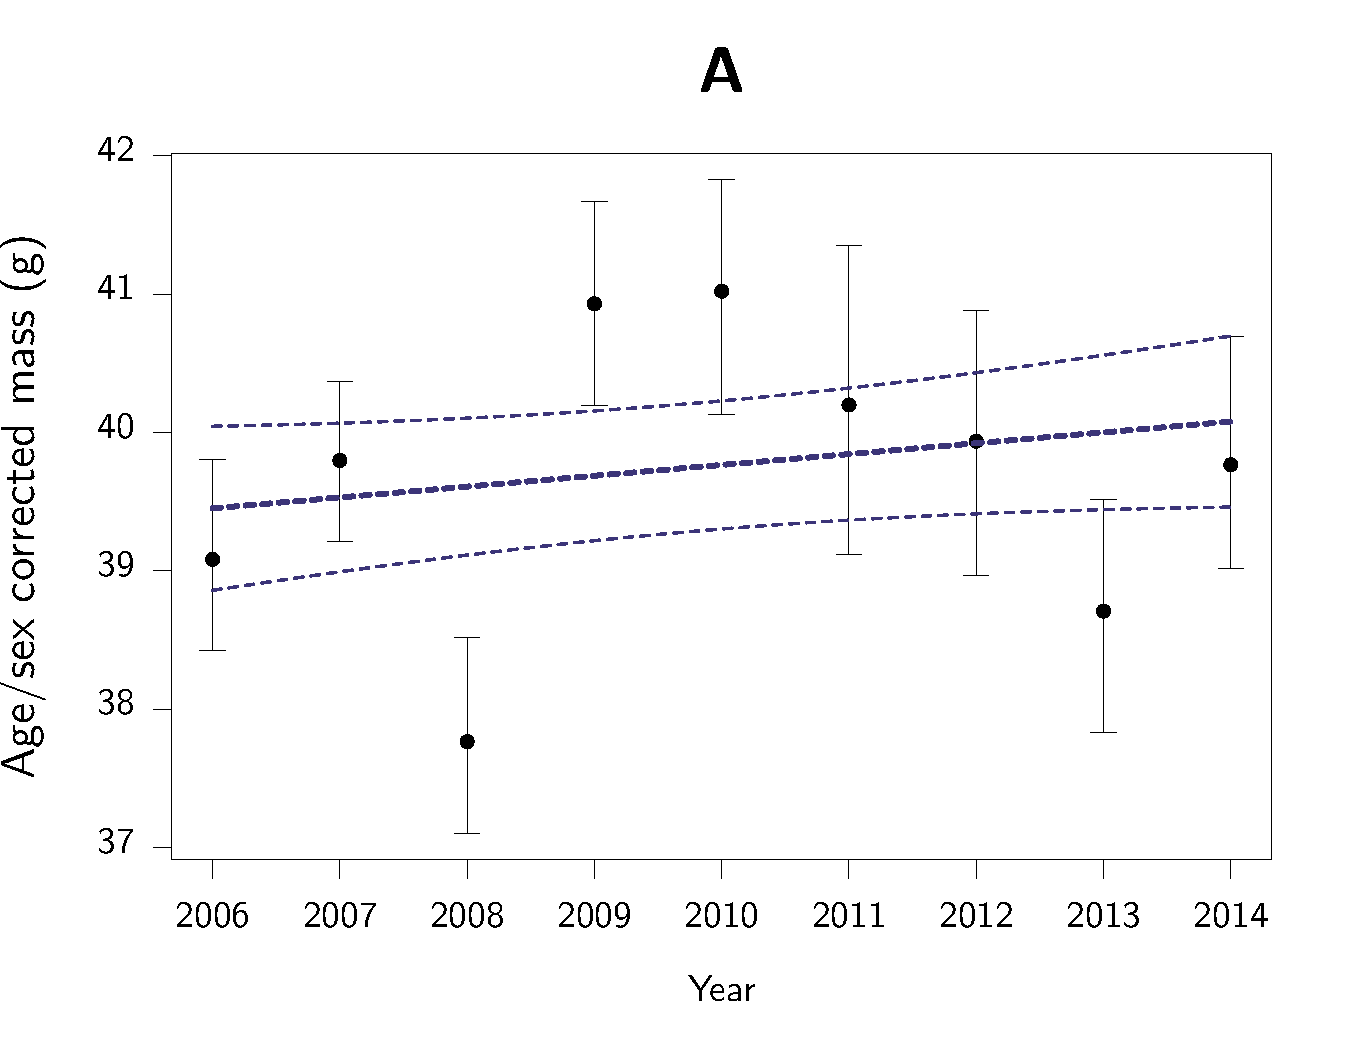
\includegraphics[width=0.49\textwidth]{FiguresStasis/PhenoTrends-1}
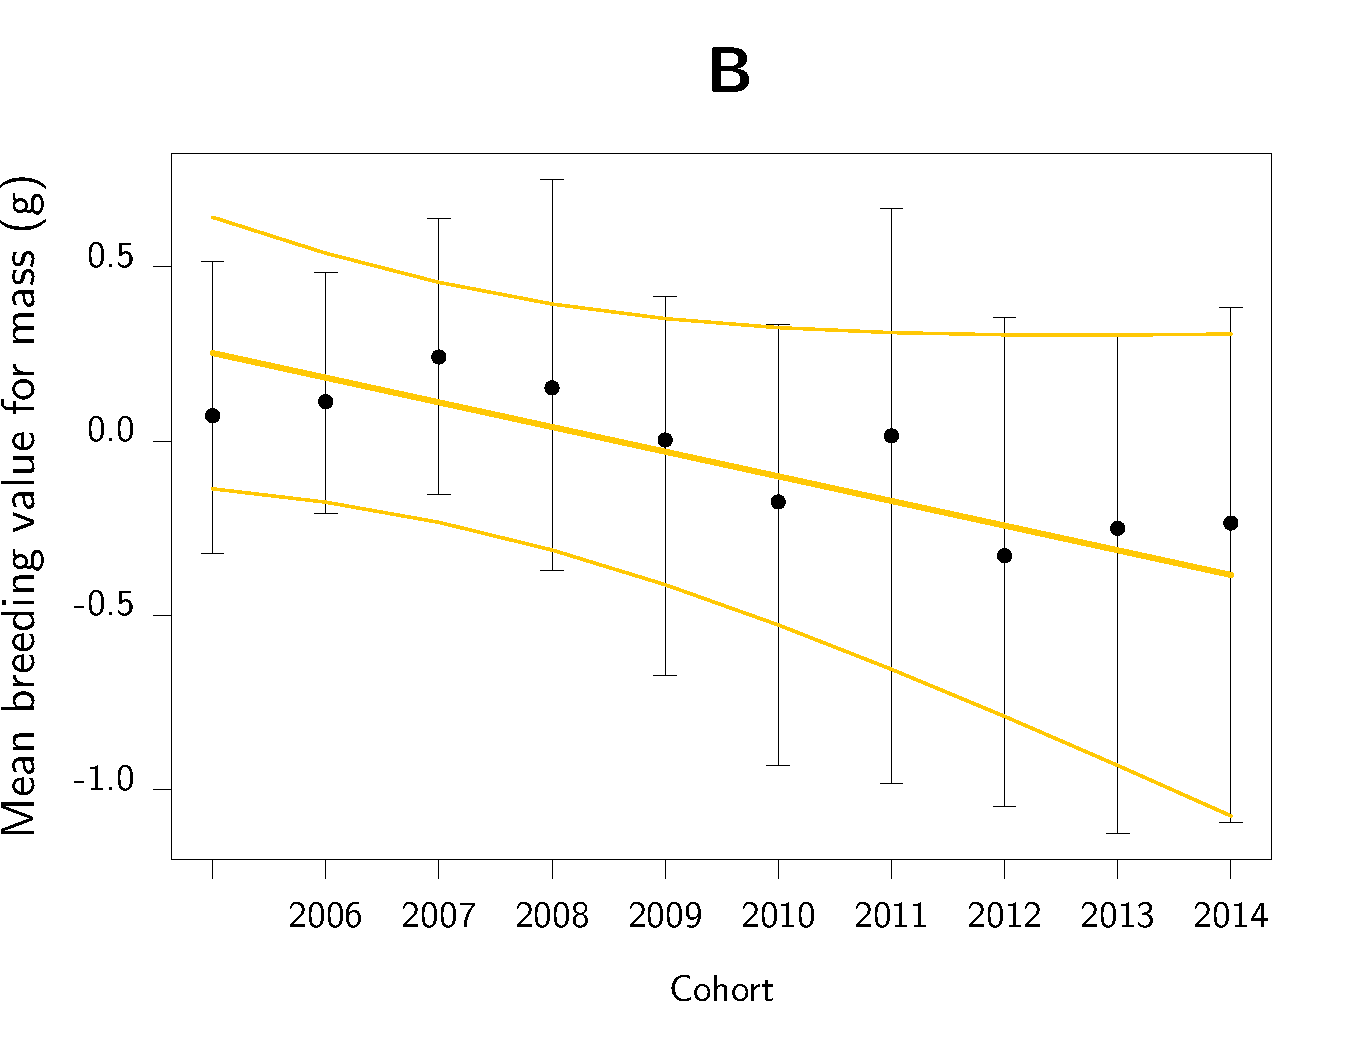
\includegraphics[width=0.49\textwidth]{FiguresStasis/BlupsTrendMass-1}
\end{center}
\caption{\footnotesize\textbf{Temporal variation in mass and estimated breeding values for mass.} (\textbf{A}): Year-specific mean mass corrected for age, sex and date of measurement, with 95\%CI. (\textbf{B}): Cohort-specific mean estimated breeding value for mass with their 95\%CI and the trend in breeding value with 95\%CI. Note the different of scale on the y-axes.}
\label{fig:trends}
\end{figure}


Given these estimates of selection ($S$) and heritability ($h^2$), the breeder's equation ($R=h^2S$) predicts an adaptive evolutionary response ($R$) in body mass \parencite{Lynch1998,Morrissey2012sts}, i.e. an increase in the mean breeding value for body mass over time, of 0.17 g/year (95\%CI [0.07;0.28]; Fig. \ref{fig:gch}A UBE).  However, after correcting for changes in demographic structure (i.e. accounting for sex and age effects, see Fig. \ref{fig:pop}), over the past nine years (approximately eight generations), the change in mean body mass is not significant and small at best (0.08 g/y; 95\%CI [-0.02;0.18]; p=0.14). This apparent mismatch between the predicted evolutionary change based on the breeder's equation and the phenotypic change observed provides yet another example of the stasis paradox \parencite{Merila2001}.

To test whether the predicted positive genetic trend, i.e. an increase in breeding values, is being masked by an opposing phenotypically plastic response \parencite{Merila2001,Hadfield2011}, we directly estimated the additive genetic covariance between mass and fitness. Based on the Robertson-Price's equation, this provides an unbiased estimate of the rate of genetic change per generation \parencite{Robertson1966,Price1970,Morrissey2012sts}. Contrary to our prediction, this estimate of genetic change in mass is strongly negative and highly significant ($p_\mathrm{MCMC}<0.001$; Fig. \ref{fig:gch}A GCPE). When normalized by a mean generation time of 1.2 years, this provides a rate of evolutionary change of -0.29 g/year (95\%CI [-0.55; -0.07]) or approximately 8,600 Darwins, which is in line with other rates of ``micro-evolution'' (e.g. between 3,700 and 45,000 Darwins in the Trinidadian guppies \parencite{Reznick1997}). Importantly, this rate of evolution is unlikely to have happened solely through genetic drift ($p_\mathrm{MCMC}<0.001$; Fig. \ref{fig:drift} and \ref{fig:driftcomp}) \parencite{Hadfield2010b}, and therefore most likely reflects a response to selection favouring genetically lighter individuals. 

\begin{figure}[ht]
{\centering
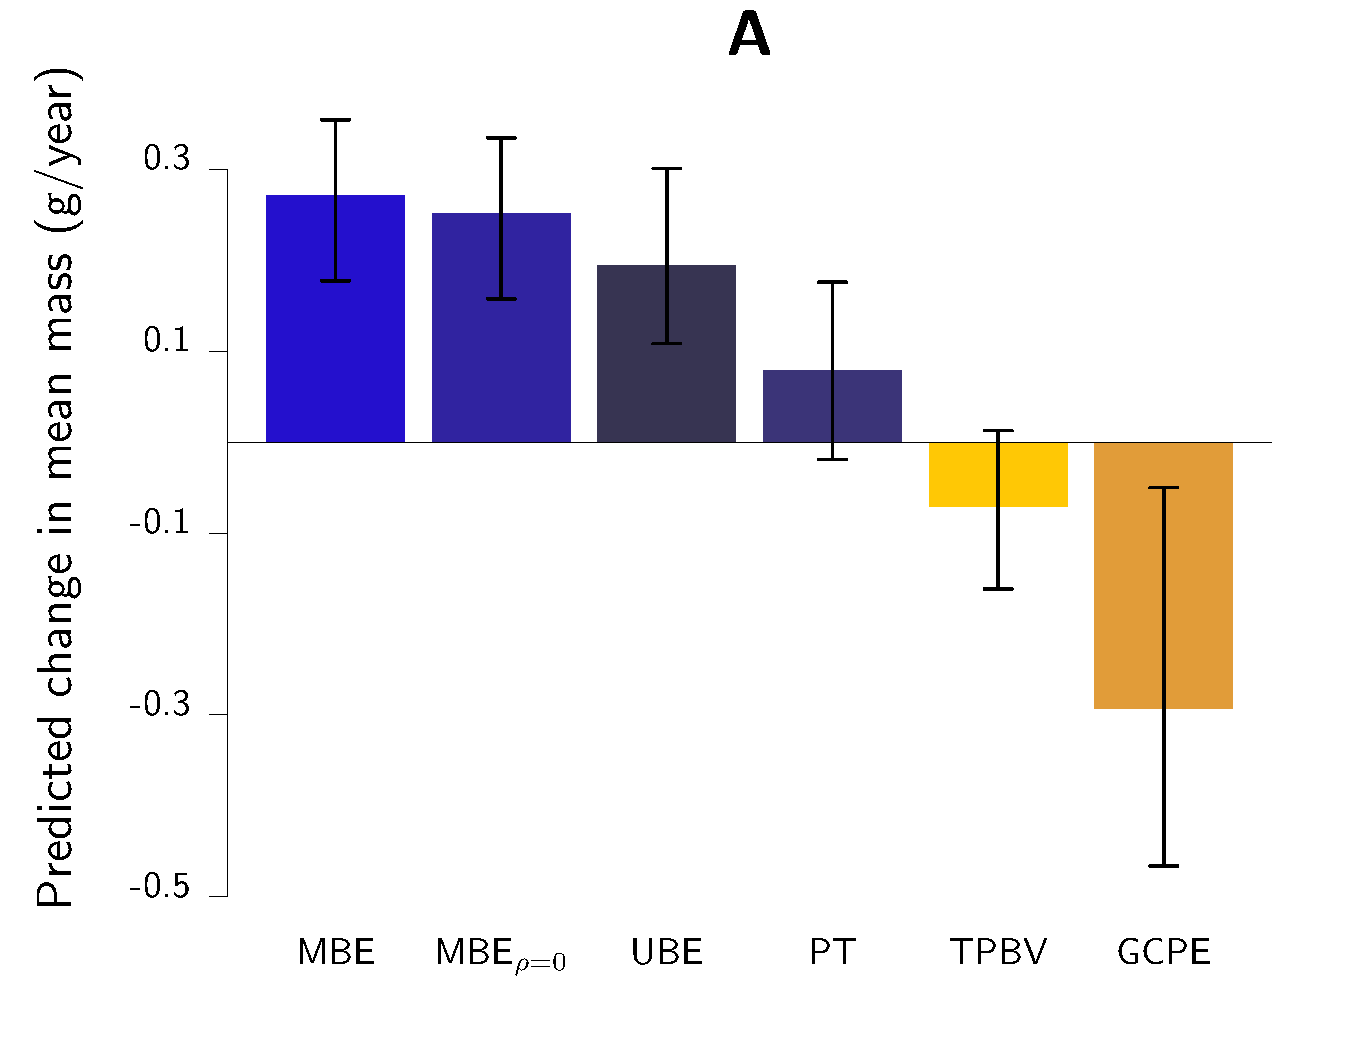
\includegraphics[width=0.49\textwidth]{FiguresStasis/AllChangeMass-1}
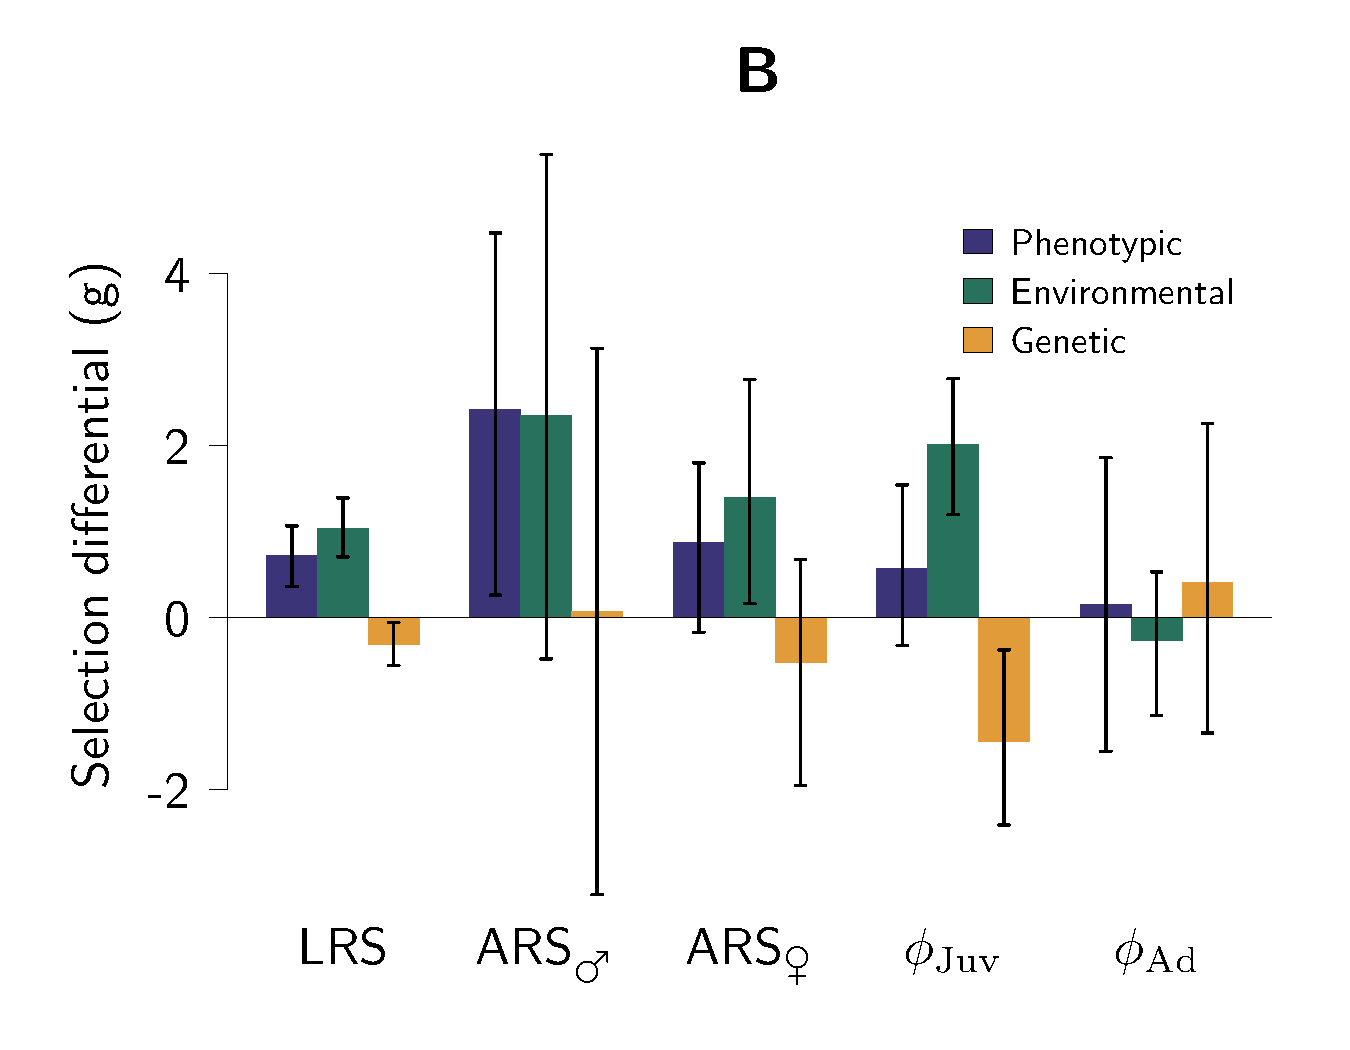
\includegraphics[width=0.49\textwidth]{FiguresStasis/SelectionS-1}
}
\caption{\footnotesize \textbf{Predicted and observed rates of evolutionary change.} (\textbf{A}): Rates of evolutionary change predicted by (from left to right) the breeder's equation in its multivariate form (MBE), the multivariate breeder's equation while constraining the genetic correlations to zero (MBE$_{\rho=0}$), and the univariate breeder's equation (UBE), followed by the phenotypic trend (PT), the trend in predicted breeding values (TPBV) and the genetic change estimated by the Price equation (GCPE). (\textbf{B}): Phenotypic, genetic and environmental selection differential for total selection (LRS), fertility selection in males (ARS$_{\male}$) and females (ARS$_{\female}$), viability selection in juveniles ($\phi_\mathrm{Juv}$) and in adults ($\phi_\mathrm{A}$). Both panels show posterior modes, with vertical lines indicating 95\%CI.}
\label{fig:gch}
\end{figure}

This result was confirmed by an independent estimate using best linear unbiased predictors (BLUPs) of breeding values for mass: Taking into account the non-independence of BLUPs and sampling variance \parencite{Postma2006,Hadfield2010b}, we find that predicted breeding values have declined over the past nine years (-0.07 g/year, $p_\mathrm{MCMC}$=0.06; Fig. \ref{fig:trends}B \& Fig. \ref{fig:gch}A TPBV), and this despite the BLUPs approach being potentially biased towards the phenotypic trend \parencite{Postma2006} (i.e. in this case toward zero). This negative trend, combined with the fact that the phenotypic mean has either remained constant or has shown a slight increase (see above), implies that the plastic component of body mass must have increased. Although the cause of this increase remains unknown, population size has declined over the study period (Fig. \ref{fig:pop}), which may have resulted in an increase in the per-capita resource availability (i.e. density dependence). Alternatively, the absolute food availability or quality may have improved. Interestingly, although these environmental changes may be coincidental, they may also be a direct result of a change in the selection regime or the evolutionary change toward smaller size \parencite{Cooke1990, Hadfield2011}.

As the phenotypic selection differential ($\sigma_{P(m,\omega)}$) is equal to the sum of the additive genetic and environmental covariances between mass and rLRS ($\sigma_{A(m,\omega)}$ and $\sigma_{E(m,\omega)}$, respectively) \parencite{Robertson1966,Price1970,Morrissey2012sts}, it follows that because $\sigma_{P(m,\omega)}$ is positive and $\sigma_{A(m,\omega)}$ is negative, the environmental covariance must be large and positive (Fig. \ref{fig:gch}B LRS). In other words, while environmental conditions that make voles heavy (for instance abundance of food or lack of parasites) also make them successful at reproducing and surviving, there is no causal \emph{positive} relationship between breeding values for mass and fitness (Fig. \ref{fig:HypA}). It is this difference in sign between $\sigma_{A(m,\omega)}$ and $\sigma_{E(m,\omega)}$ which represents an extreme violation of the breeder's equation (which assumes ${\sigma_{A(m,\omega)}}/({\sigma_{A(m,\omega)}+\sigma_{E(m,\omega)}})=h^2$). Hence, our initial prediction of evolution was wrong, demonstrating that phenotypic estimates of selection may provide severely biased predictions of the evolutionary trajectories of wild populations. But \emph{why} is evolution taking place in a direction that is opposite to apparent phenotypic selection?

\begin{figure}[h]
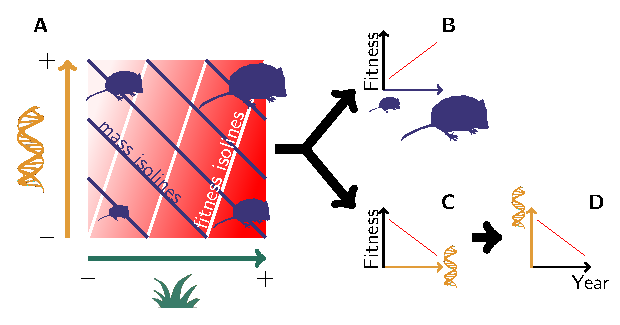
\includegraphics[width=0.9\textwidth]{FiguresStasis/Fig3}
\caption{\footnotesize \textbf{Schematic representation of why adaptive evolution goes opposite to apparent selection.} 
(\textbf{A}) Both genetic variation (orange) and environmental variation (green) contribute to phenotypic variation in mass (purple) in an additive and equivalent way: large voles are the result of genes for being large and of a favourable environment. Therefore, mass isolines form an angle of $45^\circ$ with both axes. However, the effect the fitness effect of the environmental component of mass variation is not the same as the fitness effect of the genetic component of mass variation: Fitness increases (the redder the fitter) with increasing environmental effects on mass, but decreases with increasing genetic effects on mass, as illustrated by fitness isolines (white). This pattern leads to (\textbf{B}) a phenotypic selection for heavier voles, along with (\textbf{C}) a ``genetic selection'' for lighter genotypes, thus leading to (\textbf{D}) an evolution towards lighter voles. Panel (\textbf{A}) should not be mistaken for a genotype-by-environment interaction: genetic and environmental effects are additive both for mass and for fitness. The additive effects on mass do not map on the additive effects on fitness, however.}
\label{fig:HypA}
\end{figure}

Indirect selection may be acting on body mass through one or more traits with negative genetic correlations with mass \parencite{Lande1983,Morrissey2012constraints}. However, the genetic correlations among the three morphological traits for which we have data\textemdash body mass ($m$), body length ($b$) and tail length ($t$)\textemdash are all positive (estimates and 95\%CI: $\rho_{m,b}=0.79$ $[0.06;0.93]$; $\rho_{m,t}=0.40$ $[0.01;0.66]$; $\rho_{t,b}=0.56$ $[-0.04;0.85]$), and the predicted response based on the multivariate breeder's equation (Fig. \ref{fig:gch}A MBE) is very similar to that based on its univariate counterpart (Fig. \ref{fig:gch}A UBE), as well as to that based on a multivariate breeder's equation constraining the correlations to zero (Fig. \ref{fig:gch}A MBE$_{\rho=0}$). Furthermore, for parent-offspring conflict between size and fertility to constrain the evolution of size, the genetic correlation between juvenile size and adult annual reproductive success should be negative \parencite{Rollinson2015b}. In our study population this correlation was 0.21, 95\%CI $[-0.24;0.74]$), arguing against a role for a trade-off between fertility and offspring size in driving the observed evolution toward smaller sizes. Although we cannot exclude that selection on other, unmeasured, traits does indirectly shape body mass evolution,  genetically correlated traits are not more likely to constrain than to facilitate adaptation \parencite{Agrawal2009}. This suggests that the counter-intuitive direction of evolution is really due to selective pressures acting on mass, but given that selection acts on phenotypes rather than genotypes, which aspect of an individual's body mass is the subject of negative selection? 

To identify the fitness component that is negatively associated with genes for being heavy, we computed sex- and age-specific genetic covariances between mass and fitness components. Whereas the genetic covariances between mass and both relative annual reproductive success and adult survival are close to zero in both sexes (Fig. \ref{fig:gch}B), the genetic covariance between mass and over-winter survival is negative in juveniles (-0.98 [-2.44;-0.18] on a logit scale, $p_\mathrm{MCMC}$=0.01). Because the genetic correlation between juvenile and adult mass is positive ($r_A=0.88$; 95\%CI [0.39;1]) and significantly different from 0 (p=0.004) but not 1 (p=0.35), selection on juvenile mass can shape genetic variance for mass at all ages, and thereby contribute to the observed negative genetic change \parencite{Chevin2015a}. While this shows that negative viability selection of juvenile mass is responsible for the genetic change toward smaller individuals, how come survival is higher for heavier phenotypes \emph{and} lighter genotypes? 

Juvenile mass covaries positively with both within- and between-year survival ($p=0.009$ and $p=1.3\times10^{-6}$, respectively). However, juveniles can only be captured when they first leave their burrow, at an age of approximately three weeks \parencite{Janeau1997} and a weight of 12 to 20 g, and they may continue to be captured until the end of the season, when they can reach weights of up to 50 g. Because of growth, mass measurements are therefore not directly comparable among juveniles. Indeed, at least part of the positive estimated selection on juvenile mass is likely to be mediated by the simultaneous increase, with age, of mass and of the probability of survival to the next year \parencite{Hadfield2008}. In addition, viability selection introduces non-random missing data, which results in biased estimates of viability selection on mass \parencite{Hadfield2008,Steinsland2014}. This led us to hypothesise that the positive phenotypic association between juvenile body mass and survival was largely the result of ontogeny non-random missing data, whereas the negative genetic association is driven by selection imposed by the necessity to have completed growth before the end of the growing season. 


The (co)variance decompositions presented above have the advantage that they do not make causative statements. For example, a genetic covariance describing the rate of evolution has a self-contained, tautological, meaning and does not make any assumptions with respect to its causes \parencite{Frank2012IV}. However, if we are to identify the target of juvenile viability selection, we must adopt a more traditional hypothesis testing framework. Although, as we emphasised above, inferring a causal relationship between a trait and fitness based on their covariance requires great care, we set out to test the hypothesis that when the period favourable for growth is limited, selection favours lighter juveniles, as they require less time to reach their adult size. 

To obtain an estimate of viability selection that is unbiased by growth and non-random missing data due to mass-dependent mortality occurring after the first capture \parencite{Hadfield2008}, we used a Bayesian model to simultaneously infer birth dates and growth curves for all juveniles observed at least once, irrespective of when and how often they have been captured. Although we cannot account for viability selection acting before the first capture, this model enabled us to quantify viability selection on age-corrected juvenile mass\textemdash i.e. asymptotic or predicted adult mass\textemdash, and thereby compare all individuals at the same developmental stage, irrespective of their fate. 

Inferred birth dates revealed that snow fallen during the preceding winter is a major ecological factor constraining the onset of reproduction in spring, with reproduction starting on average 40 days after the snow has melted (SE 4.5, $p=4\times 10^{-5}$) (Fig. \ref{fig:ResA}A). As a consequence, juveniles only have a limited amount of time to grow and reach their adult mass before the return of winter. As growth rate and predicted adult mass are slightly negatively correlated (correlation -0.077; 95\%CI [-0.150; -0.002]), juveniles with a smaller adult mass on average require less time to complete development. If individuals that have not completed development before the arrival of winter pay a survival cost, for example due to trade-offs between growth and vital physiological processes \parencite{Stearns1986,Owens1999}, this generates selection for small size, especially for juveniles born toward the end of the season (Fig. \ref{fig:ResA}D and Fig. \ref{fig:scheme}). 

To test this, we quantified the strength of survival selection acting on predicted adult mass, which was slightly negative when averaged over all years and the complete reproductive season ($p_\mathrm{MCMC}$=0.13), but interacted strongly and significantly with the number of days between birth and the first snowfall of that year ($p_\mathrm{MCMC}$=0.008). This implies that individuals born closer to the first snowfall are more strongly selected for a low adult mass, and that the length of the snow-free period in a given year determines the total selection experienced by the population in that year. Interestingly, at our field site, the length of the snow-free period in the years 2008 to 2014 has been significantly shorter than during the preceding six years (Fig. \ref{fig:ResA}B). The latter coincides with a period of exceptionally high snowfall, low temperatures and a long duration of snow cover, across the Swiss Alps \parencite{Beniston2012}.

Our model estimates that in 2006 and 2007, when the snow-free period was long (Fig. \ref{fig:ResA}B), most juveniles reached their adult mass before the first snowfall, and there was hence no selection on asymptotic mass ($\beta=-0.002$, SE= 0.0006, $p_\mathrm{MCMC}$=0.47, Fig. \ref{fig:ResA}C; D; \ref{fig:driftcomp}). However, in all subsequent years, the snow-free period was much shorter, and there was selection for a lower asymptotic mass ($\beta=-0.10$, SE=0.0008, $p_\mathrm{MCMC}$=0.009). This suggests that the shortening of the snow-free season, and thereby selection for lower asymptotic mass, is a novel phenomenon that the population is currently in the process of adapting to. Although model complexity and data availability prohibit disentangling genetic and environmental sources of variation in asymptotic mass among individuals and over time, and we cannot rule out the possibility that the selective pressure we identified is not causative \parencite{Morrissey2014}, the cohort born in 2013 had an estimated adult mass that was 1.02 g smaller than the cohort born in 2006 (p=0.05). This shrinkage is predicted to have increased population-level juvenile survival by 2.5\%, and to have contributed positively to population recovery (Fig. \ref{fig:pop}). 

\begin{figure}[h]
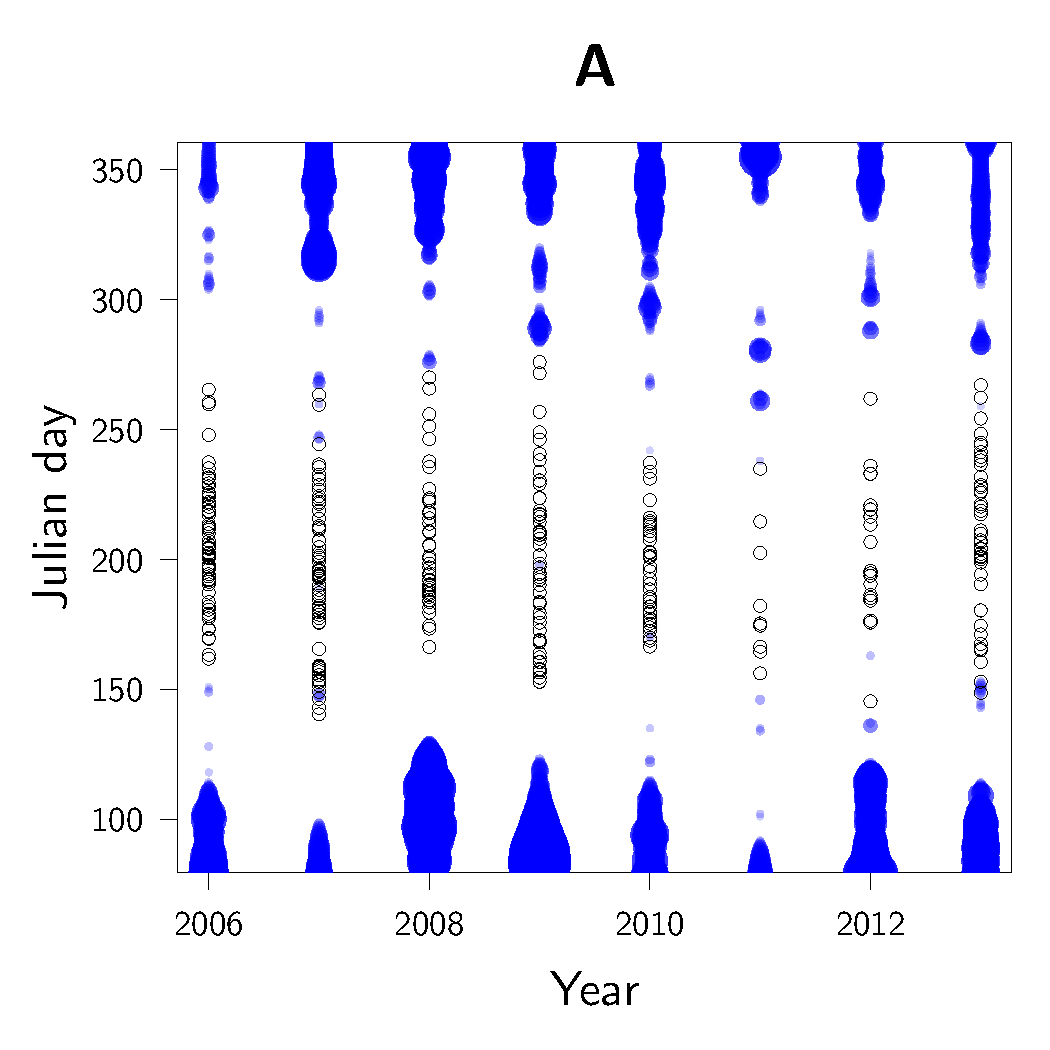
\includegraphics[width=0.5\textwidth]{FiguresStasis/BDsnow-1}
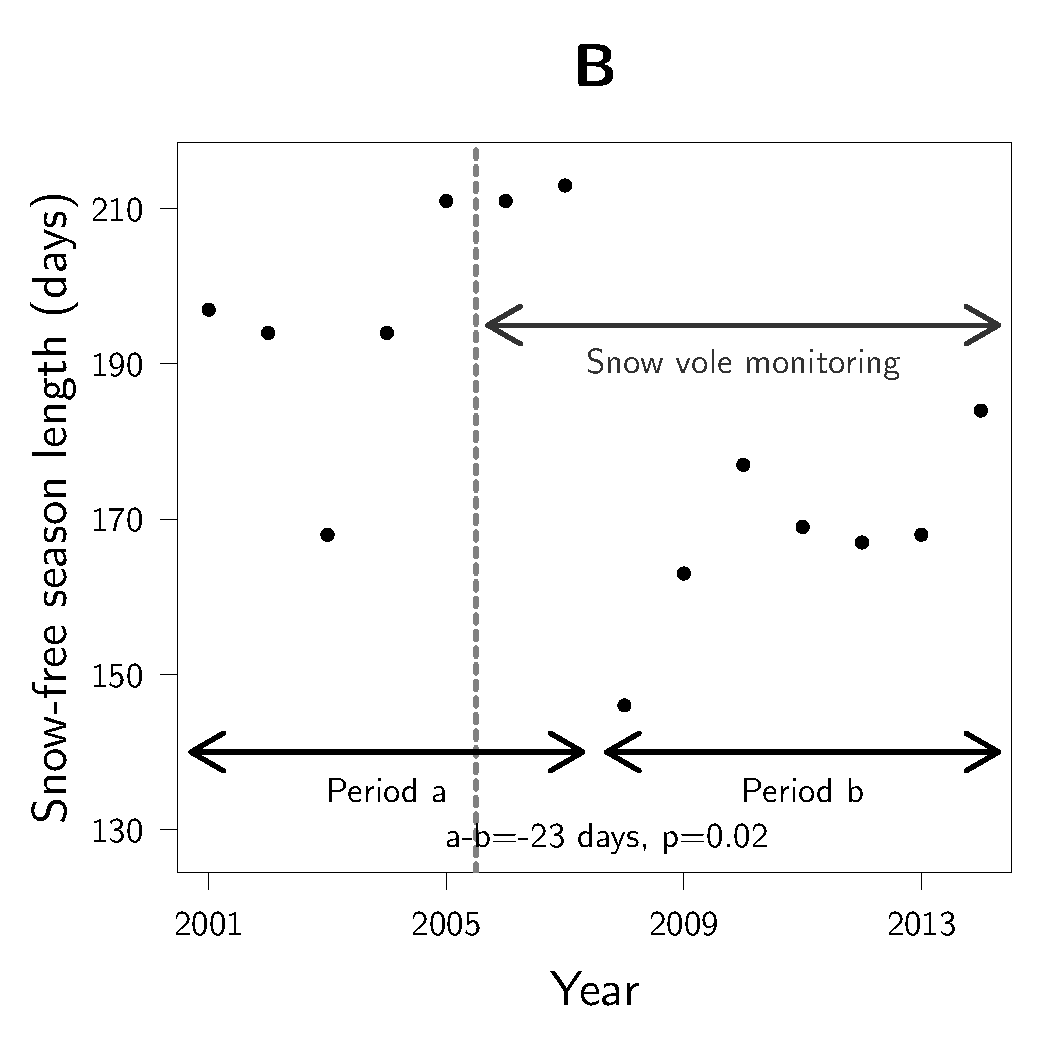
\includegraphics[width=0.5\textwidth]{FiguresStasis/Climatic_trend-1}
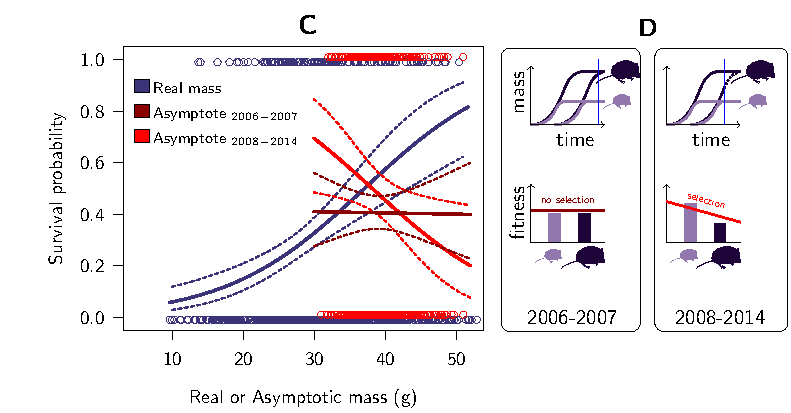
\includegraphics[width=1\textwidth]{FiguresStasis/Fig3b}
\caption{\footnotesize \textbf{Snow-free season, timing of reproduction and selection for asymptotic mass.} (\textbf{A}): Births (black dots) only occur during the snow free season (snow depth in blue), (\textbf{B}): which in 2008-2014 has been shorter than in the preceding 8 year. Therefore, (\textbf{C}) despite a positive phenotypic selection on body mass (blue), asymptotic mass was selectively neutral in 2006-2007 (brown), and was negatively selected in 2008-2014 (red), as a result of (\textbf{D}) the selective disappearance of heavy individuals that were born too close to the onset of winter (blue vertical line) during 2008-2014.}
\label{fig:ResA}
\end{figure}

\section{Conclusion}
We have exploited a case of apparent evolutionary stasis to gain a deeper insight into the evolutionary dynamics of natural populations, and the selective pressures that shape them. Whereas estimates of selection and evolution based on phenotypic data alone can easily mislead our understanding of the selective and evolutionary processes in natural populations, a quantitative genetic framework applied to individual-based long-term data allows us to unravel evolutionary and environmental changes over time, and to obtain unbiased estimates of selection. This has resolved a case of apparent evolutionary stasis, and provided a comprehensive empirical demonstration of contemporary adaptive evolution in response to a climatic fluctuation. 

\section{Methods}
\paragraph{Snow vole monitoring.}
Monitoring of the snow vole population began in 2006 and the present work uses data collected until the fall of 2014. The snow vole monitoring was authorised by the \textit{Amt f\"{u}r Lebensmittelsicherheit und Tiergesundheit}, Chur, Switzerland. The study site is located at around 2030m above sea level, in the central eastern Alps near Churwalden, Switzerland ($46^{\circ}$48' N, $9^{\circ}$34' E). It consists of scree, interspersed with patches of alpine meadows and surrounded by habitat unsuitable for snow voles: a spruce forest to the West, a cliff to the East and large meadows to the North and South. In accordance with it being considered a rock-dwelling specialist \parencite{Janeau1997}, at our study site it is almost never captured outside of the rocky area. Given that it is ecologically fairly isolated, we are able to monitor the whole population.
Trapping throughout the whole study area takes place during the snow-free period, between late May and mid-October. One trapping session consists of four trapping nights. Analyses presented here are based on a total of two (in one year), three (in three years) or five (in five years) trapping sessions per season.
All newly-captured individuals weighing more than 14 g are marked with a subcutaneous passive transponder (PIT, ISO transponder, Tierchip Dasmann, Tecklenburg). Additionally, an ear tissue sample is taken (maximum 2 mm in diameter) using a thumb type punch (Harvard Apparatus) and stored in 100\% ethanol at $-20^{\circ}\mathrm{C}$. DNA extracted from these samples is genotyped for 18 autosomal microsatellites developed for this population \parencite{Wandeler2008}, as well as for the \textit{Sry} locus to confirm the sex of all individuals. Finally, another Y-linked marker as well as a mitochondrial marker is used check for errors in the inferred pedigree (see below). An identity analysis in \verb+CERVUS+ v.3.0 \parencite{Marshall1998} allows us to identify animals sampled multiply, either because they lost their PIT, or because at their first capture as a juvenile they were too small to receive a PIT.
All the analyses were carried out in \verb+R+ \parencite{R2014}. Specific packages are referenced below.

\paragraph{Pedigree inference.}
Parentage was inferred by simultaneously reconstructing paternity, maternity and sibship using a maximum likelihood model in \verb+MasterBayes+ \parencite{Hadfield2006}. Parentage was assigned using a parental pool of all adults present in the examined year and the previous year, assuming polygamy and a uniform genotyping error rate of 0.5\% for all 18 loci. As it is known that in rare cases females reach sexual maturity in their year of birth \parencite{Janeau1997}, we matched the genotypes of all individuals against the genotypes that can be produced by all possible pairs of males and females. We retrieved the combinations having two or less mismatches (out of 18 loci) and ensured that parental links were not circular and were temporally consistent. This way, we identified eight young females as mothers of animals born in the same year, with a known father but a mother not yet identified. All of these females were relatively heavy ($>$33 g) at the end of the season and their home-ranges matched those of their putative offspring.
Finally, the pedigree was checked using a polymorphic Y-linked locus developed for this population \parencite{Wandeler2011}, as well as a fragment of the mitochondrial DNA control region, amplified using vole specific primers \parencite{Haring2000}. There were no inconsistencies between the transmission of these three markers and the reconstructed pedigree.
The final pedigree had a maximum depth of 11 generations and a mean of 3.8 generations. It consisted of 987 individuals with 458 full-sibling pairs, 3010 half-sibling pairs, 764 known maternities and 776 known paternities, so that, excluding the base population, 86\% of the total parental links were recovered.

\paragraph{Traits.}
The recapture probability from one trapping session to the next was estimated to be 0.924 (SE 0.012) for adults and 0.814 (SE 0.030) for juveniles using mark-recapture models. Thus, with three trapping session a year, the probability not to trap an individual present in a given year is below $10^{-3}$. Not surprisingly, no animal was captured in year $y$, not captured in $y+1$, but captured or found to be a parent of a juvenile in $y+2$ or later. Therefore, capture data almost perfectly matches over-winter survival. However, as is almost always the case in these type of studies, we are unable to separate death from permanent emigration. Importantly however, as both have the same consequences on the population level, this does not affect our evolutionary predictions.

Annual and lifetime reproductive success (ARS and LRS, respectively) were defined as the number of offspring attributed to an individual in the pedigree, either over a specific year or over its lifetime. 56 individuals born of local parents were not captured in their first year, but only as adult during the next summer, probably because they were born late in the season and we had only few opportunities to catch them. This means that we miss a fraction of the juveniles that are not observed in their first year and die, or emigrate, during the following winter. We acknowledge that this means that our measures of ARS and LRS partly conflate adult reproductive success and the viability of those juveniles that were never observed, but our measures are the most complete measures of reproductive success available in this system.

We used relative LRS ($\omega$) as proxy for fitness \parencite{Lande1983}, where $ \omega_{i} = \frac{\mathrm{LRS}_{i}}{\frac{1}{N_{s,t}}\sum_{j=1}^{N_{s,t}} {\mathrm{LRS}_{j,t}}} $. Here, $N_{s,t}$ is the number of individuals of same sex as the focal individual $i$, present in the cohort $t$, so that $\frac{1}{N_{s,t}}\sum_{j=1}^{N_{s,t}} {\mathrm{LRS}_{j,t}}$ is the sex-specific, cohort-specific mean of LRS. The latter is required as the mean LRS differs between males and females due to imperfect sampling \parencite{Morrissey2012sts}. In addition, we used cohort-specific means in order to account for variations in population size.

Generation time was defined as the mean age of parents at birth of their offspring\parencite{Charleworth1994}.

Mass ($m$) was measured to the nearest gram with a spring scale. Both body length ($b$), measured from the tip of the nose to the base of the tail, and tail length, measured from the tip to the base of the tail ($c$), were measured to the closest mm with a calliper while holding the animal by the tail. 

\paragraph{Selection.}
Selection differentials were estimated using bivariate linear mixed models, as the individual-level covariance between fitness and mass (corrected for sex, age and cohort). However, while this provides the best estimate of the within-generation change in trait mean due to selection \parencite{Lande1983}, because the distribution of fitness is not Gaussian, it cannot be used to estimate confidence intervals. Hence, the statistical significance of selection was tested using a univariate over-dispersed Poisson generalized linear mixed model (GLMM) in which LRS was modelled as a function of individual standardized mass and including sex and age as covariates and cohort as a random effect. Note that the latter estimates the effect of mass on a transformed scale, and therefore cannot be directly used to quantify an effect of selection on the original scale measured in grams \parencite{Mitchell-Olds1987}. The significance based on the basis of the GLMM was confirmed by non-parametric bootstrapping. Similarly, we tested for the significance of selection through ARS only, using an over-dispersed Poisson GLMM including sex as a fixed effect, and year and individual as random effects. 

The estimation of survival selection is facilitated by the fact that the year-to-year individual recapture probability is effectively 1. Therefore, selection on year-to-year survival was tested for by a binomial GLMM. This model included sex, age and their interaction as fixed effects, and year as a random effect.

In order to integrate the uncertainty in the estimation of selection with the uncertainty in the estimation of heritability when predicting the rate of evolution, selection differentials and gradients were also obtained from the multivariate animal model presented below.

\paragraph{Quantitative genetic analyses.}
We used uni- and multivariate animal models to estimate additive genetic variances, covariances and breeding values \parencite{henderson1984,Lynch1998,Kruuk2004} with \verb+MCMCglmm+ \parencite{Hadfield2010a}. All estimations were carried out in a Bayesian framework in order to propagate uncertainty when computing composite statistics such as heritabilities and rates of genetic change \parencite{Stinchcombe2014}. All estimates provided in the text are posterior modes and credibility intervals are highest probability density intervals at the 95\% level.
All the animal models were run for 1,300,000 iterations with a burnin of 300,000 and a thinning of 1,000, so that the autocorrelations of each parameter chain was less than $0.1$. Convergence was checked graphically and by running each model twice.

\paragraph{Univariate models: }
We first carried out univariate model selection, fitting models without an additive genetic effect, to determine which fixed and random effects to include. Based on AICc \parencite{Burnham2002c}, and fitting the models by Maximum of Likelihood in \verb+lme4+ \parencite{Bates2014a}, we obtained a model that predicts the mass $m_{i,t}$ of individual $i$ at time $t$ by: age, as a factor (juvenile or adult); sex as a factor; the interaction between age and sex; Julian dates and squared Julian dates, which were centered and divided by their standard deviations in order to facilitate convergence; the interaction between age and Julian date; the interaction between sex and Julian date; the three way interaction between age, sex and Julian dates; a random intercept for individual; and a random intercept for year. The inclusion of year accounts for non-independence of observation within years, while individual accounted for the non-independence of repeated measurements made on the same individual \parencite{Kruuk2007}. 
We then fitted an animal model by adding a random intercept modelling variance associated with mother identity \parencite{Kruuk2004}, and a random intercept modelling additive genetic variance. Although it was not included in the best models, we kept inbreeding coefficient (estimated from the pedigree) as a covariate, because leaving it out could bias the later estimation of additive genetic variation \parencite{deBoer1993}. Nevertheless, animal models fitted without this covariate gave indistinguishable estimates.

\paragraph{Multivariate models: }
Univariate animal models can be expanded to multivariate models in order to estimate genetic correlations, genetic gradients and genetic differentials.

\begin{align*}
[\boldsymbol{m},
\boldsymbol{l},
\boldsymbol{t},
\boldsymbol{\omega}]
\sim
\boldsymbol{bX}+\boldsymbol{D_1a}+\boldsymbol{D_2m}+\boldsymbol{D_3p}+\boldsymbol{D_4y}+\boldsymbol{Ir.}\\
\end{align*}
Here $\boldsymbol{X}$, $\boldsymbol{D_1}$, $\boldsymbol{D_2}$, $\boldsymbol{D_3}$ and $\boldsymbol{D_4}$ are design matrices relating observations to the parameters to estimate, $\boldsymbol{b}$ is a matrix of fixed effects, $\boldsymbol{a}$, $\boldsymbol{m}$, $\boldsymbol{p}$ and $\boldsymbol{y}$ are random effects accounting for the variance associated with breeding value, mother, permanent environment and year, respectively. The fixed part of the model matches that used for each trait in univariate models.

The most important aspect of this model is that $\boldsymbol{a}$, the matrix of breeding values, follows a multivariate normal distribution:
\begin{equation}\boldsymbol{a}
\sim MVN\left(\boldsymbol{0},
\boldsymbol{A \otimes G}
\right)
\end{equation}
where $\boldsymbol{A}$ is the relatedness matrix describing the relatedness among all individuals, and $\boldsymbol{G}$ is the G-matrix, containing the additive genetic variances and covariances among all traits.\\

\begin{equation}
\boldsymbol{G}=\begin{pmatrix}
\sigma_{A}^2(m) & \sigma_{A}(m,l) & \sigma_{A}(m,t) & \sigma_{A}(m,\omega)\\
\sigma_{A}(m,l) & \sigma_{A}^2(l) & \sigma_{A}(l,t) & \sigma_{A}(l,\omega)\\
\sigma_{A}(m,t) & \sigma_{A}(l,t) & \sigma_{A}^2(t) & \sigma_{A}(t,\omega)\\
\sigma_{A}(m,\omega) & \sigma_{A}(l,\omega) & \sigma_{A}(t,\omega) & \sigma_{A}^2(\omega)\\
\end{pmatrix}.
\end{equation}

For any trait $z$, $\sigma_{A}(z,\omega)$ is the genetic differential, that is, the predicted rate of evolutionary change according to Robertson's secondary theorem of natural selection, or Price equation applied to genetic variation \parencite{Robertson1966, Price1970, Morrissey2012sts}. The Price equation is generally presented as a prediction of evolutionary change over the next generation, but it has also been used as a description of change \parencite{Heywood2005, Frank2012IV, Coulson2008}. We use this prediction retrospectively, as an estimation of the mean evolutionary change that has occurred during the study period, which makes the assumption that $\omega$ is a good measure of fitness, because when ``real fitness'' is used, the equation is a mathematical tautology, i.e. it is exact \parencite{Frank2012IV}. A deviation from this perfect fitness measure could come from random Mendelian segregation or systematic meiosis distortion. Our results were robust to the use of an annualized measure of fitness (annual reproductive success plus twice survival), and to standardizing fitness across all individuals, within years, within cohorts, and within sexes.

For two traits $z$ and $y$, the genetic correlation is $\frac{\sigma_{A}(z,y)}{\sigma_{A}(z)\sigma_{A}(y)}$.
The vector of selection differentials on the three traits ($\boldsymbol{S}$) was estimated as the sum of the vectors of covariances between traits and $\omega$ in the variance-covariance matrices for $\boldsymbol{a}$, $\boldsymbol{p}$ and $\boldsymbol{r}$; which was equivalent to the selection differential computed in the paragraph on selection above. We excluded the among-year level covariance from the selection differential, because (i) covariation between mass and fitness at the level of year does not correspond to selection as it does not occur among individuals (ii) due to the standardization of relative fitness at the level of cohorts, the among year variance and covariances involving $\omega$ were effectively zero ($\sigma_{Y}^2(\omega)<10^{-8}$). 
Let $\boldsymbol{G^\prime}$ be a subset of $\boldsymbol{G}$ excluding the column and the row that contain $\omega$.
The vector of selection gradients on the three traits ($\boldsymbol{\beta}$) was estimated as $\boldsymbol{(G^\prime+P^\prime+R^\prime)^{-1}S}$, where $\boldsymbol{P^\prime}$ and $\boldsymbol{R^\prime}$ are the equivalent of $\boldsymbol{G^\prime}$ for permanent environment effects and for residuals, respectively.

The prediction of the multivariate breeders equation is obtained by $\Delta \overline{\boldsymbol{Z'}}=\boldsymbol{G^\prime \beta}$, while the multivariate breeders equation ignoring genetic correlations is obtained by multiplying the $\boldsymbol{G^\prime}$ matrix by the identity matrix\parencite{Morrissey2012constraints}: $\Delta \overline{\boldsymbol{Z'}}=\boldsymbol{(G^\prime \times I)\beta}$.

To investigate the potential role of parent-offspring conflict, we estimated the genetic correlation between parental ARS and offspring mass using a bivariate animal model. For juvenile mass, we used predicted adult mass (i.e. age-corrected juvenile mass; see below). The model included sex, Julian dates and squared Julian dates as fixed effects for offspring mass, and only sex for ARS. 
\begin{align*}
[\boldsymbol{m_O},
\boldsymbol{ARS_P}]
\sim
\boldsymbol{bX}+\boldsymbol{D_1a}+\boldsymbol{D_2y}+\boldsymbol{Ir.}\\
\end{align*}

\paragraph{Test of genetic correlations: }
We used \verb+ASReml-R+ \parencite{Gilmour2014, Butler2009} to test the genetic correlation between mass in adults and in juveniles against 1 and 0, by considering them as two separate traits. We first ran an unconstrained model and then reran it with the genetic correlation parameter set to 0.99 (and not exactly to 1 because \verb+ASReml+ cannot invert matrices with perfect correlations), or 0 respectively. The fit of the unconstrained model was then compared to that of the two constrained models using a likelihood ratio test with one degree of freedom \parencite{Wilson2009}.

\paragraph{Birth date and growth prediction: }
Using the Bayesian programming environment \verb+JAGS+ \parencite{Plummer2003}, we fitted a multivariate Bayesian model to mass measurements of all 613 juveniles with mass data, and to their overwinter survival. The model simultaneously estimated individual growth curves\textemdash that is onset of growth (although this is referred to as ``birth date'' hereafter, this actually is the projected time when mass was zero, i.e. at conception), individual growth rates and asymptotic masses of all juveniles\textemdash and the effect of asymptotic mass on overwinter survival. The model clustered juveniles from the same mother born in the same year into litters (see e.g. \parencite{Cornulier2009} for a similar approach), assuming a maximum of five litters per year and assuming that successive litters are at least 20 days apart \parencite{Janeau1997}. Preliminary model selection, assuming no differences in asymptotic masses among individuals, selected a monomolecular growth model ($\Delta \mathrm{DIC} > 80$) over Gompertz and logistic models, as defined in \parencite{English2012}. The model accounted for measurement error in mass, assuming that the standard deviation of the errors was that observed in animals measured multiple times on the same day (2.05g).
In order to estimate the overall viability selection on asymptotic mass, we performed within the model a logistic regression of year-to-year survival on sex and asymptotic mass. In order to test for the effect of the length of snow free period on the selection on asymptotic mass, we reran the full model including time until the first snow fall and its interaction with asymptotic mass in the logistic regression. We use the estimates of these two models to predict the survival probability as a function of asymptotic mass for every year, or for groups of years, depending on the distribution of birth dates and on the timing of the first snow fall. 


Three MCMC chains were run for 6,300,000 iterations, with a burnin of 300,000 and a thinning of 6,000. Convergence was assessed by visual examination of the traces, and by checking that the $\hat{R}<1.01$. Convergence was not achieved for the litter affiliations of 25 individuals as well as for one asymptotic mass, thus generating a bit more uncertainty in the estimations. The fit of the model was assessed using posterior predictive checks on the predictions of individual masses (p=0.46) and survival probabilities (p=0.49).  
The \verb+JAGS+ code for this model can be found at \url{https://github.com/timotheenivalis/SelRepSel}.

\section*{Acknowledgements}
Thanks to Lauren Richardson, Tim Coulson, Alastair Wilson and two anonymous reviewers for constructive comments. Thanks to Wolf U. Blanckenhorn, Jarrod D. Hadfield, Lukas F. Keller, Marc K\'{e}ry, Hanna Kokko, Chelsea J. Little, Pirmin Nietlisbach, Barbara Tschirren and Ashley E. Latimer for comments and discussions on earlier versions of this work. Thanks also to the many field helpers. Weather data were provided by MeteoSwiss. The snow vole monitoring was authorised by the \textit{Amt f\"{u}r Lebensmittelsicherheit und Tiergesundheit}, Chur. Switzerland. T.B. is funded by a Swiss National Science Foundation project grant (\verb|31003A_141110|) awarded to EP. 

\printbibliography[heading=subbibliography]

\clearpage
\section{Supplementary information}

\begin{figure}[ht]
\centering
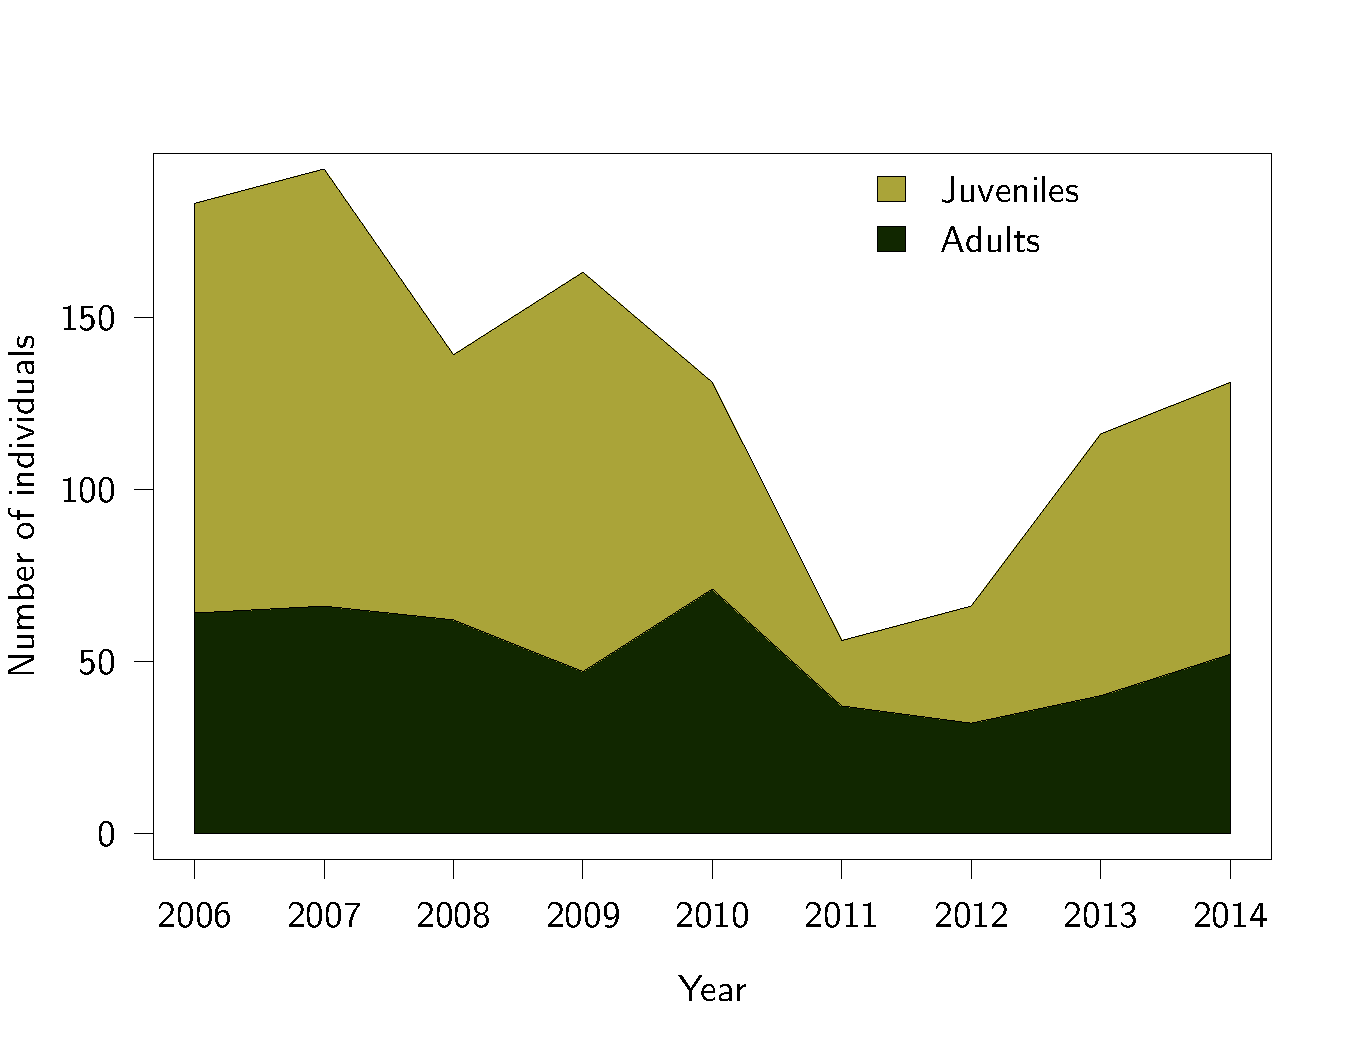
\includegraphics[width=0.5\textwidth]{FiguresStasis/PopulationTrend-1}
\caption{\footnotesize \textbf{Temporal variation in population size and age-structure.} Number of individual adults and of juveniles captured in each year.}
\label{fig:pop}
\end{figure}

\begin{figure}[h]
\centering
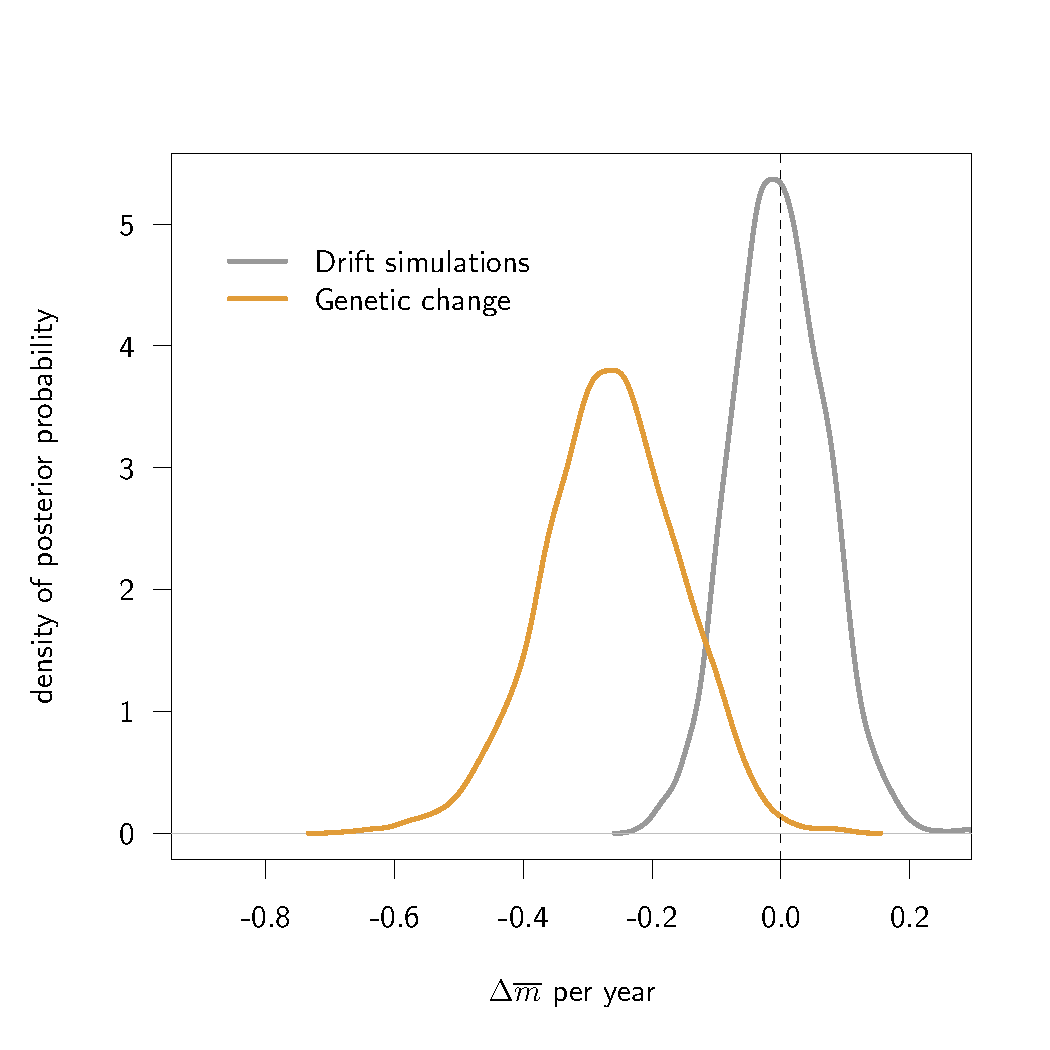
\includegraphics[width=0.5\textwidth]{FiguresStasis/Drift-1}
\caption{\footnotesize \textbf{Estimation of the rate of genetic change and rate of change expected under drift.} The posterior distributions of the realized rate of genetic change, estimated by the Price equation, exceeds that expected under genetic drift $p=0.009$.}
\label{fig:drift}
\end{figure}

\begin{figure}[ht]
\centering
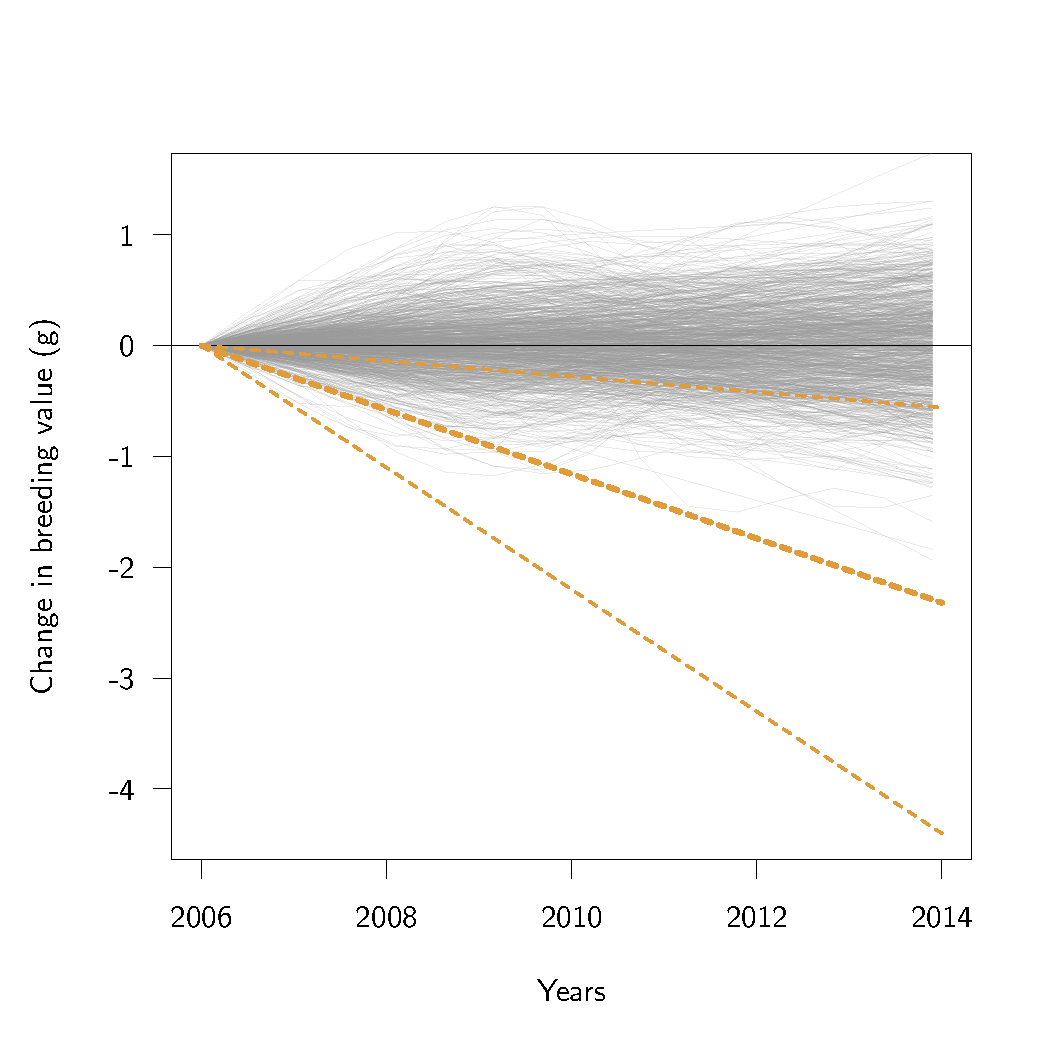
\includegraphics[width=0.5\textwidth]{FiguresStasis/DriftComp-1}
\caption{\footnotesize \textbf{Estimation of the time-trajectory of genetic change and evolutionary trajectories simulated with drift only.} Evolution of breeding values for mass are shown relative to the year 2006. The yellow lines show the mode and 95\% credibility interval of the rate of evolution estimated by the Price equation within an animal model. The gray lines show 1,000 simulations of genetic drift, based on the real population pedigree and on the posterior distribution of genetic variance for mass estimated by the animal model. The probability that the observed rate of evolution happened due to drift is only 0.009, less than could be understood from the overlap between the two distribution. It is, however important to notice that the two distributions are not independent, but that small (/large) values of change due to drift are simulated for small (/large, respectively) posterior samples of estimate rate of evolution.}
\label{fig:driftcomp}
\end{figure} 


\begin{figure}[ht]
\centering
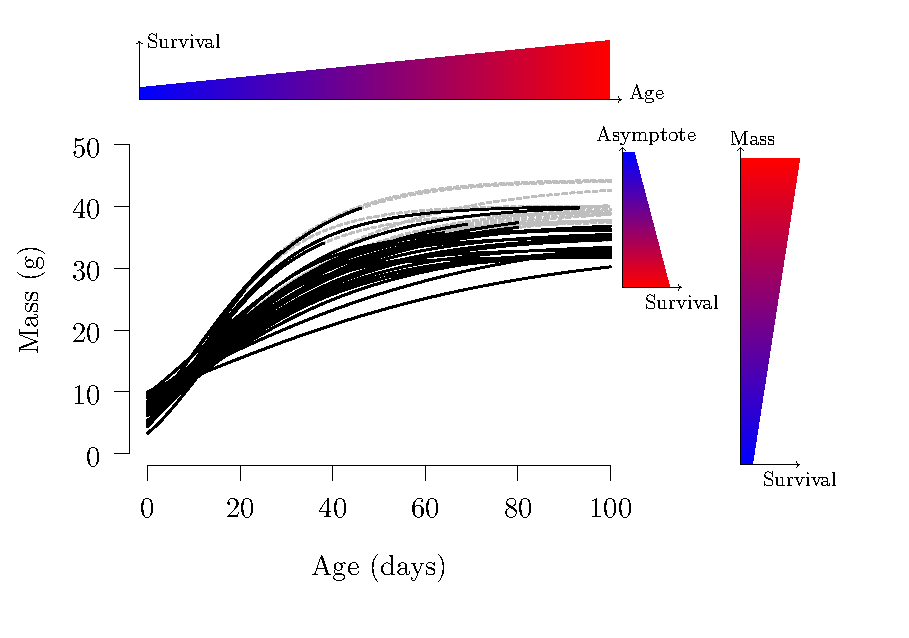
\includegraphics[width=\textwidth]{FiguresStasis/schemeSelectionAM}
\caption{\footnotesize \textbf{Conceptual illustration of the selection for asymptotic mass despite apparent selection for mass.} Black lines represent simulated individual growth trajectories, and they are prolonged by grey dashed lines after an individual death. The probability of surviving between the time of measurement and the next year increases with age. Because mass increases with age, there is apparent selection favouring heavier individuals. However, it is still possible for viability selection at a given developmental stage, such as asymptotic mass, to be negative. Because genetic variation is related to asymptotic mass, but not to age, the expected genetic change will be toward lower masses.}
\label{fig:scheme}
\end{figure}
%\end{refsection}
%
%
\begin{refsection}
\chapter[Fluctuating selection]{Fluctuating selection}
\end{refsection}
%
\begin{refsection}
\setchapterpreamble[ur][.6\textwidth]{%
\dictum[Miyamoto Musashi, \textit{A Book of Five Rings} (circa 1645)]{%
It is difficult to understand the universe if you only study one planet.}\vskip1em
}

\chapter[\texorpdfstring{Chapter 6 \\ General discussion}{Chapter 6 General discussion}]{General discussion}
\chaptermark{General discussion}
\label{chap:discu}

\section{Overview}
In this thesis, I investigated the causes and consequences of variation in fitness in a wild population. I showed that the variation in proxies for individual fitness is not purely stochastic, but is underlain by variation in latent fitness (chapitre \ref{chap:dynhet}). Besides, the variation in latent fitness has an additive genetic component, showing the presence of natural selection and of adaptive evolution in the snow vole population (chapter \ref{chap:stasis} and \ref{chap:flusel}).
I explored ways to decompose the causes of phenotypic changes and identified the animal model from quantitative genetics as a convenient tool to estimate evolution (chapter \ref{chap:decpop}).
Using this tool in various ways, I showed that body mass was an important contributor of variation in fitness proxies (chapter \ref{chap:stasis}), but not in a consistent way over time (chapter \ref{chap:flusel}). Nevertheless, body mass was a consistent contributor to variation in genetic variation for fitness (chapters \ref{chap:stasis} and \ref{chap:flusel}), and therefore, body mass evolved over the study period.

Below, I will discuss further the insight brought by this thesis and the remaining challenges, in understanding the causes of phenotypic variation and the response of wild populations to environmental change. 

\section{The causes of phenotypic variation}
This thesis brings some new knowledge about the causes of variation in fitness and other phenotypes, but there is still much more to learn. Causality can be refined \emph{ad infinitum} unless, perhaps, once phenotypic variation is modelled in term of quantum interactions between fundamental particles. Below, I comment on two promising directions that were only touched upon in this thesis, but have the potential to improve the predictive understanding of the causes and consequences of fitness variation. These are the effect of an individual's gene on other individuals, and the study of the molecular basis of genetic variation through genomics.

\subsection{The effect of others' genes}
Using quantitative genetics, I decomposed the phenotypic variation of morphological and life-history traits into components related to additive genetic effects, maternal effects or permanent environments. This decomposition was sufficient to measure the rate of evolution of the direct genetic effects (chapter \ref{chap:stasis}), that is, the direct action of an individual's genes on its own body.
Nevertheless, an individual's genes have effects reaching out beyond its body, to the environment, including other individuals \parencite{Dawkins1982}, whether it is through interactions between individuals (indirect genetic effects, e.g. maternal effects, \cite{McAdam2014}), or through the pleiotropic action of genes expressed in kin at different life-stages (e.g. genetic conflicts, \cite{Trivers1974}).

Indirect genetic effects could be an important component shaping selection and evolution in the snow vole population. Indeed, in the snow voles, genes within an individual are likely to affect the phenotype of another individual during at least two types of situations. First, related females tend to form clusters of territories, and the presence of kin could suppress reproduction in subordinate females \parencite{Garcia-Navas2016}. Moreover, as in all placental mammals, maternal effects on offspring phenotypes are prevalent from pregnancy to weaning. 
Maternal effects have been studied extensively in natural populations \parencite{Wolf2009}, but estimations of the genetic component of maternal effects remain scarce \parencite{McAdam2014}. Nevertheless, genetic maternal effects could provide extra evolutionary potential in addition to that of direct genetic variation \parencite{Mcglothlin2014, McAdam2014, Mcfarlane2015}. In the snow vole population, preliminary analyses showed the presence of additive genetic maternal effects for body mass (results not shown). Genetic maternal effects for mass could therefore be subject to selection and evolve adaptively. In chapter \ref{chap:stasis}, maternal genetic effects are not explicitly modelled, and their evolution is assigned to phenotypic plasticity. A full account of body-mass evolution should measure this evolution in addition to that of direct additive genetic effects. 

Besides indirect genetic effects, the effect of others' genes matters for evolution in the case of genetic conflicts, that is, genetic trade-off between traits expressed in different individuals.
For four decades, genetic conflicts between parents and offspring have been thought to be a major constraint on the evolution of size \parencite[since][]{Trivers1974}, but the idea resisted empirical tests despite behavioural studies showing patterns consistent with it \parencite{Kolliker2015}. \cite{Kolliker2015} demonstrated that a genetic trade-off between offspring number and offspring size constrains the evolution of size in earwigs (\textit{Forficula auricularia}, Linnaeus 1758). Moreover, \cite{Rollinson2015b} presented qualitative evidence suggesting that this constraint is widespread among animals and could be a general explanation for the evolutionary stasis of size. 
In chapter \ref{chap:stasis} we briefly explored the possibility that a genetic conflict constrains the evolution of body mass, and found qualitative evidence that it is not the case. The snow vole study system is not an ideal to test this hypothesis, however. First, we do not capture all juveniles\textemdash some die or emigrate before their first year\textemdash and cannot measure litter size accurately. Because mass is under selection in juveniles, selective disappearance is likely to blur the trade-off signal \parencite{Hadfield2011}. Second, the size-number genetic trade-off is best described as an explanation of evolutionary stasis of size or mass, but mass is evolving in the snow vole population (chapter \ref{chap:stasis}), making it more difficult to formulate an expectation for the genetic covariance between mass and litter size. 
Finally, it is in theory possible to measure the genetic trade-off using quantitative genetics, but nor the exact model to fit nor the modelling tools are published yet \parencite{Hadfield2012, Rollinson2015b}. An experimental approach remains the only option to quantitatively test for a size-number genetic trade-off \parencite{Kolliker2015}, and such an approach appears impossible in a wild population such as Churwalden's snow voles. 

\subsection{Molecular basis of genetic variation}
During this PhD, on several occasions, Dr Erik Postma and myself, considered using high-throughput genome sequencing \parencite{VanDijk2014} to sequence the snow vole population retrospectively (tissue is kept in $-80^\circ$ freezers for most of the individuals trapped in the last ten years).
As of yet, we did not obtain the funding necessary, and I ran out of time to carry out work in the laboratory and to develop a bio-informatic pipeline. 
As I discussed in chapter \ref{chap:intro}, molecular approaches to measuring selection and evolution are in general inferior to quantitative genetic approaches. Nevertheless, individual-based genomic data could bring complementary insights to my empirical chapters.

To start with, individual-based genomic data could marginally improve the estimation of quantitative genetic parameters \parencite{Berenos2014} by: (i) allowing the use of realized relatedness in animal models, instead of the relatedness expected from the pedigree; and (ii) providing some relatedness information about individuals with unknown parents (for which there is no information at all in a pedigree). 
More importantly, individual-based genomic data would allow the identification of some of the genetic loci underlying phenotypic variation and quantitative evolution.
This task is generally a challenging one in small populations \parencite{Wellenreuther2016}, but the snow vole population presents three rare advantages that would ease it considerably. 

First, at least one trait, body mass, has been evolving during the last decade, and some adaptive molecular evolution must have happened. The search for the molecular basis of evolution would therefore start with the knowledge that there is something to find, and with indications on what functional types of genes are likely to be involved. 
Second, in natural populations, it is difficult to show that evolution at a genetic locus is due to selection and not only due to drift, because there is in general no null-expectation for the effect of drift under complex demographics and mating patterns. A pedigree provides such a null expectation. Simulating the random dropping of alleles down our pedigree would results in a null distribution of changes in allele frequencies against which to test for the effect of selection on each genetic locus. This method was successfully employed to show contemporary adaptive evolution at 67 genetic loci in a wild population of Florida scrub-jays (Nancy Chen, Evolution conference, 2016, Austin, USA).
Third, thanks to the availability of life-history data, it would be possible to correlate the allelic variation of the evolving loci to success and failure in various life-stages.  
Therefore, the combination of genomic and life-history data can pinpoint when selection occurs in life, and what kind of molecular mechanism selection acts on.
Altogether, individual-based genomic data could therefore refine not only our molecular understanding of phenotypic variation, but also provide clues regarding the ecological nature of selection. 

%\subsection{Origin and maintenance of variation in fitness}
%%fondamental maintenance of g var
%Still, our study is a snapshot, too short to expect significant loss of genetic variation. What would happen if the observed selective pressures would carry on? 
%Fluctuating selection might contribute to the maintenance of genetic variation
%New mutations certainly contribute, but probably not sufficient in general (charlesworth).
%Population structure. 

\section{Predicting responses to environmental change}
Anthropogenic environmental change has triggered research aiming at understanding and predicting the response of natural populations to environmental change \parencite{parmesan2006, Chevin2012, Smallegange2013, Charmantier2014climate}, but massive challenges hinder this research agenda. Already, the retrospective study of phenotypic and demographic responses often remains inconclusive \parencite{Merila2001,McCarty2001, Charmantier2014climate, Brookfield2016} and, at the moment, prospective prediction seems out of reach in most cases. 
During my Ph.D., I confronted three challenges that must be tackled to improve the predictive abilities of evolutionary ecology. Below, I discuss the problems with measuring selection, predicting the response to selection, and integrating evolutionary and demographic responses.

\subsection{Measuring selection in the wild}
For over 150 years, natural selection has been known to cause the match between organisms and their environment, and biologists have attempted to understand its causes and mechanisms. More recently, the study of selection assumed a more applied goal as researchers hope to predict the response of natural populations to the selective pressures imposed by environmental change \parencite{Chevin2010a, Coulson2010, Merila2014}.
The principle of natural selection is very simple: in a given environment, individuals with a phenotype that favours survival and fertility contribute more to the next generation. Given the level of research attention on such a simple process, it can be surprising to see how slowly the understanding of natural selection has developed, and how difficult its study remains. 
For most of the 20th century, the main brake to progresses was the lack of an unified framework to quantify selection in natural populations \parencite{Wade2006}. Such a framework progressively emerged, starting with covariance-based methods \parencite{Robertson1966, Price1970} which efficiently measure the total effect of selection. The most influential breakdown was the popularization of regression-based methods \parencite{Lande1979,Lande1983} which measure the proportional effect of selection per unit of phenotypic variation, and allows to decompose selection into the direct and indirect effects of selection on multiple traits \parencite{Broodie1995}.
Since then, these methods have provided thousands of estimates of selection in natural populations \parencite{Kingsolver2001,Stinchcombe2008,Kingsolver2012}, thus showing several general patterns. For instance, directional selection is stronger and more common than suggested by early evolutionists, whereas stabilizing selection appears to be rare, while fertility selection is generally stronger than viability selection \parencite{Kingsolver2012}.
The abundance of estimates of selection should not be mistaken for a good understanding of natural selection, however. The estimation of selection through regression-methods faces at least three difficulties that might severely hamper their significance and explain the general absence of response to selection \parencite{Merila2001, Brookfield2016}.

First, to obtain an unbiased measure of selection, fitness should be regressed on the trait of interest. Since, fitness is rarely observable directly, fitness proxies must be used instead. Many estimates of selection are computed on fitness components, for instance fertility and survival \parencite{Kingsolver2012}. In this case, the estimation of selection can be biased in the presence of a trade-off between fitness components: a certain phenotype might increase survival but decrease fertility, so that the net selection on the trait is null, despite covariation with fitness components \parencite{Thompson2011, Kingsolver2012, Brookfield2016}. Fortunately, this bias appears to be minor in general, with the exception of body mass \parencite{Kingsolver2011}.
For the empirical part of this thesis (chapter \ref{chap:stasis} and \ref{chap:flusel}), I used fitness proxies that attempted to include all fitness components in order to avoid a bias. Thus, I used lifetime reproductive success when measuring selection within a generation, and annual reproductive success plus twice survival when measuring selection within a year. These fitness proxies are imperfect since we do not capture all juveniles and a trade-off between early juvenile survival and reproduction could bias the selection estimation \parencite{Hadfield2008}. Still, estimates of evolution using Price equation (that is, selection on the genotype) or using the trend in BLUPs for breeding values (that is, not using any information about selection nor fitness) agree qualitatively with my corrected estimates of selection (chapter \ref{chap:stasis} and \ref{chap:flusel}), suggesting that my proxies for fitness are adequate. 

Second, it is possible to estimate the total effect of selection on a trait with selection differentials, but it is much more difficult to disentangle the causal selective effect of a trait from the indirect selection due to other traits. In theory, it is possible to disentangle direct and indirect selection by including all the traits under selection in the analysis \parencite{Lande1983}. In natural populations, however, it is impossible to know \emph{a priori} what traits are under selection, and often it is impossible to measure all relevant traits \parencite{Brookfield2016, Hadfield2008}. Furthermore, as more traits are included in a selection analysis, the statistical power to detect significant selection on any one trait decreases \parencite{Mitchell-Olds1987}.
I did detect significant indirect selection on body mass, but genetic correlations between the traits considered were such that the prediction of evolution was not affected by the inclusion of indirect selection (chapter \ref{chap:stasis}). Only three traits were tested, however, and we cannot exclude that body mass is not under indirect selective pressure. The evolution of body mass could be driven by selection on an unmeasured trait.
Nevertheless, this problem is irrelevant to the measures of total selection and evolution, on which chapters \ref{chap:stasis} and \ref{chap:flusel} rely.

Third, covariance-based and regression-based methods to estimate phenotypic selection essentially measure the statistical association between traits and relative fitness. Selection must however be a causal association, be it direct or indirect. If the statistical association is entirely mediated by an environmental covariance between traits and fitness, there is no selection and no possibility of genetic response to selection \parencite{Price1989, Rausher1992}. 
Body mass, the main trait analysed in this thesis, is likely to be very sensitive to this source of bias. Indeed, a favourable environment\textemdash for instance food rich and lacking parasites\textemdash is likely to lead to larger mass, high survival, and high fertility. Accordingly, phenotypic estimates of natural selection on mass and size are overwhelmingly positive, but mass does not evolve has predicted from its heritability \parencite{Blanckenhorn2000, Kingsolver2012}. In the snow voles, an excess of environmental covariance does underlie the apparent selection on mass (chapter \ref{chap:stasis}).
A solution to the problem is the experimental manipulation of the trait of interest. This can break the link between phenotype and individual quality and reveals the causal action of phenotype on fitness components \parencite[e.g.][]{Tinbergen2004, Tschirren2006}. Still, experimental manipulation is no without its own limitations.
Thus, manipulations are work intensive, time consuming and must be designed carefully in order to manipulate the trait of interest without affecting any other trait. Moreover, manipulations cannot easily be applied to all traits. The approach has been widely used to study selection on brood size, but it is not clear to me how one could manipulate body mass in a controlled way (that is, without accidentally affecting other traits).
Instead of an experiment, my approach to the challenge of environmental covariation has been to use quantitative genetics to identify the target of natural selection (chapter \ref{chap:stasis}). After having shown on-going adaptive evolution, I decomposed phenotypic selection into an additive genetic and an environmental component, for various fitness components. I found that only juvenile viability selection showed an additive genetic component, and according to the Robertson-Price identity, was the source of adaptive evolution. Understanding the mechanism of this selection and measuring its strength was then a matter of hypothesis testing.
This approach could be used on other systems provided the presence of adaptive evolution. Nonetheless, it requires sufficient phenotypic and relatedness data to fit bivariate animal models. In addition, in the snow vole a single fitness drove evolution, but multiple fitness components could be involved, thus complicating the analysis. Finally, identifying the right fitness component(s) does not guarantee that the phenotypic mechanism of selection can be identified. A good understanding of the biological system will be necessary to formulate a reasonable hypothesis for the cause of selection. The testability of this hypothesis will also depend on data availability and quality, and will be subject to the limits of hypothesis testing approaches: there is always a risk of false positive, equal to the significance level chosen for the test, and a correlation does not prove causation.


\subsection{Evolutionary response}
Once a measure of phenotypic selection is obtained, it is straightforward to formulate a prediction of genetic response based on the breeder's equation and on a heritability estimate \parencite{Lush1937, Falconer1996}. We have already seen (chapter \ref{chap:stasis} and \ref{chap:flusel}) that such a prediction is often unreliable in natural populations, however.  Estimates of selection might not correspond to causal selection, and unmeasured selection acting on genetically correlated traits might constrain evolution. I have shown that estimating the genetic component of selection, or the rate of evolution, can test whether selection has been measured appropriately to be predictive (chapter \ref{chap:stasis}). 

Nevertheless, most attempts to understand the evolutionary response to environmental change do not measure genetic parameters. Thus, the alarming lack of evidence for evolutionary responses to climate change probably originates primarily from a lack of tests for genetic change \parencite{Charmantier2014climate,Gienapp2014,Merila2014,Crozier2014}.
Ignoring the genetic properties (e.g. the heritability) of the trait of interest \parencite[e.g.][]{Forcada2014, Coulson2014, traill2014demography} easily leads to underestimating, or incorrectly dismissing, the potential to respond to selection and the actual evolutionary response \parencite{Nietlisbach2015, Chevin2015a, Pigeon2016}.
Similarly, the evolutionary potential of small populations was dismissed by population matrix simulations that ignored genetic-based arguments (see chapter \ref{chap:dynhet}). Moreover, methods based on phenotypic covariances do not distinguish between the presence and the absence of heritable variation, and cannot be used alone to predict an evolutionary response (chapter \ref{chap:decpop}).

Therefore, all the chapters of this thesis illustrate that a genetic approach, be it based on quantitative genetics or population genetics, is necessary to measure evolution, and can more reliably identify the selective causes and the constraints shaping adaptation. 
Attempts to understand the evolutionary dynamics of natural populations based on phenotypic observations only \parencite[e.g.][]{Smallegange2013} are a gamble, that might work on special occasions, but is unlikely to be reliable in general. 

\subsection{Demographic response to environmental change}
This thesis is almost exclusively concerned with traits and their evolutionary dynamics. 
In the context of understanding the response of natural population to environmental change, such an investigation is legitimate. Whether a trait distribution changes through demographic, plastic, or genetic mechanisms has different consequences on the fate of the population \parencite{Chevin2010}.
Nevertheless, for most applications, and to the eyes of the society, it is unimportant whether animal and plant populations respond to climate change primarily through migration, through plastic changes, or through evolution. The primary motivation of this research is to ascertain whether populations will persist or go extinct, and how managers can affect the outcome.

This question is primarily a demographic one. The evolutionary approach that was mine during this PhD is not sufficient to ascertain the fate of the snow vole population, but it might be a useful first step. Indeed, it is now widely acknowledged that evolutionary processes can act on the same time scale as ecological ones, and that they can significantly affect demographics \parencite{Hairston2005,Ellner2011, Chevin2010a, Turcotte2011}. For instance, theory and laboratory experiments support the existence of \emph{evolutionary rescue}, that is, adaptive genetic change within a population that prevent the population extinction \parencite{Gonzalez2013a, Schiffers2013a}. Still, empirical evidences of evolutionary rescue in the wild remain extremely limited \parencite{Wal2013}.

In chapter \ref{chap:stasis}, I inferred that the genetic response to selection tended to increase mean juvenile survival over the study period. All other things being equal, evolution therefore had a positive demographic effect and contributed to the recovery of population size. It is, however, unclear to me how to quantify the demographic effect of evolution. To the best of my knowledge, an appropriate methodological framework is still lacking. 
Indeed, traditional demographic models used to predict population resilience ignore individual heterogeneity and genetic change \parencite{Kendall2011, vindenes2015, Plard2016}. On the other hand, quantitative genetic studies focus on estimating rates of evolutionary change, but mostly ignore their possible consequences for the dynamics of populations \parencite{Coulson2010,Chevin2012}.
It is now acknowledged that the integration of evolutionary and demographic aspects is crucial for predicting trait dynamics, population resilience and viability \parencite{Schoener2011,Pelletier2012,Chevin2012,Merila2014}. But only in the last year have publications proposed methods that could start to address this question in the wild \parencite{vindenes2015, Coulson2015, Childs2016}, and these should certainly been followed up. 

\section{General conclusion}
Natural selection is a potent force that shapes the evolution of natural populations, but its causes and consequences can be blurred by the complexity of natural populations.
Understanding the process of adaptation requires to isolate selection from the stochasticity in fitness components, to disentangle evolution from other drivers of phenotypic change, and to mechanistically link genetic change to selective pressures.
Being able to do so, thanks to an individual-based monitoring including genetic relatedness, I provided a rare example of contemporary adaptive evolution. More examples of evolution in action certainly await to be described, and will make our understanding of the response to environmental change more general and more predictive. This thesis, however, shows in several ways that crucial insight is more likely to come from studies that explicitly study the genetic aspects of selection and phenotypic changes.


\printbibliography[heading=subbibliography]

\end{refsection}

\setchapterpreamble[ur][.6\textwidth]{%
\dictum[J.R.R. Tolkien, \textit{The Fellowship of the Ring}]{%
I don't know half of you half as well as I should like; and I like less than half of you half as well as you deserve.}\vskip1em
\dictum[Roman Kacew, dit Romain Gary, La Promesse de l'aube]{
Je feins l'adulte, mais, secr\`etement, je guette toujours le scarab\'ee d'or, et j'attends qu'un oiseau se pose sur mon \'epaule, pour me parler d'une voix humaine et me r\'ev\'eler enfin le pourquoi du comment.}\vskip1em
}

\chapter{Acknowledgments}

Looking back to one's life, it is amazing to notice how much the path it took has been influenced by a myriad of people. These acknowledgments are about a PhD thesis, but they are bound to look back in time far beyond the PhD onset.

First and foremost, many thanks to Erik Postma for being such a great supervisor. Erik set the track for a fascinating and successful PhD project when he realized the potential of the snow vole monitoring and wrote a thoughtful NSF proposal full of surprisingly correct guesses about the biology of the population. Erik taught me statistical techniques, ideas from quantitative genetics and presentation techniques. More importantly, though, he trained me to consider logical arguments critically, read scientific publications in depth (in particular during epics journal clubs that ended up ``rejecting'' more than half of what we read based on technical or logical flaws) and thus learn from the mistakes of others, to learn a bit less from mine. For four years, Erik's door was literally \emph{always} open (I cannot recall a time when he did not have some time to discuss) to answer my ``little questions'' and review my work.
Finally, it impossible not to mention that Erik introduced me to running, pushed me to run more often, longer and faster, and thus kept me fit, healthy and entertained.

Not being one of his students, and given his very tight schedule, I am especially grateful to Lukas Keller for long conversations, old paper mining and spontaneous suggestions. His seemingly encyclopaedic knowledge, and his almost as rich library, not only solved a few crucial issues relevant to my PhD, but also kept acute my appetite for the wonders of population genetics, organismic biology and statistics. 

%rest of the committee
Thanks to Arpat Ozgul for his constant enthusiasm about the project and for supporting its continuation during the postdoc to come. Also, thanks for being a bridge to the ideas and slang of population ecology and demography, thus clarifying ``translation'' issues. 

Thanks to Barbara Tschirren for her precious suggestions when trying to understand the voles in a more mechanistic way, molecular and physiological. Thanks for letting me take your brand new respirometer in the humidity, low pressures and shakiness of the field. 

The most important analyzes of my PhD were run with the package \texttt{MCMCglmm}, and I was extraordinarily lucky to count his creator, Jarrod Hadfield, among my committee members. Besides technical support, Jarrod helped clarifying some confusing concepts and results from quantitative genetics. Also, thanks to him for giving me the opportunity to review for the journal Evolution. 

Thanks to Marc K\'{e}ry for his help and encouragements with complicated JAGS models, but also for some sound life-planing advice. 

Thanks to Peter Wandeler for initiating the snow vole monitoring in Churwalden, while I was still a high-school student, unaware of the scree little happy folks. 
% Zurich people and related
%office

I could never thank enough Glauco Camenisch for the help he provided in the lab, on the field, in front of the computer and in the kitchen. Glauco saved me many weeks of work and made constant efforts to improve the quality of data set. He would deserve to be awarded a good share of this PhD.
With Glauco, the other backbone of the research group is Ursina Tobler. 
Ursina always keeps the administrative duties minimal on our side, but makes sure everything works fast and smoothly in the background. Thanks to her for making the live of students so easy. 

%Co-authors and field helpers
During the last three years, the majority of my scientific discussions were with Koen van Benthem. I am grateful for his many ridiculous questions and discoveries, most of them turned out to be puzzling or insightful. A particular thank for pushing me towards \LaTeX and Zurich Tonhalle. 
I wish he will one day understand the pattern behind prime numbers, and bring more mathematical rigor into ecology and evolution. 
Thanks also to him for taking the lead (i.e. first first authorship or sixth last authorship) on our ``Price's equation review'' (from which Price's equation was eventually extirpated), a long and tedious, but incredibly educational, collaboration, for which I also have to thank Marjolein Bruijning and Eelke Jongejans.

Vicente Garc\'ia-Navas can do research faster than a snow vole can run into a trap, and he publishes it in good journals before the apple is all eaten. It was very stimulating and good for my CV to work with him. 

Andres Hagmayer was an exemplar Master student, very serious, autonomous and efficient. Thanks to him for almost two years of a fruitful collaboration that taught me a lot about teaching. 

Thanks to Cindy Canale for helping with respirometry, for kind encouragements and nice parties. 
Many thanks to Dominique Waldvogel and Martina Schenkel for precious and cheerful help on the scree. 


For four years, the majority of my non-sleeping time was spent in the company of the ``permanent residents'' of the office Y13-J-34. I will remember this office as home (although I kept my word and never spent a night there!) thanks to all our passionate discussions, our ire at wrong papers, our debugging struggles and our coffees breaks. Special thanks to Pirmin Nietlisbach for hosting me on Mandarte island; to Philipp Becker for teaching me how to cross-country sky and how to catch dippers; and to Judith Bachmann for nice frog expeditions. 
This office was such a great place to work, live and laugh with the essential contribution of its intermittent occupants,
Erica Ponzi, 
Vanja Michel, 
Rien van Wijk and 
Johann Hegelbach.

%Inspiring relationships

Thanks to the Kokonuts\textemdash Hanna Kokko, Isobel Booksmythe, Ana\"is Tilquin, Nina Gerber, Susanne Schindler and Xiang-Yi Li\textemdash for inspiring journal clubs, where you can sit on an orange primitive salamander (definitely not a pony).
Christine Grossen and Daniel Croll are among the kindest humans I have ever met. In particular, thanks for welcoming me during my first days in Z\"urich and for lending me a piano for two years.
Merci to Chelsea J. Little for being a great adventure buddy, a cheering friend and an example of scientific brightness. 

Many thanks (sadly impersonal so that the acknowledgments do not become a thesis chapter on their own right) to the Z\"urich folks for four very fun and enriching years. In a jumble, thanks to 
Alexandra Jansen van Rensburg 
, Alexander Nater
, Irene Weinberger
, Simon Evans
, Jasmin Winkler
, Joel Pick
, M\'elissa Lemoine
, Dennis Hansen
, Stefanie Muff
, Rassim Khelifa
, Debbie Leigh
, Josh van Buskirk 
, Kasia Sluzek
, Fr\'ed\'eric Guillaume
, Béatrice Nussberger
, Benedikt Gehr	
, Nina Vasiljevic
, Ulrich Reyer
, Hedwig Ens
, Wolf Blanckenhorn
, Tina Cornioley
, Sam Cruickshank
, Mollie Brooks
, Juan Pablo Busso
, Franziska L\"orcher
, Jobran Chebib
, \emph{Cini} Gabriella Gall
, Andreas Sutter
, Aur\'elie Garnier
, Nino Magg
, Inge Juszak
, Gianalberto Losapio
\dots

Special thanks to Ashley E. Latimer for forcing me to cook and go birdwatching during stressful periods, for teaching me some English and for inspiring conversation bridging gaps between population genetics and evolution over geological timescales. 

%Scientific early experiences
I never had the opportunity to thank all the great people I have met since the beginning of my scientific life (because I didn't write a report for the two first internship, and acknowledgments were \textit{prohibited} (sic) for my master thesis). Still, I owe them a lot, and many people were instrumental in setting the path toward a PhD. 
In 2011, while I was trying to \sout{escape from} leave engineering for fundamental research, without having much clue of what it was about, Jean-Fran\c{c}ois Martin gave me the opportunity to give it a try by tutoring a gap year entirely dedicated to research. Pierre-Andr\'{e} Crochet provided determinant help to find my way in the cloud of biology and reach a first research experiment, in the form of an internship at University of Oslo CEES. There, Glenn-Peter S{\ae}tre was an amazing first supervisor, extremely patient with my childish English, my misadventures in the lab and my perfect ignorance in evolutionary genetics, and was very supportive to find housing and survive one semester in Norway without any income. Thanks to him and all his team, especially Tore Oldeide Elgvin and Anna Fijarczyk, I had a great time that convinced me that fundamental research in evolutionary biology would be a good way to spend my time. This might be where I learned the most about what the life of an evolutionary biologist was about: from sequencing DNA, to searching and understanding scientific literature; from the quasi-universal fascination of scientists for coffee and Friday beer, to the poetic insight of Kimura's neutral theory, and many more things. Eventually, thanks to them for making me publish my first research papers, although I did not do a lot and was probably not really understanding the little I did. 
I then went to Chiz\'{e} CEBC where I worked with a crew of amazing people including Adrien Pinot, Vincent Bretagnolle, David Pinaud, Vincent Lecoustre, Edoardo Tedesco, thanks to them and all the other Chiz\'eens for all they taught me. A particular thank to Mathieu Authier for his (partially-successful) attempt to convert me to Bayesianism, and to Laurent Crespin for forcing me to go deeper into Mark-Recapture modeling and maximum of likelihood. Last but not least, Bertrand Gauffre was crucial in my scientific development, thanks to him for our many conversations, for taking me seriously, for introducing me to Richard Dawkins' writings and for pushing me to do complete my Masters in Montpellier. 
The B2E Master in Montpellier was a time of hard studying, and great fun, during which some teachers opened my mind to new scientific horizons, thanks in particular to Patrice David, Isabelle Olivieri, Olivier Gimenez and Michel Raymond for that.
Thanks to Rapha\"{e}l Leblois for introducing me to the coalescent theory and its powerful thought experiments, as well as to \texttt{C++} programming. Coding \texttt{ForwardBackward} and its improved sequels was a crazy adventure, full of traps and wonders. Thanks to Fran\c{c}ois Rousset for giving me a small sight at what it means to understand population genetics, statistics, logic and the world in general.
Thanks again to PAC for his patient help explaining me again and again evolutionary concepts and writing tricks.
Also, thanks to Nicolas Bierne for his PhD offer and our fascinating discussion on oceanic streams, gene flow and the elusive eel, I still think about this alternative scientific and life path with curiosity and envy. 

Thanks to all the Montpellierains, in particular \'{E}meric Figuet, L\'{e}o Grasset, Joane Elleouet, Paul Sanders, Pascal Milesi, Julie Landes\dots our conversations account for of what I know in evolutionary biology.
%My muses
Out of the academic world, I could always count on the support of Ga\"elle Jeanne Duranthon during the last 12 years. Thanks also to my two adoptive families who kept me cheerful with meals, games, music, remote places, short nights and craziness during the last decade. These are the Goret family with an otter, a weasel, a canary, a baboon, a snail, a goat, a bee, a goose, a panda, a wolf, a bear, an owl, a lion and a chameleon; and the Margicon (\copyright \textit{une marque d\'{e}pos\'{e}e par terre}) family: Nounou, Chonchon, Caca, Doudou, Mirabelle and their mates/cats/penguins.

My early interest for ecology and evolution was much reinforced by wandering across the forests, meadows and moorlands of Lacaune mountains, by the contemplation of glittering and diverse carabids, by the excitement of long days monitoring bird migration, by astonishing conversations on conservation and nature management and by the constant realization that while we still know so little, it takes only some sweat and patience to discover new things.
This early encounter with life would have not been sustainable without the naturalists who taught me so much and kept me amazed. Thanks in particular to Amaury Calvet and other members of the ``Ligue pour la Protection des Oiseaux du Tarn'' as well as to the members of BeaOsea: Adrien Chaigne, Camille Denozi\`{e}re, Aur\'{e}lien Salesse, Denis Guillaumin and Manon Ghislain.

Some high school teachers were particularly influential not so much by what the taught, but rather by how they taught to learn, to see things in another way or by opening unexpected opportunities. Many would deserve acknowledgments for doing that at diverse degrees, but here are a few whose classes remain very alive: Beno\^{i}t Leviandier, Mdm Rolland, Jacky Cariou, Jean Leblanc.

Being born in such a family made life rather easy. Thanks especially to my parents Francine and Claude, to my siblings Kiyomi-\'{E}lodie and Cyrille, to my grand-parents Juliette, Louis, Andr\'{e} and Simone and to my uncle Laurent. They kept supporting, sustaining and trusting me over long years of studies they could less and less understand.
\chapter[Curriculum Vitae]{CV Timoth\'{e}e Bonnet}
%\textit{PhD student in evolutionary biology}\bigskip\par}} 

\section{Personal Data}
\begin{tabular}{p{4cm} p{11cm}}
\hfill \textsc{Birth date:} & November 1st 1988\\
\hfill \textsc{Nationality:} & French\\
\hfill \textsc{Work address:} & Department of Evolutionary Biology and Environmental Studies\\ 
									& University of Z\"{u}rich\\
									& Winterthurerstrasse 190\\
									& CH-8057 Z\"{u}rich\\
									& Switzerland \\
\hfill \textsc{Phone:} & +41 (0)44 635 47 66\\
\hfill \textsc{email:} & \href{mailto:timothee.bonnet@ieu.uzh.ch}{timothee.bonnet@ieu.uzh.ch}\\
\hfill \textsc{Personal page} & \url{http://www.ieu.uzh.ch/staff/phd/bonnet.html} \\
\hfill \textsc{Languages:} & French (mother tongue), English (fluent), Spanish (basic)
\end{tabular}
\vfill


\section{Education}
\begin{tabular}{r|p{11cm}}
\textsc{Oct 2012 -} \emph{Current} & \textbf{PhD student in Z\"{u}rich evolutionary biology PhD program.}\\
								& \emph{Individual-level causes and population-level consequences of variation in fitness in an alpine rodent.}\\ 
								& \footnotesize{Under the supervision of Dr Erik Postma.}\\
\textit{Courses:} & \\
\footnotesize{\textsc{May 27-28}th 2013}& NGS for Model and Non-Model Species, by K. Shimizu \& al.\\
\footnotesize{\textsc{Jun 22-29}th 2013}& Evolutionary Biology Workshop in Guarda, by D. Ebert \& S. Bonhoeffer\\
\footnotesize{\textsc{Oct 10-11}th 2013}& Workshop on Integral Projection Models, C. Merow \& al.\\
\footnotesize{\textsc{Oct 14-18}th 2013}& Evolutionary Demography, by D. Levitis \& al.\\
\footnotesize{\textsc{Jan 13-17}th 2014}& Bayesian Population Analysis using WinBUGS, by M. K\'{e}ry \& M. Schaub\\
\footnotesize{\textsc{Nov 6-7}th 2014}& Advanced Software Carpentry, by M. D. Robinson \& al.\\
\footnotesize{\textsc{May 18-19}th 2015}& Advanced NGS, by S. Wider \& H. Lischer\\
\multicolumn{2}{c}{} \\

%------------------------------------------------

\textsc{Sep 2011 - Jun 2012} & \textbf{M.Sc. in evolutionary biology and ecology. University Montpellier II, France.}\\
\textit{Research project:} & \emph{Neutral processes and biased mitochondrial introgression} at the center for population biology and management (CBGP).\\
& \footnotesize{Supervised by Drs Rapha\"{e}l Leblois, Pierre-Andr\'{e} Crochet and Fran\c{c}ois Rousset.}\\
\multicolumn{2}{c}{} \\

%------------------------------------------------

\textsc{Sep 2008 - Sep 2011} & \textbf{B.Sc Biology: National engineering school in biology and agronomy, Montpellier Supagro, France.}\\
& \footnotesize{Specializations in biodiversity conservation, ecology, phylogeny, population genetics, GIS.}\\
\textit{Research projects:} & \\
\footnotesize{\textsc{Jan-Aug 2011}}& \emph{Population dynamics of rodents, and agricultural practices} at Chiz\'{e} Centre for Biological Studies (CEBC), France.\\ 
																		& \footnotesize{Supervised by Drs Bertrand Gauffre and Vincent Bretagnolle.} \par \\
\footnotesize{\textsc{Sep-Dec 2010}}&	Centre for Ecological and Evolutionary Synthesis in Oslo, Norway: lab work, genetic data analysis and article redaction. Genetic identification, speciation, hybridization and role of gonosomes in flycatchers and sparrows.\\
																		& \footnotesize{Supervised by Prof. Glenn-Peter S{\ae}tre.}\par \\
\footnotesize{\textsc{May-Aug 2010}}& \emph{Meadow birds phenology, conservation and agriculture} at LPO (Birdlife international), in Grenoble, France.
\end{tabular}



%%%%%%%%%%%%%%%%%%%%%%%%%%%%%%%%%%%%%%%%%%%%%%%%%%%%%%%%%%%%%%%%%%%%%%%%%%%%%%%%%
%%%%%%%%%%%%%%%%%%%%%%%%%%%%%%%%%%%%%%%%%%%%%%%%%%%%%%%%%%%%%%%%%%%%%%%%%%%%%%%%%
\section{Seminars}
\subsection{Invited seminars}
\begin{itemize}
\item \textit{} Bern, Switzerland, March 9th \textbf{2016}.
\item \textit{Body mass selection in an alpine rodent: does it fluctuate? does it matter?} Radboud Universiteit Nijmegen, the Netherlands, December 4th \textbf{2014}.
\item \textit{Variation in fitness: proximal and ultimate causes.} CNRS Brunoy, France. October 28th \textbf{2014}.
\item \textit{Individual-level causes of variation in fitness in an alpine rodent.} IEU, Zurich, September 29th \textbf{2014}.
\end{itemize}
\subsection{Contributed seminars}
\begin{itemize}
\item \textit{The stasis that wasn't: Adaptive evolution goes against phenotypic selection in a wild rodent population} Evolution 2016, Austin, Texas, USA, June 17th-21st \textbf{2016}.
\item \textit{The stasis that wasn't: Adaptive evolution goes against phenotypic selection in a wild rodent population} Biology16, the Swiss conference on organismic biology, Lausanne, Switzerland, February 11th-12th \textbf{2016}.
\item \textit{The stasis that wasn't: Adaptive evolution goes against phenotypic selection in a wild rodent population} 3rd Young Natural History scientists Meeting, Paris, France, February 2nd-6th \textbf{2016}.
\item \textit{Rapid adaptive evolution opposite to phenotypic selection. Or why snow voles get smaller despite selection for larger individuals} European Society for Evolutionary Biology (ESEB) 15th, Lausanne, Switzerland. August 10th-14th \textbf{2015}.
\item \textit{Evolution outreach through dirtiness} Poster at the ESEB Workshop on Teaching Evolution, Lausanne, Switzerland. August 9th \textbf{2015}.
\item \textit{Successful by chance? The power of mixed models and neutral simulations for the detection of individual fixed heterogeneity in fitness components} GDR Ecological Statistics meeting, Lyon, France, March 12th-13th \textbf{2015}.
\item \textit{Why voles do not become beavers: indirect relationships between traits and fitness counteract selection for larger individuals in a snow vole population} Poster at Biology15, the Swiss conference on organismic biology, D\"{u}bendorf, Switzerland, February 12th-13th \textbf{2015}.
\item \textit{Fluctuating selection and genetic gradients on snow vole mass} Wild Animal Models Biennial Meeting, University of St Andrews, U.K. July 21st-25th \textbf{2014}
\item \textit{Lord of the scree by chance or by merit? Dynamic vs. fixed heterogeneity in an alpine rodent population.} Evolutionary Demography Society (EvoDemoS) first meeting, in Odense, University of South Denmark. October 5th-10th \textbf{2013}.
\item \textit{Climatic variability, viability selection and demography in an alpine rodent.} European Meeting of PhD Students in Evolutionary Biology (EMPSEB) 19th, at university of Exeter, U.K. September 3rd-7th \textbf{2013}.
\item \textit{Neutral processes and cyto-nuclear discordant introgression.} Colloquium Petit Pois D\'{e}rid\'{e}, Avignon, France. August 29th \textbf{2012}.
\end{itemize}

%%%%%%%%%%%%%%%%%%%%%%%%%%%%%%%%%%%%%%%%%%%%%%%%%%%%%%%%%%%%%%%%%%%%%%%%%%%%%%%%%
%%%%%%%%%%%%%%%%%%%%%%%%%%%%%%%%%%%%%%%%%%%%%%%%%%%%%%%%%%%%%%%%%%%%%%%%%%%%%%%%%
\section{Skills}
\subsection{Scientific}
\begin{tabular}{p{4cm}|p{11cm}}
\hfill \textbf{Biology} & Evolutionary biology, population and quantitative genetics, demography.\\
\multicolumn{2}{c}{} \\
\hfill \textbf{Statistics} & Generalized Linear Mixed Models, Bayesian methods, Mark-Recapture analysis.\\
\multicolumn{2}{c}{} \\
\hfill \textbf{Mathematics} & Linear algebra, analysis, probabilities.\\
\end{tabular}

\subsection{IT}
\begin{tabular}{p{4cm}|p{11cm}}
\hfill \textbf{O.S} & Microsoft Windows, Linux (Ubuntu), MacOS X\\
\multicolumn{2}{c}{} \\
\hfill \textbf{Scripting and} & R/S4, C/C++, Bash shell, BUGS/JAGS, Matlab, \LaTeX\\
\hfill \textbf{programming} & Some projects visible on GitHub: \\
										& \url{https://github.com/timotheenivalis}\\
\multicolumn{2}{c}{} \\
\hfill \textbf{Software} & Arlequin, Genemapper, Mega, Sequencher, CLC Workbench, BioEdit, Genepop, Mark, Ucare, ArcGIS,...\\
\end{tabular}

\subsection{Miscelaneous}
\begin{tabular}{p{4cm}|p{11cm}}
\hfill February 2013 & Far from help first aid course (2 days)\\
\end{tabular}
%%%%%%%%%%%%%%%%%%%%%%%%%%%%%%%%%%%%%%%%%%%%%%%%%%%%%%%%%%%%%%%%%%%%%%%%%%%%%%%%%
%%%%%%%%%%%%%%%%%%%%%%%%%%%%%%%%%%%%%%%%%%%%%%%%%%%%%%%%%%%%%%%%%%%%%%%%%%%%%%%%%
\section{Teaching}
\begin{tabular}{p{4cm}|p{11cm}}
\hfill \textsc{Aug 2016} & Field course\\
\multicolumn{2}{c}{} \\
\hfill \textsc{Mar 2016} & 10 afternoons of practicals in Population Ecology \\
\multicolumn{2}{c}{} \\
\hfill \textsc{Mar 2015} & One hour practical in quantitative genetics\\
\multicolumn{2}{c}{} \\
\hfill \textsc{Feb 2015} & One day introductory course to \LaTeX (self-organized)\\
\multicolumn{2}{c}{} \\
\hfill \textsc{Jul 2014 -} \emph{current} & One Master student\\
\multicolumn{2}{c}{} \\
\hfill \textsc{Dec 2013} & 3 weeks supervision of a Bachelor student project\\
\end{tabular}

%%%%%%%%%%%%%%%%%%%%%%%%%%%%%%%%%%%%%%%%%%%%%%%%%%%%%%%%%%%%%%%%%%%%%%%%%%%%%%%%%
%%%%%%%%%%%%%%%%%%%%%%%%%%%%%%%%%%%%%%%%%%%%%%%%%%%%%%%%%%%%%%%%%%%%%%%%%%%%%%%%%
\section{Reviewing activity}
\subsection{Journals}
Publons merit: 12 (\url{https://publons.com/a/822275/})
\begin{table}[h]
\begin{tabular}{p{4cm}|p{11cm}}
\hfill \textsc{2015-2016} & Evolution\\
\multicolumn{2}{c}{} \\
\hfill \textsc{2015-2016} & Molecular Ecology\\
\multicolumn{2}{c}{} \\
\hfill \textsc{2016} & Heredity\\
\multicolumn{2}{c}{} \\
\hfill \textsc{2015} & Proceedings of the Royal Society B: Biological Sciences\\
\multicolumn{2}{c}{} \\
\hfill \textsc{2015} & Ecology and Evolution\\
\multicolumn{2}{c}{} \\
\end{tabular}
\end{table}

\subsection{Conferences}
\begin{tabular}{p{4cm}|p{11cm}}
\hfill \textsc{2016} & Jury member for biodiversity and conservation at YNHM 16, Paris\\
\multicolumn{2}{c}{} \\
\end{tabular}

%%%%%%%%%%%%%%%%%%%%%%%%%%%%%%%%%%%%%%%%%%%%%%%%%%%%%%%%%%%%%%%%%%%%%%%%%%%%%%%%%
%%%%%%%%%%%%%%%%%%%%%%%%%%%%%%%%%%%%%%%%%%%%%%%%%%%%%%%%%%%%%%%%%%%%%%%%%%%%%%%%%
\section{External activities}
\subsection{Scientific outreach}
Contributions to:
\begin{itemize}
	\item Scientific "speed-dating" with the public at ESEB 15 and Biology 16 conferences
\item Dans les testicules de Darwin. (7 articles, 2013 - 2015) \\ \url{http://danslestesticulesdedarwin.blogspot.ch}
\item Un pied dans le plat. (1 article, 2012) \\ \url{www.unpieddansleplat.fr/menu_gauche/alimentation_sante/laitage_et_cancer.php}
\end{itemize}

\subsection{Ornithology and naturalism}
\begin{tabular}{p{4cm}|p{11cm}}
\hfill \textsc{2012 -} \emph{current} & Member of the regional rare bird comity Tarn-Aveyron\\
															& \url{http://www.faune-tarn-aveyron.org/index.php?m_id=20025}\\
\end{tabular}

\section{Competitive funding}
\subsection{}
\begin{tabular}{p{4cm}|p{11cm}}
\hfill \textsc{2016} & Travel grant to attend the 3rd Young Natural History Scientists Meeting, Paris, France\\
\multicolumn{2}{c}{} \\
\hfill \textsc{2012} & PhD fellowship at IEU UZH\\
\multicolumn{2}{c}{} \\
\end{tabular}

\section{Peer-reviewed publications}
ISI citations: 30
\vspace{10pt}
\begin{itemize}
\item \textbf{Bonnet, T.} \& Postma, E. \textbf{2016}. Successful by chance? The power of mixed models and neutral simulations for the detection of individual fixed heterogeneity in fitness components. \textit{The American Naturalist} 187(1). {\footnotesize Recommended by Faculty of 1000}

\includegraphics[width=0.15\textwidth]{FiguresGeneral/F1000badge}
\item Garc\'{i}a-Navas, V., \textbf{Bonnet, T.}, Waldvogel, D., Camenisch, G. \& Postma, E. \textbf{2016}.Consequences of female philopatry for reproductive success and mate choice in an Alpine rodent. \textit{Behavioral Ecology}.
\item Garc\'{i}a-Navas, V., \textbf{Bonnet, T.}, Bonal, R. \& Postma, E. \textbf{2016}. The role of fecundity and sexual selection in the evolution of size and sexual size dimorphism in New World and Old World voles (Rodentia: Arvicolinae). \textit{Oikos} Early view.
\item Garc\'{i}a-Navas, V., \textbf{Bonnet, T.}, Waldvogel, D., Wandeler, P., Camenisch, G. \& Postma, E. \textbf{2015}. Gene flow counteracts the effect of drift in a Swiss population of snow voles fluctuating in size. \textit{Biological Conservation} 191: 168--177.
\item \textbf{Bonnet, T.}, Crespin, L., Pinot, A., Bruneteau, L., Bretagnolle, V. \& Gauffre, B. \textbf{2013}. How the common vole copes with modern farming: Insights from a capture-mark-recapture experiment. \textit{Agriculture, Ecosystems \& Environment} 177: 21-?27.
\item Elgvin, T.O., Hermansen, J.S., Fijarczyk, A., \textbf{Bonnet, T.}, Borge, T., S{\ae}ther, S. a, Voje, K.L. \& S{\ae}tre, G.P. \textbf{2011}. Hybrid speciation in sparrows II: a role for sex chromosomes? \textit{Molecular Ecology} 20: 3823-?3837.
\item \textbf{Bonnet, T.}, Slagsvold, P.K. \& S{\ae}tre, G.P. \textbf{2011}. Genetic species identification of a Collared Pied Flycatcher from Norway. \textit{Journal of Ornithology} 152: 1069-?1073.
\end{itemize}

\section{Completed manuscripts}
\vspace{10pt}
\begin{itemize}
\item \textbf{Bonnet, T.}, Wandeler, P., Camenisch, G. \& Postma, E.. Adaptive evolution goes against phenotypic selection in a wild rodent population. \textit{In review in PLoS Biology}.
\item van Benthem, K., Bruijning, M., \textbf{Bonnet, T.}, Jongejans, E., Postma, E. \& Ozgul, A.. Disentangling evolutionary, plastic and demographic processes underlying trait dynamics: A review of four frameworks. \textit{In review in Methods in Ecology and Evolution}.
\item \textbf{Bonnet, T.}, Leblois, R., Rousset, F. \& Crochet, P.A.. A reassessment of explanations for discordant introgressions of mitochondrial and nuclear genomes. \textit{To be submitted to Evolution}.
\end{itemize}



\end{document}